%%%%%%%%%%%%%%%%%%%%%%%%%%%%%%%%%%%%%%%%%%%%
%Set Document Type
%%%%%%%%%%%%%%%%%%%%%%%%%%%%%%%%%%%%%%%%%%%%
\documentclass[12pt, a4paper]{report}  %Remove "twoside" for pdf version, keep for printing. 

%%%%%%%%%%%%%%%%%%%%%%%%%%%%%%%%%%%%%%%%%%%%
%Packages
%%%%%%%%%%%%%%%%%%%%%%%%%%%%%%%%%%%%%%%%%%%%
%\usepackage{MyStyle}
\usepackage{graphicx}
\usepackage{xspace}
\usepackage[svgnames]{xcolor}
\usepackage{longtable}
\usepackage{amsmath}     %!  setspace is used to control linepacing
%\usepackage[square]{natbib} %! needed for Harvard style of references.
\usepackage{enumerate}  %! used for the library form, but you might find 
\usepackage[hidelinks]{hyperref}
\usepackage[a4paper,width=150mm,top=30mm,bottom=25mm]{geometry} %Remove "left=4cm" for pdf version, keep for printing. 
\usepackage{multicol}
\usepackage{amssymb}
\usepackage{acro}
\usepackage{textgreek}
\usepackage{afterpage}
%%%%%%%%%%%%%%%%%%%%%%%%%%%%%%%%%%%%%%%%%%%%
%References
%%%%%%%%%%%%%%%%%%%%%%%%%%%%%%%%%%%%%%%%%%%%
\usepackage[backend=bibtex, style=authoryear]{biblatex}
\addbibresource{NewTools.bib} %Import the bibliography file
%%%%%%%%%%%%%%%%%%%%%%%%%%%%%%%%%%%%%%%%%%%%
%Set Tables
%%%%%%%%%%%%%%%%%%%%%%%%%%%%%%%%%%%%%%%%%%%%
\usepackage{lscape}
\usepackage{tablefootnote}
\usepackage{array}
\usepackage{bigfoot}
\usepackage{booktabs}
\usepackage{threeparttable}
\usepackage{multirow} 
\usepackage{caption} % Add this line for caption customization
%%%%%%%%%%%%%%%%%%%%%%%%%%%%%%%%%%%%%%%%%%%%
%Set Font
%%%%%%%%%%%%%%%%%%%%%%%%%%%%%%%%%%%%%%%%%%%%
\usepackage[doublespacing]{setspace}
\usepackage[T1]{fontenc}
\usepackage{newpxtext,newpxmath}
%Set section headers to not be bold
\usepackage[titles]{tocloft}
\renewcommand{\cftsecfont}{\mdseries}
\renewcommand{\cftsecpagefont}{\mdseries}
%%%%%%%%%%%%%%%%%%%%%%%%%%%%%%%%%%%%%%%%%%%%
%Set Figure and Table Caption colour
%%%%%%%%%%%%%%%%%%%%%%%%%%%%%%%%%%%%%%%%%%%%
\usepackage{caption}
\captionsetup[table]{labelsep=period, labelfont={bf}, font={small, stretch=1.5}}     %% change 1.2 as you like
\captionsetup[figure]{labelsep=period, labelfont={bf}, font={small, stretch=1.5}}
\captionsetup{width=0.98\textwidth}
%%%%%%%%%%%%%%%%%%%%%%%%%%%%%%%%%%%%%%%%%%%%
%Set Code Block Formatting
%%%%%%%%%%%%%%%%%%%%%%%%%%%%%%%%%%%%%%%%%%%%
\usepackage{listings}
\usepackage{color}
%%%%%%%%%%%%%%%%%%%%%%%%%%%%%%%%%%%%%%%%%%%%
%Settings
%%%%%%%%%%%%%%%%%%%%%%%%%%%%%%%%%%%%%%%%%%%
%\thesisdraft                       %% Uncomment this if you want a draft
%Chapter Style
%%%%%%%%%%%%%%%%%%%%%%%%%%%%%%
%%\leftchapter
\usepackage{epigraph} %To add quotes
\usepackage{titlesec}
\definecolor{gray75}{gray}{0.75}
\newcommand{\hsp}{\hspace{10pt}}
\titleformat{\chapter}{\Huge}{\thechapter\hsp\textcolor{gray75}{|}\hsp}{0pt}{\Huge\bfseries}
\titleformat*{\section}{\Large\bfseries}
\titleformat*{\subsection}{\large\bfseries}
\titleformat*{\subsubsection}{\normalfont\bfseries}

%Paragraph Style
%%%%%%%%%%%%%%%%%%%%%%%%%%%%%%
\doublespacing
\usepackage{blindtext}
\usepackage{lastpage}
\usepackage{fancyhdr}

%Header and Footer Style
%%%%%%%%%%%%%%%%%%%%%%%%%%%%%%
\usepackage{xcolor}
\definecolor{headergray}{RGB}{128,128,128} % Define the grey color
\renewcommand{\headrule}{\textcolor{headergray}{\rule{\headwidth}{0pt}}} % Change the color of the header rule
\pagestyle{fancy}
\fancyhf{}
\fancyhead{}
\fancyhead[R]{\textcolor{headergray}{New Tools for the Identification of Fusarium Wilt in Banana}}
\fancyfoot{}
\fancyfoot[C]{\thepage}
%Prevent footnotes from breaking over multiple pages. 
\interfootnotelinepenalty=10000
%%%%%%%%%%%%%%%%%%%%%%%%%%%%%%%%%%%%%%%%                             
%Acronyms
%%%%%%%%%%%%%%%%%%%%%%%%%%%%%%%%%%%%%%%%
                            
%Organism Names
%%%%%%%%%%%%%%%%%%%%%%%%%%%%%%%%%%%%%%%%
\DeclareAcronym{Focub}{
  short = \textit{Foc},
  long  = \textit{Fusarium oxysporum} f. sp. \textit{cubense}}

\DeclareAcronym{tr4}{
  short = TR4,
  long  = Tropical Race 4,
}

\DeclareAcronym{Focub4}{
  short = \textit{Foc} TR4,
  long  = \textit{Fusarium oxysporum} f. sp. \textit{cubense} Tropical Race 4}


\DeclareAcronym{str4}{
  short = STR4,
  long  = Sub-Tropical Race 4,
}

\DeclareAcronym{r1}{
  short = R1,
  long  = Race 1,
}
\DeclareAcronym{r4}{
  short = R4,
  long  = Race 4,
}

\DeclareAcronym{Focub1}{
  short = \textit{Foc} R1,
  long  = \textit{Fusarium oxysporum} f. sp. \textit{cubense} Race 1,
}


\DeclareAcronym{r2}{
  short = R2,
  long  = Race 2,
}  
  
\DeclareAcronym{Fo}{
  short = \textit{F. oxysporum},
  long  = \textit{Fusarium oxysporum},
}
  
\DeclareAcronym{Fol}{
  short = \textit{Fol},
  long  = \textit{Fusarium oxysporum} f. sp. \textit{lycopersici},
}

\DeclareAcronym{Fon}{
  short = \textit{Fol},
  long  = \textit{Fusarium oxysporum} f. sp. \textit{niveum},
}


\DeclareAcronym{fsp}{
  short = f. spp.,
  long  = \textit{Formae speciales},
}

\DeclareAcronym{FFSC}{
  short = FFSC,
  long  = \textit{Fusarium fujikuroi} species complex,
}  

\DeclareAcronym{FOSC}{
  short = FOSC,
  long  = \textit{Fusarium oxysporum} species complex,
} 

\DeclareAcronym{FGSC}{
  short = FGSC,
  long  = \textit{Fusarium graminearum} species complex,
} 

\DeclareAcronym{vcg}{
  short = VCG,
  long  = Vegetative Compatibility Group,
} 

\DeclareAcronym{xvm}{
  short = \textit{Xvm},
  long  = \textit{Xanthomonas   campestris }pv. \textit{musacearum},
} 

\DeclareAcronym{fwb}{
  short = FWB,
  long  = \textit{Fusarium} wilt of banana} 

%Genes, Proteins etc
%%%%%%%%%%%%%%%%%%%%%%%%%%%%%%%%%%%%%%%%
\DeclareAcronym{tef}{
  short = \textit{Tef-1}\textalpha,
  long  = \textit{Translation Elongation Factor-1} \textalpha ,
}

\DeclareAcronym{rbp2}{
  short = \textit{RBPII},
  long  = \textit{RNA polymerase   subunit 2},
}

\DeclareAcronym{mites}{
  short = MITEs,
  long  = Miniature inverted-repeat transposable elements,
}

\DeclareAcronym{te}{
  short = TE,
  long  = transposable element,
}

\DeclareAcronym{mimp}{
  short = \textit{mimp},
  long  = \textit{\underline{m}iniature \underline{imp}ala},
}

\DeclareAcronym{sixg}{
  short = \textit{SIX} gene,
  long  = \textit{Secreted In Xylem  } gene,
}

\DeclareAcronym{sixp}{
  short = SIX protein,
  long  = Secreted In Xylem protein,
}

\DeclareAcronym{vic}{
  short = \textit{Vic},
  long  = \textit{Vegetative Incompatibility}}

\DeclareAcronym{rga2}{
  short = \textit{RGA2},
  long  = \textit{Resistance Gene Analog 2}}



%Biologial Processes & General Terms
%%%%%%%%%%%%%%%%%%%%%%%%%%%%%%%%%%%%%%%%
\DeclareAcronym{AVR}{
short = AVR,
long = avirulence,
}

\DeclareAcronym{ac}{
short = AC,
long = accessory chromosome,
}

\DeclareAcronym{cc}{
short = CC,
long = core chromosome,
}

\DeclareAcronym{bp}{
short = bp,
long = base pair,
}

\DeclareAcronym{tir}{
short = TIR,
long = terminal invert repeat,
}

\DeclareAcronym{prr}{
short = PRRs,
long = pattern recognition receptors,
}

\DeclareAcronym{nlr}{
short = NLR,
long = nucleotide-binding leucine-rich receptor,
}

\DeclareAcronym{pamp}{
short = PAMPs,
long = pathogen-associated molecular patterns,
}

\DeclareAcronym{pti}{
short = PTI,
long = PAMP-triggered immunity,
}


\DeclareAcronym{pcr}{
short = PCR,
long = polymerase chain reaction,
}
  
\DeclareAcronym{eti}{
short = ETI,
long = effector-triggered immunity,
}

\DeclareAcronym{ets}{
short = ETS,
long = effector-triggered susceptibility,
}

\DeclareAcronym{rprot}{
short = R proteins,
long = resistance proteins,
}

\DeclareAcronym{rgene}{
short = R gene,
long = resistance gene,
}

                         
%Bioinf 
%%%%%%%%%%%%%%%%%%%%%%%%%%%%%%%%%%%%%%%%
\DeclareAcronym{blast}{
short = BLAST,
long = Basic Local Alignment Tool,
}

\DeclareAcronym{busco}{
short = BUSCO,
long = Benchmarking Universal Single-Copy Orthologs,
}

\DeclareAcronym{maei}{
short = Maei,
long = \textit{Mimp}-associated effector identification,
}

\DeclareAcronym{ml}{
short = ML,
long = Machine learning,
}

\DeclareAcronym{phibase}{
short = PHI-base,
long = Pathogen-Host Interaction Database,
}               

%Stats
%%%%%%%%%%%%%%%%%%%%%%%%%%%%%%%%%%%%%%%%
\DeclareAcronym{ANOVA}{
short = ANOVA,
long = Analysis of variance,
}

%Experimental Terms and Techniques
%%%%%%%%%%%%%%%%%%%%%%%%%%%%%%%%%%%%%%%%

\DeclareAcronym{dpi}{
short = dpi,
long = Days post-inoculation,
}

\DeclareAcronym{wpi}{
short = wpi,
long = Weeks post-inoculation,
}

\DeclareAcronym{hplc}{
short = HPLC,
long = High-performance liquid chromatography,
}

\DeclareAcronym{lcms}{
short = LCMS,
long = Liquid chromatography-Mass spectrometry,
}

\DeclareAcronym{lamp}{
short = LAMP,
long = Loop-mediated isothermal amplification
}

\DeclareAcronym{pda}{
short = PDA,
long = Potato dextrose agar,
}

\DeclareAcronym{pdb}{
short = PDB,
long = Potato dextrose broth,
}

\DeclareAcronym{rpm}{
short = rpm,
long = Revolutions per minute
}

\DeclareAcronym{um}{
short = UM,
long = untargeted metabolomics,
}

%Organisations
%%%%%%%%%%%%%%%%%%%%%%%%%%%%%%%%%%%%%%%%
\DeclareAcronym{FAO}{
short = FAO,
long = Food and Agriculture Organisation of the United Nations}

\DeclareAcronym{wbf}{
short = WBF,
long = World Banana Forum}

\DeclareAcronym{ncbi}{
short = NCBI,
long = National Center of Biotechnology Information, }

\DeclareAcronym{tnau}{
short = TNAU,
long = Tamil Nadu Agricultural University }

%Misc
%%%%%%%%%%%%%%%%%%%%%%%%%%%%%%%%%%%%%%%%

\DeclareAcronym{rs}{
short = RS,
long = remote sensing }

\DeclareAcronym{uav}{
short = UAV,
long = Unmanned aerial vehicle}

\DeclareAcronym{vi}{
short = VI,
long = Vegetation indices}

\DeclareAcronym{ps2}{
short = PSII,
long = Photosystem II}

\newcommand{\et}{\textit{et al., }}
%%%%%%%%%%%%%%%%%%%%%%%%%%%%%%%%%%%%%%%%                             
%Start Document
%%%%%%%%%%%%%%%%%%%%%%%%%%%%%%%%%%%%%%%%
\linespread{2} 
\begin{document}

%%%%%%%%%%%%%%%%%%%%%%%%%%%%%%%%%%%%%%%%
%Title Pages
%%%%%%%%%%%%%%%%%%%%%%%%%%%%%%%%%%%%%%%%
% \begin{titlepage}
    \begin{center}
        \singlespacing
        \Huge
        \textbf{New Tools for Understanding and } \\
        \vspace*{0.5cm}
        \textbf{Identifying of Fusarium wilt in banana} \\
        \vspace*{1.8cm}
        \normalsize
        by \\ 
        \vspace*{0.2cm}
        \LARGE
        Jamie Pike\\ 
        \vfill
        \normalsize
        Submitted in the partial fulfilment of the requirements for the degree of \\
        \Large
        \vspace*{0.3cm}
        Doctor of Philosophy in Life Sciences \\
        \vspace*{1cm}
        
\includegraphics[width=0.4\textwidth]{Preamble/crest_black.eps} \\
        \vspace*{1cm}
        \large
        University of Warwick, School of Life Sciences\\
        \vspace*{0.5cm}
        \normalsize
        March 2024 \\
         \vspace*{1cm}   
    \end{center}
    \clearpage
\end{titlepage}
\newpage
\thispagestyle{empty} 
%%%%%%%%%%%%%%%%%%%%%%%%%%%%%%%%%%%%%%%%
%Fromatting
%%%%%%%%%%%%%%%%%%%%%%%%%%%%%%%%%%%%%%%%
\pagenumbering{roman} %! Begins roman numerals start from page i.
Title Pages

\clearpage
\tableofcontents                     
\listoftables                     
\listoffigures                    
%%%%%%%%%%%%%%%%%%%%%%%%%%%%%%%%%%%%%%%%
%Prelimary Sections
%%%%%%%%%%%%%%%%%%%%%%%%%%%%%%%%%%%%%%%%
% \begin{thesisacknowledgments}        
% \input Preamble/0.1_Acknowledgments.tex       
% \end{thesisacknowledgments}

% \begin{thesisdeclaration}       
% \input Preamble/0.2_Declarations.tex 
% \end{thesisdeclaration}

% \begin{thesisabstract}              
%   \begin{singlespace}    
%     \input Preamble/0.3_Abstract.tex      
%  \end{singlespace}
% \end{thesisabstract}

% %\begin{thesisabbreviations}      
\printacronyms[name=Abbreviations]
%\end{thesisabbreviations}
\clearpage
%%%%%%%%%%%%%%%%%%%%%%%%%%%%%%%%%%%%%%%%%%%%
%Main Chapters
%%%%%%%%%%%%%%%%%%%%%%%%%%%%%%%%%%%%%%%%
\pagenumbering{arabic} %! Begins arabic numerals start from page 1.
\renewcommand{\arraystretch}{1.5} %Extend tables so they're easier to read
%Set all instances of text below (e.g. \focub) to italicised full version.

% %Set chapter names and .tex files with chapter content.
% \setlength\epigraphwidth{.7\textwidth}
% \setlength{\epigraphrule}{0pt}
    
\chapter{General Introduction}
    \section{Bananamania: Cultivation to Cultural Significance of \textit{Musa}}

Banana (\textit{Musa} spp.) is an agricultural commodity of significant global importance, contributing to food security and economic stability. Like many other crop species, pathogens pose a major threat to global banana production. \acf{fwb} is one of the most devastating amongst these pathogens and threatens the future role of bananas as a staple food and cash crop as well as cultural heritage preservation \parencite{Kema2021}. 

\subsection{Anatomy and Classification of Banana}  

Banana (\textit{Musa} spp.) belongs to the Musaceae family in the order Zingiberales (Table ~\ref{tab:TaxonTable}) \parencite{Schoch2020}, a genus of monocotyledonous, herbaceous perennials containing 86 species currently accepted by the World Checklist of Selected Plant Families \parencite{WCSPF2023}. Linnaeus originally described only two species of banana: \textit{M. sapientum }and \textit{M. paradisiaca}. However, the classification of banana using the formalised binomial system proved ineffective due to banana’s complicated genetic history.

In the mid-20th century, \textcite{Cheesman1947} recognised the two "species" described by Linnaeus to be hybrid cultivars of the wild \textit{Musa} species, \textit{M. acuminata} and \textit{M. balbisiana} (now both classified as \textit{Musa} x \textit{paradisiaca}) and regrouped the remaining \textit{Musa} species into 4 ‘sections’. Later, \textcite{Simmonds1955} developed a genome-based, informal nomenclature system for cultivated banana which is still used today. The system classifies varieties into genome groups based on the ploidy contribution of their wild ancestors, where the species contribution is denoted by the letters ‘A’ and ‘B’ for \textit{M. acuminata} and \textit{M. balbisiana}, respectively. For example, “Cavendish banana (\textit{Musa } spp. AAA group) cv. ‘Grand Nain’” indicates the variety’s sub-group (Cavendish), genus (\textit{Musa}), genome group scoring (AAA), and cultivar (Grand Nain).

The anatomy of banana plants is outlined in detail by \textcite{Bakry2009} and \textcite{Robinson2010}. Banana plants produce a fibrous root system from a tuberous rhizome. Extended horizontal growth, typical of most rhizomatous plants, is not observed in banana; the plant instead produces suckers which successively grow outwards from the short rhizome. The leaves are produced from the central meristem of the rhizome, or developing sucker, and laminae continue to widen until they mature. As leaf sheaths develop, they become tightly packed and thicken to form the pseudostem which elongates as more leaves emerge to 1-8m in height (Figure ~\ref{fig:Anatomy of fruiting banana plant}). 

% Please add the following required packages to your document preamble:
% \usepackage{longtable}
% Note: It may be necessary to compile the document several times to get a multi-page table to line up properly
\begingroup
\setlength{\tabcolsep}{15pt} % Default value: 6pt
\renewcommand{\arraystretch}{0.9}
\begin{longtable}[c]{cc}
\caption[Taxonomy of \textit{Musa} genus]{\textbf{Taxonomy of \textit{Musa} genus including 3 example species} (Schoch et al., 2020, WCSP, 2022).}
\label{tab:TaxonTable}\\
\hline
\textbf{Kingdom}     & Plantae       
\endfirsthead
%
\multicolumn{2}{c}%
{{\bfseries Table \thetable\ continued from previous page}} \\
\endhead
%
\textbf{Phylum}      & Tracheophytes \\ 
\textbf{Class}       & Magnoliopsida \\ 
\textbf{Super order} & Lilianae      \\ 
\textbf{Order}       & Zingiberales  \\ 
\textbf{Family}      & Musaceae      \\ 
\textbf{Genus}       & \textit{Musa} \\ 
\textbf{Species} & \textit{\begin{tabular}[c]{@{}c@{}}M. acuminata,\\
M. balbisiana, \\
M. basjoo\end{tabular}} \\ \hline
\end{longtable}
\endgroup

\begin{figure}[hp!]
    \centering
    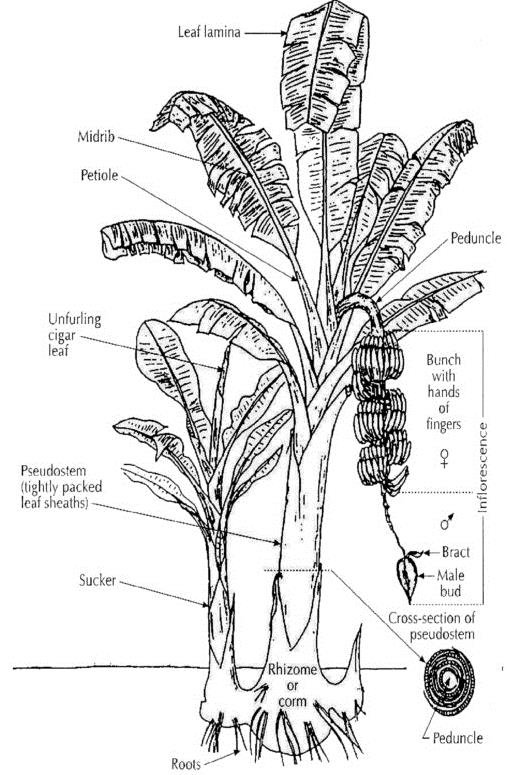
\includegraphics[width=12cm]{Figures/Diagrammatic-representation-of-a-fruiting-banana-plant-with-suckers-in-Bakry-et-al_W640.jpg}
    \caption[Anatomy of fruiting banana plant]{\textbf{Anatomy of fruiting banana plant} (From \textcite{Bakry2009}).}
    \label{fig:Anatomy of fruiting banana plant}
\end{figure}
\clearpage

\subsection{The History of Banana}

Originating from Southeast Asia, naturally occurring parthenocarpic – developing fruit without fertilisation – individuals of banana have been cultivated for about 10,000 years. Evidence of this can been seen in \textit{Musa banksii} phytoliths discovered in the Kuk swamp in Papua New Guinea \parencite{Denham2011}. Cultivated bananas were spread from Papua New Guinea, hybridising with subspecies of \textit{M. acuminata} and \textit{M. balbisiana} in the Philippines and northern New Guinea \parencite{Perrier2009}. Triploid cultivars were produced as a consequence and were dispersed throughout Southeast Asia, Northern Australia, East Africa, and South Asia by the Austronesian peoples, where, although primarily cultivated as a food crop, banana was also used in traditional medicine to treat ailments including dysentery, ulcers, leprosy, epilepsy, and insect bites \parencite{Kumar2012}. In these regions, banana has also been used as fodder; in domestic materials, such as plates, children’s toys, and dyes; in building for shelter, rafts, or rope; and has significant social and cultural value, involved in many traditional rituals and customs \parencite{Hapsari2017} .  

Banana cultivation continued to move into the Middle East and Northern Africa from the centre of domestication in Southeast Asia, which can be seen in references to banana in historic texts such as Ibn al-'Awwam's 12th-century agricultural work, \textit{Kit\=ab al-Fil\=a\d{h}a} (Arabic:\\ \<كتاب الفلاحة>, lit. \textit{Book of Agriculture}) \parencite{Clement1866}. Later, during expeditions in Southeast Asia and Africa in the mid-1500s, bananas were encountered by Europeans who transported plants to South America where colonists established banana plantations to supply the USA and Europe \parencite{Guzman-Rivas1960, Salas-Pascual2022}. This legacy continues today, with over 70\% of the EU’s banana supply coming from South American countries \parencite{EuropeanUnion2022}.  

\subsection{Cultivation and Value of Banana}
\label{sec:cultivation}

Global production now takes place year-round in tropical and subtropical regions where plants are commercially grown as a monoculture crop, although plants are also cultivated by smallholders and in subsistence production systems \parencite{Viljoen2020}. Commercially, fruits are harvested within about 9-12 months of planting (either\textit{ in vitro} propagated material or suckers) and are grown as a ratoon crop – the plant is cut back to the rhizome once the fruit has been harvested and left to regrow – for several years, by which time yields will have reduced and a new plantation must be generated. 

Today, banana is frequently reported as one of the world’s top agricultural commodities, the annual global production of bananas (including plantain) steadily increased from 98.4 million tonnes in 2000 to an estimated 155.2 million tonnes in 2018  and global exports increased from 15,540 tonnes in 2011 to 20,465 tonnes in 2021 \parencite{FAO2022}. Despite this, only around 15\% of bananas produced worldwide are traded in international markets. The remaining 85\% are consumed locally, highlighting the value of bananas as a subsistence crop, illustrated in developing countries where fruits can account for 25\% of daily calorie intake and act as a source of income \parencite{FAO2019}. The world’s largest banana growers are India and China which produced over 30 million tonnes and 11 million tonnes in 2021, respectively \parencite{BananaLink2023} (Figure ~\ref{fig:bananaProdMap}).  Currently, up to 40\% of all global banana production (domestic and export markets) is reliant on the Cavendish bananas \parencite{Warman2018}, a triploid, clonally propagated subgroup deriving from \textit{M. acuminata}.

\begin{figure}[h!]
    \centering
    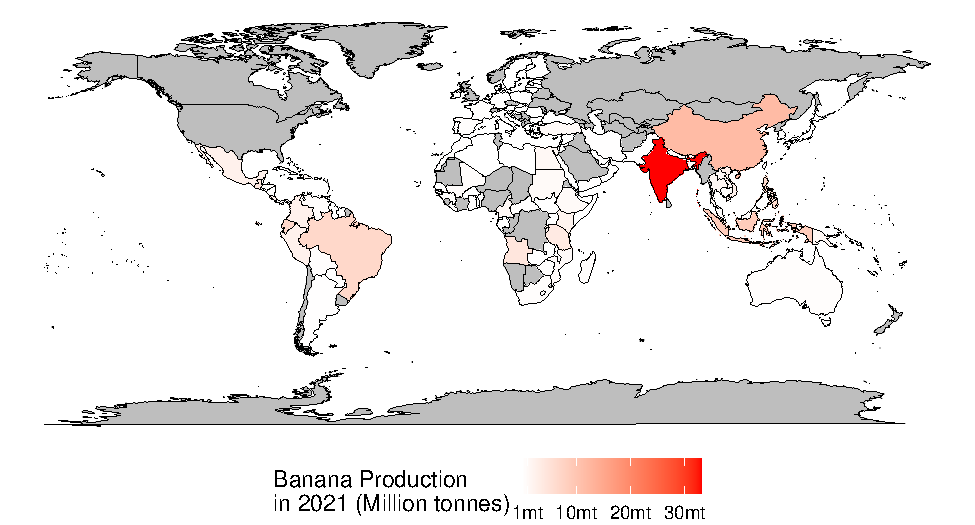
\includegraphics[width=\textwidth]{Figures/BananaProdMap.pdf}
    \caption[Global banana production, 2021]{\textbf{Global banana production (million tonnes), 2021.} No data available for countries in grey (Data source: BananaLink, 2023).}
    \label{fig:bananaProdMap}
\end{figure}

\section{Bananageddon: An Introduction to \acl{Focub}}
In recent decades, there have been reports of a potential ‘Bananageddon’, whereby global banana production is decimated by the fungal pathogen \acf{Focub} \acf{tr4}, the causative agent of \ac{fwb} (syn. Panama disease). The global banana community’s concern is demonstrated through the establishment of the \acs{tr4} Task Force, part of the \ac{FAO} \ac{wbf}; the Peruvian government’s declaration of a National Emergency upon the discovery of \ac{Focub4} in 2021 (FAO, 2021); and in the review by \textcite{Westerhoven2022}, where the authors stress \ac{Focub4}'s threat to African food security.   

\subsection{A Brief History of Fusarium Wilt}
\label{chap1:focHistory}
A robust response to \ac{Focub4} is not unfounded. During the first half of the 20th century, \ac{Focub1} \ac{r1} devastated global production, destroying  ~40,000 hectares of ‘Gros Michel’ plantations \parencite{Agrios2005, Kema2021}, and resulted in estimated economic losses of \$400 million (USD) between 1940 and 1960 (equivalently to \$4.117 billion or £3.259 billion)\parencite{Ploetz2005}. \ac{Focub1} eventually led to the disappearance of ‘Gros Michel’ as an export banana in the 1960s \parencite{Molina2007}, when the \ac{Focub1} resistant Cavendish bananas subsequently replaced ‘Gros Michel’ \parencite{Ordonez2015a}. 

The threat posed by \ac{Focub} remains, however. In the 1960s Cavendish banana plants in Taiwan were observed displaying symptoms of \ac{Focub} infection \parencite{Agrios2005}. Identified in 1994 as \acl{Focub4} \parencite{Ploetz1994} the strain affecting Cavendish bananas has continued to spread. \Ac{Focub4} is now found in Africa, Asia, and Europe \parencite{Ploetz2015a, Thangavelu2019} and is gaining a foothold in South America, with recent incursions in Columbia in 2019 \parencite{Garcia-Bastidas2019}, Peru in 2021 \parencite{Acuna2022}, and Venezuela in 2023 \parencite{Herrera2023}.

\subsection{Disease Development of \acl{Focub}}

As a soil-borne pathogen, \ac{Focub} first colonises the roots. Asexual spores in the soil germinate in response to host root exudates and infection hyphae produced from resting spores (chlamydospores) penetrate the root epidermis at the tip. \ac{Focub} hyphae progress through the root cortex to the rhizome and migrate through the xylem in the outer leaf sheaths of the pseudostem, occluding vessels and interfering with nutrient uptake and upward water transport; often before visible symptoms are observed \parencite{Li2017, Warman2018}. Two asexual spore types, microconidia and macroconidia, are produced within the xylem and help \ac{Focub} overcome some of the host’s barriers, such as naturally occurring end walls or perforation plates of the xylem strands, which somewhat restrict pathogen movement through the host \parencite{Dita2018}. Xylem vessels begin to collapse, and external symptoms are observed. Tissues become chlorotic and the plant withers as it transpires more than it can translocate. Once the plant dies, the fungus begins to invade other plant tissues and sporulate, particularly on the plant surface, producing chlamydospores (Figure: \ref{fig:MyLifeCycle}). Chlamydospores can persist in the soil for decades and are resistant to adverse conditions \parencite{Pegg2019}.  

Alternative hosts, including many grass and weed species, act as a reservoir of inoculum \parencite{Hennessy2005}.  \ac{Focub} is dispersed through the movement of contaminated plant and soil material, water, wind, and people. Typical symptoms of \ac{Focub} infection include discolouration and splitting of the pseudostem, yellowing of lower leaves often forming a ‘skirt’ around the plant, and a streaking pattern is occasionally observed on the foliage (Figure ~\ref{fig:FusariumWiltSymptoms}). 

\begin{figure}[p!]
    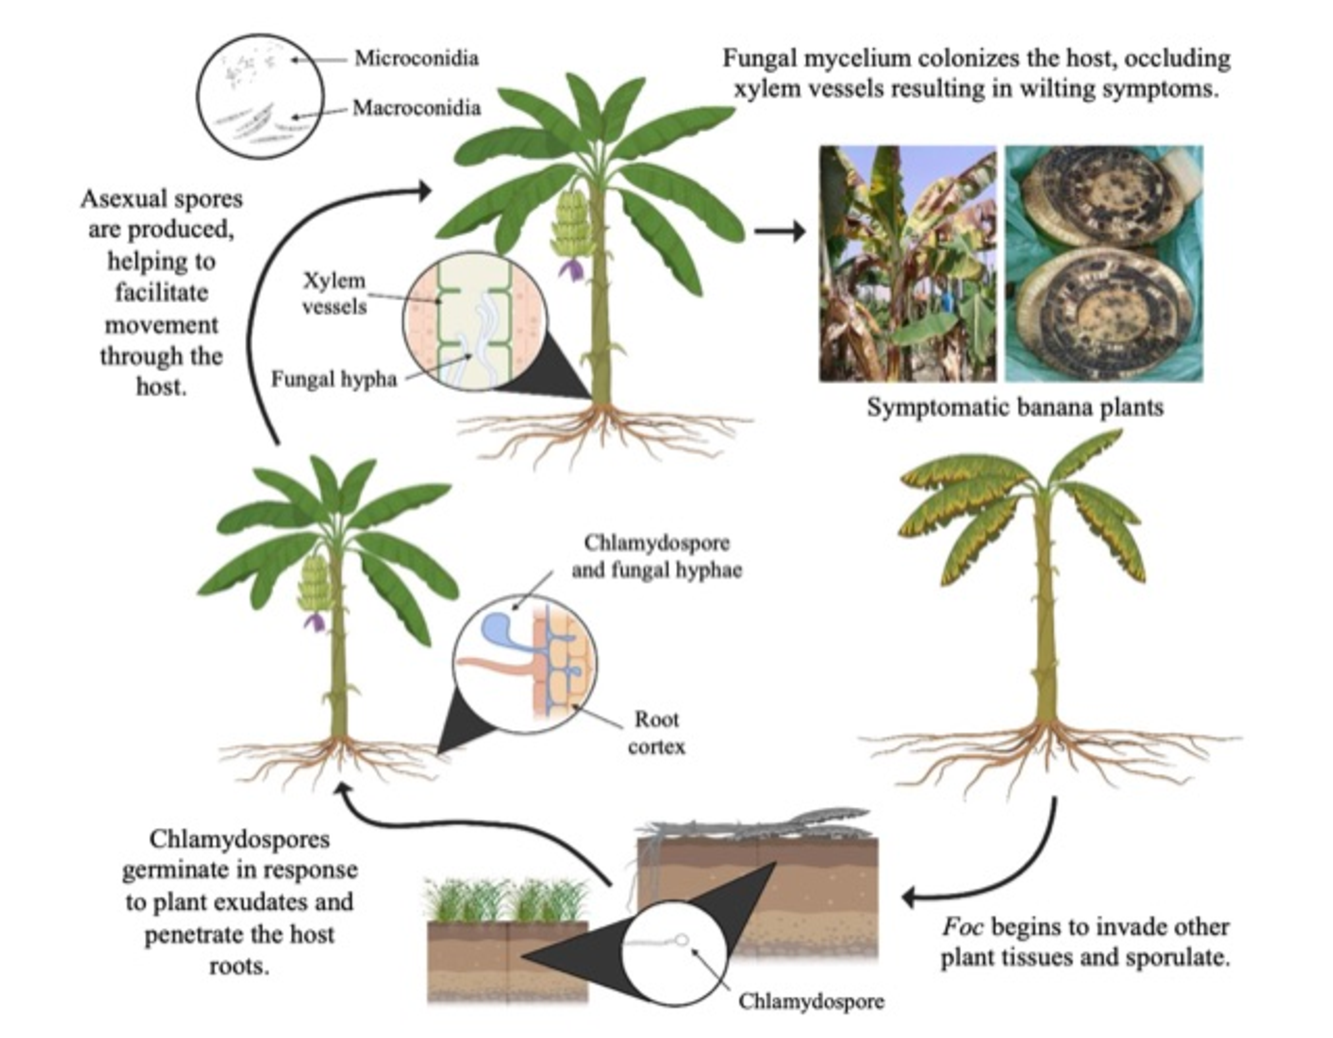
\includegraphics[width=16cm]{Figures/MyLifeCylceNarrow.pdf}
    \caption[Fusarium wilt of banana disease cycle.]{\textbf{Fusarium wilt of banana disease cycle.} Chlamydospores germinate in the soil in response to plant root exudates. Infection hyphae from chlamydospores penetrate the root tip epidermal cells and progress through the host root cortex to the xylem. Microconidia and macroconidia are produced in the xylem and help to facilitate pathogen movement through the host. As \acl{Focub} migrates through the xylem it occludes vessels and interferes with nutrient uptake and upward water transport. External wilting symptoms begin to develop; tissues become chlorotic and the plant withers as it transpires more than it can translocate. Eventually, the plant dies, and asexual spores are formed on the dead tissue. Chlamydospores persist in the soil or \acl{Focub}  survives endophytically in an alternative host species. Fungal hyphae are shown in blue. Images of \acl{Focub}  spores adapted from \textcite{Fourie2011} and symptomatic banana plant images sourced from \textcite{Maymon2020}. Figure created with BioRender.com.}
    \label{fig:MyLifeCycle}
\end{figure}

\begin{figure}[pt!]
    \centering
    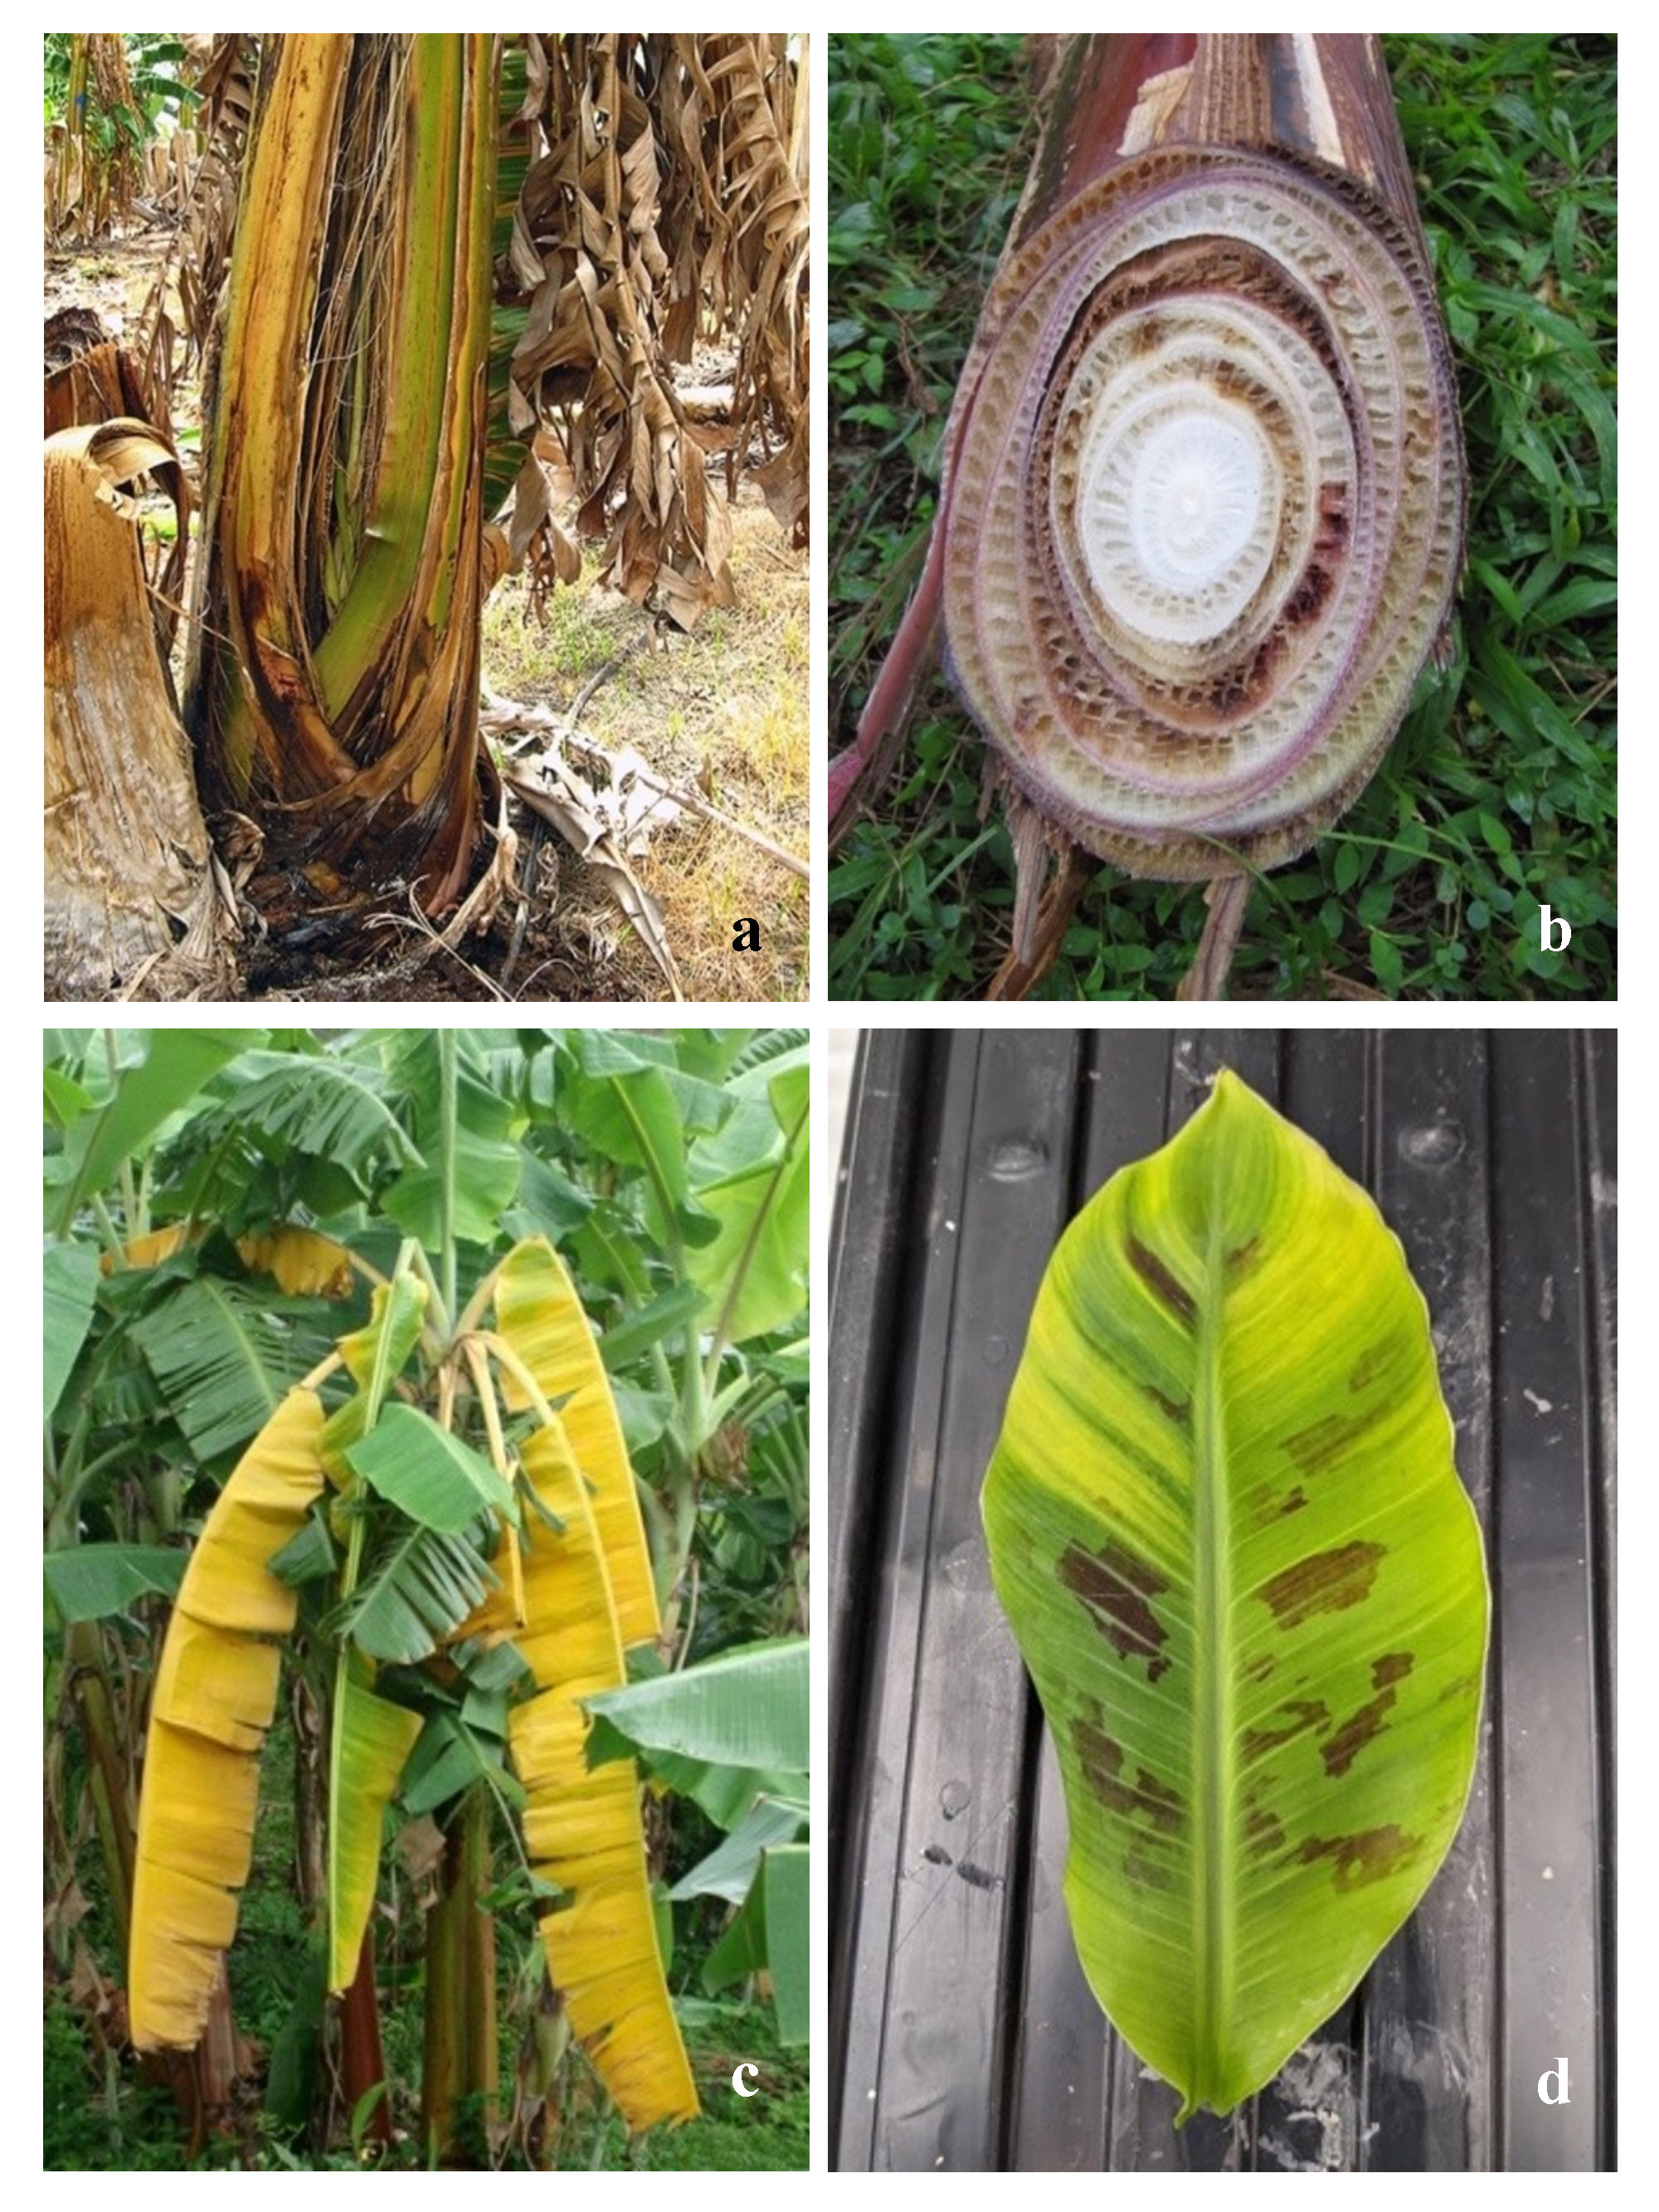
\includegraphics[width=15cm]{Figures/SymptomsofFoc.pdf}
    \caption[Typical symptoms of \textit{Fusarium}  wilt of banana.]{\textbf{Typical symptoms of \textit{Fusarium} wilt of banana.} (a) Splitting of the psuedostem, (b) discolouration of the psuedostem, (c) yellowing of lower leaves, and (d), a streaking pattern is observed on the foliage. Photos by Dita, M (a) and Blomme, G (b and c), Bioversity International.}
    \label{fig:FusariumWiltSymptoms}
\end{figure}

\subsection{Classification of \acl{Focub}}

\ac{Focub} belongs to the \ac{FOSC}. The species complex contains both plant and animal pathogens, as well as saprophytes and endophytes \parencite{Leslie2006}. \acs{Fo} has high functional and genetic diversity, shown plainly in its broad plant host range. The species complex can infect around 150 species of both monocotyledonous and dicotyledonous plants, including many horticulturally important crops such as banana, tomato, and lettuce \parencite{Edel-Hermann2019}.  Individual pathogenic \ac{Fo} isolates can infect only one or a few plant species. Plant pathogenic \ac{Fo} are therefore divided into ‘special forms’, or \acp{fsp}, each of which is adapted to specific hosts \parencite{Snyder1940}. For instance, strains which cause Fusarium wilt in tomato are classified as \acl{Foly}. To date, 106 \acp{fsp} have been clearly described and with at least an additional 37 putative \acp{fsp} \parencite{Edel-Hermann2019}.   

Some \acp{fsp} can be further subdivided into pathogenic races, determined by pathogenicity towards specific host cultivars. Three races of \ac{Focub} affecting banana have been identified. \acf{r1}  affects banana cultivars such as ‘Gros Michel’ (AAA), ‘Maqueno’, ‘Silk’, ‘Pome’ (AAB), and ‘Pisang Awak’ (ABB); \acf{r2} affects ‘Bluggoe’ and other cooking bananas (ABB); Race 4 affects the subgroup Cavendish (AAA) as well as hosts of \ac{r1} and \ac{r2} \parencite{Ploetz2015a} and has been further divided into \ac{str4} and \acl{tr4}. \Ac{tr4} is distinguished from \ac{str4} as it affects susceptible cultivars without disease-predisposing conditions \parencite{Ploetz2015b}.  

Classification of isolates based on race is often subjective. During the 1980s an additional method of \ac{Focub} identification based on \ac{vcg} was developed \parencite{Correll1991}. \acp{vcg} are comprised of isolates that possess the same alleles at all \ac{vic} loci, and so can form stable heterokaryons with each other \parencite{Correll1991}. So far, 24 \acp{vcg} of \ac{Focub} have been confirmed in \ac{Focub} (Table ~\ref{tab:VCGTab}) \parencite{Czislowski2018}, though \textcite{Mostert2022} have since reported additional \ac{Focub} \acp{vcg}. Some \acp{vcg} of \ac{Focub} are taxonomically closer to other \acp{fsp} of \ac{Fo} than other \ac{Focub} \acp{vcg}. This, coupled with distinct genetic lineages identified through phylogenetic analysis, has resulted in the recognition of a polyphyletic – taxonomic group including members from different ancestral lineages – evolutionary history for \ac{Focub} \parencite{Koenig1997, Ploetz2007}. 

\textcite{Maryani2019} revised the taxonomy of \ac{Focub}, generating the Fusarium of Banana Species Complex and proposing several new species. However, \textcite{Torres2021} have suggested that the revision is premature and that the data do not fully support the revision. There continues to be active debate surrounding \ac{Focub} classification and a clear, robust, universally accepted taxonomy has not yet been established. Race, although somewhat informal, remains the most widely accepted method of \ac{Focub} classification – whereby isolates are identified based on virulence towards specific host cultivars.  

\afterpage{

%Insert the VCG table
% Please add the following required packages to your document preamble:
% \usepackage{longtable}
% Note: It may be necessary to compile the document several times to get a multi-page table to line up properly
\begingroup
\setlength{\tabcolsep}{28pt} % Default value: 6pt
\renewcommand{\arraystretch}{0.75}
\begin{longtable}[tc!]{ccc}
\caption[\acf{vcg} of \ac{Focub}]{{\textbf{\acf{vcg} of \ac{Focub}} and race (Czislowski \et 2018).} Cross-compatible VCGs can form VCG complexes.}
\label{tab:VCGTab}\\
\hline
\textbf{VCG} & \textbf{VCG   complex} & \textbf{Race}    \\ \hline
\endfirsthead
%
\multicolumn{3}{c}%
{{\bfseries Table \thetable\ continued from previous page}} \\
\endhead
%
0120  & 0120–01215           & STR4             \\
0121  &                      & R4               \\
0122  &                      & R4               \\
0123  &                      & R1               \\
0124  & 0124–0125–0128–01220 & R1,   R2         \\
0125  & 0124–0125–0128–01220 & R1, R2           \\
0126  &                      & R1               \\
0127  & No longer valid      & No longer valid  \\
0128  & 0124–0125–0128–01220 & R1,   R2         \\
0129  & 0129–01211           & STR4             \\
01210 &                      & R1               \\
01211 & 0129–01211           & STR4             \\
01212 &                      & Not   Identified \\
01213 & 01213–01216          & TR4              \\
01214 &                      & R2               \\
01215 & 0120–01215           & STR4             \\
01216 & 01213–01216          & TR4              \\
01217 &                      & R1               \\
01218 &                      & R1               \\
01219 &                      & Not identified   \\
01220 & 0124–0125–0128–01220 & R1               \\
01221 &                      & Not Identified   \\
01222 &                      & Not   Identified \\
01223 &                      & Not Identified   \\
01224 &                      & Not   Identified \\ \hline
\end{longtable}
\endgroup

\clearpage
}

\subsection{The \acl{Fo} genome} 

An emerging explanation for shared host specificity between different \acf{Fo} lineages relates to the compartmentalisation of the \ac{Fo} genome, a theory that has become increasingly prevalent in \ac{Fo} genomics following the work of \textcite{Ma2010}. This study explains that the \textit{Fusarium} genome can be organised into two parts containing either \acp{cc} or \acp{ac} (syn. pathogenicity/lineage-specific/supern\-umerary chromosomes). The 11 \acp{cc} within the \ac{Fo} genome encode functions necessary for primary metabolism and reproduction \parencite{Dam2017}. The remaining \acp{ac}, which vary in number among \acp{fsp}, are not required for primary metabolism and reproduction, contain secondary metabolite biosynthetic gene clusters, encode virulence genes such as effectors, and possess a high number of \acp{te} \parencite{Ma2010, Schmidt2013, Witte2021}. Further, \textcite{Ma2010} suggests these \acp{ac} can be horizontally transferred and afford host-specific pathogenicity to the recipient. A theory which has since been demonstrated in \ac{Foly} \parencite{Vlaardingerbroek2016a, Vlaardingerbroek2016b, Li2020a}, \ac{Fo} f. sp. \textit{radicis-cucumerinum} \parencite{Dam2017} and \ac{Fo} f. sp.  \textit{melonis} \parencite{Li2020b}. 
 
Not only do \acp{ac} go some way to explaining diversity between \acp{fsp}, but also among strains within specific \ac{fsp}. For instance, a recent preprint by \textcite{Westerhoven2023} analyses the dynamics of \acp{ac} in \ac{Focub} and explores the role segmental duplications have in \ac{ac} evolution and diversity within \ac{Focub}. \textcite{Westerhoven2023} sequenced and assembled 69 \ac{Focub} strains (including \ac{r1}, \ac{r2}, and \ac{tr4})  isolated from various banana-growing regions. They generated chromosome-level genome assemblies and identified \acp{ac} in these strains.  The authors reported a significant amount of variability of the \acp{ac} between the \ac{fwb} strains, for instance, \acp{ac} ranged in size from 6.7Mb to 16.5Mb and exhibited extensive diversity in gene content, repeat content, and GC content when compared to the \ac{Focub} core chromosomes. \Acp{ac} are most commonly shared among strains of \ac{Focub1} from the same lineages, and few \acp{ac} are shared between \ac{r1} lineages. \Acp{ac} in \ac{Focub4} strains, however, showed low nucleotide diversity and the authors suggest that \ac{Focub4} evolved from a single recent clonal origin. 

The manuscript by \textcite{Westerhoven2023} highlights the prevalence of segmental duplication in \acp{ac} and sub-telomeric regions of \ac{Focub}. The authors demonstrate that these duplications are associated with the recent evolution and diversification of genes, including virulence genes, and play a crucial role in the expansion and adaptation of \acp{ac} in the \ac{FOSC} genome. However, it is worth noting that this manuscript has not currently published the \ac{Focub} assemblies generated, nor does it provide an appropriate data set detailing the assembly quality of the isolates sequenced for the study, making it challenging to validate the authors' conclusions. 

\subsection{The Plant Innate Immune System}

As a plant pathogen, \ac{Fo} faces considerable evolutionary pressure to develop diverse mechanisms that can evade host detection and facilitate successful infection. Due to the relatively recent evolutionary history of \acp{ac}, wide diversity, ability to function separately from \ac{Fo}'s \ac{cc}, and a high number of \acp{te} suggests that this specific section of the genome serves to fulfil the pathogen's adaptive needs in its interaction with hosts and evade plant defence mechanisms.

Plants have coordinated defence mechanisms which enable them to detect and respond to invading pathogens effectively. The plant’s innate immune system is comprised of two interconnected tiers which perceive and respond to pathogen infection \parencite{Jones2006, Han2019, DeFalco2021}. The first tier recognises microbial- or \ac{pamp} which are slow-evolving, conserved molecules (such as the fungal cell wall component, chitin) using transmembrane \ac{prr} on the plant cell surface. Once \ac{pamp} have been recognised, \ac{pti} is induced, including numerous cell signalling events such as altered ion fluxes, the production of apoplastic reactive oxygen species, callose deposition, and transcriptional reprogramming. 

To evade, suppress or interfere with \ac{pti} responses and establish infection, fungal pathogens secrete proteins termed ‘effectors’ into the host cell which results in \ac{ets}. To combat \ac{ets}, plants possess a suite of \ac{rprot} which perceive effectors (termed '\ac{AVR} proteins') and induce further immune responses, known collectively as \ac{eti} \parencite{Jones2006} (Figure:~\ref{fig:PlantImmuneSystem}). \Ac{rprot} are conserved intracellular receptors of the \ac{nlr} class. The structure, function, and effector perception (direct or indirect) of \ac{rprot} is variable and often specific (see: \textcite{Chen2022, Wang2022}). Similarly, effectors are typically highly variable and specific to individual pathogens \parencite{LoPresti2015}. \textcite{Gutierrez2023} have prepared a comprehensive review of virulence factors in the \textit{Fusarium} genus. 

\begin{figure}[h!]
    \centering
    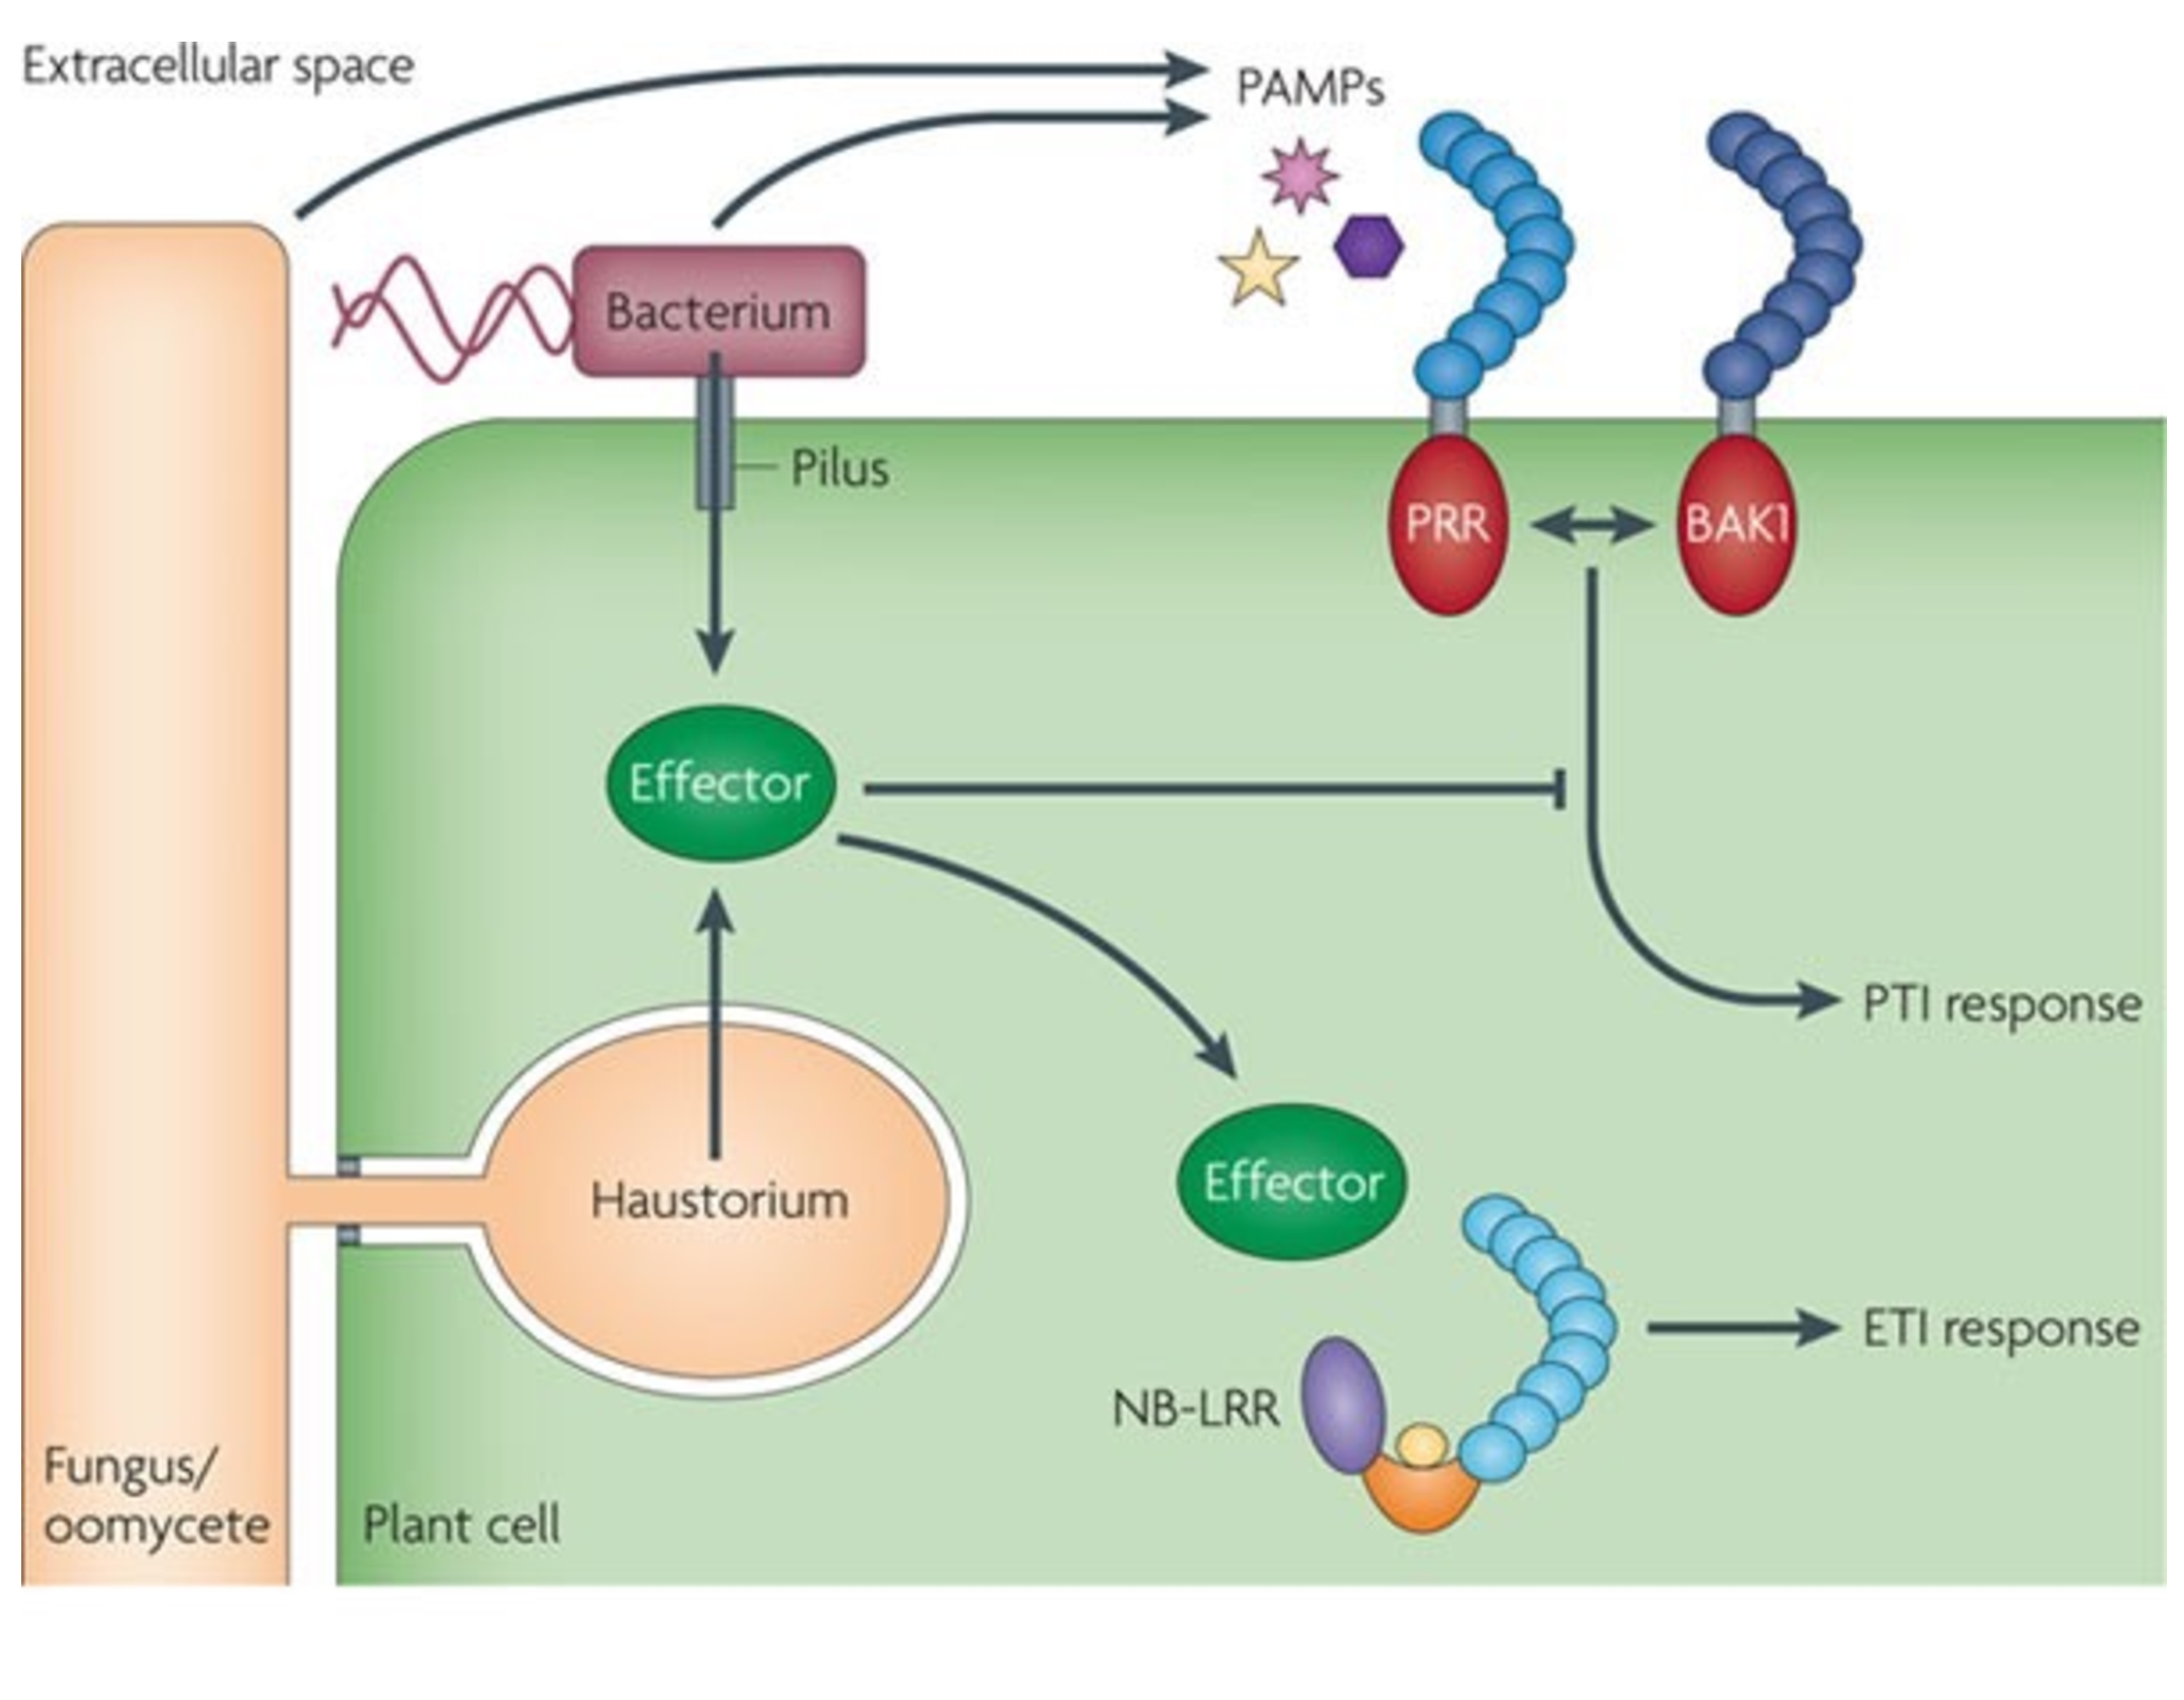
\includegraphics[width=\textwidth]{Figures/DoddsArticleModel.pdf}
    \caption[Overview of the plant immune system.]{\textbf{Overview of the plant immune system.} Pattern recognition receptors (PRRs) perceive microbial- pathogen-associated molecular patterns (MAMPs/PAMPs) and induce a PAMP-triggered immunity (PTI) response from the host. To overcome host cell defences, pathogens secrete small molecules known as effectors into the host cell, inducing effector-triggered susceptibility (ETS). Plants have adapted a family of resistance proteins (R proteins), which can perceive pathogen effectors (avirulence proteins) and stimulate an effector-triggered immunity (ETI) response from the plant host (From Dodds and Rathjen, 2010).}
    \label{fig:PlantImmuneSystem}
\end{figure}


\subsection{The \acl{Fo} Effectorome}
\label{Chap1:fusariumEffectorome}

In the \ac{FOSC}, the only family of effectors currently recognised are the \acp{sixg}. In total, 14 SIX proteins (SIX1 – SIX14) have been identified through mass spectrometry of infected tomato xylem sap and whole genome sequencing \parencite{Houterman2007}.  All 14 \acp{sixg} are found on the \acp{ac} in \ac{Foly} \parencite{Schmidt2013}, and studies have confirmed that \textit{SIX1, SIX2, SIX3, SIX5}, and \textit{SIX6} are essential for conferring virulence in tomato, with  \textit{SIX4} (\textit{Avr1}), \textit{SIX3} (\textit{Avr2}), and \textit{SIX1} (\textit{Avr3}) all recognised by corresponding \ac{rprot} (called ‘I-’ for Immunity) in tomato \parencite{Rep2004, Lievens2009, Takken2010, Gawehns2014, Ma2015}. Since their discovery in \ac{Foly}, homologs of \acp{sixg} have been identified in other \acp{fsp}, including \textit{cepae, conglutinans, fragariae, melonis, pisi, radicis-cucumerinum,} and \textit{vasinfectum} \parencite{Czislowski2018}. A further \textit{SIX} gene, (\textit{SIX15}) has been described by \textcite{Simbaqueba2018} in \acl{Fo} f. sp. \textit{physalis}, although \textit{SIX15} is not widely reported. 

In \ac{Focub}, homologs of \textit{SIX1, SIX2, SIX4, SIX6, SIX7, SIX8, SIX9}, and \textit{SIX13} have been identified, and \textit{SIX1} and \textit{SIX8} have been recognised in \ac{Focub} \ac{tr4} as essential for virulence through knockout mutants \parencite{Widinugraheni2018, An2019}. Interestingly, \textcite{Fraser-smith2014} observed differences in \textit{SIX8} sequence between \ac{r4}, \ac{str4}. \textcite{Czislowski2018} reported differences in the \ac{sixg} repertoire of \ac{Focub} \ac{r1} and \ac{r4} lineages and hypothesised that the differences in \ac{sixg} profiles contribute to the variability in the \ac{Focub} host cultivar range.  However, as suggested, \acp{sixg} are unlikely to be the only set of effectors involved in host specificity, and state "it should be expected that novel and undiscovered effectors remain to be identified in the lineages of \ac{Focub}" \parencite{Czislowski2018}.  

\textcite{Ma2010} showed that the \acp{ac} in \ac{Foly}, have a high number of retro-elements, including the non-autonomous class II \acf{te}, \ac{mites}. A specific family of \ac{mites}, known as \acfp{mimp}, are found upstream of all known \acp{sixg} in \ac{Foly} \parencite{Schmidt2013}. Characterised by their \ac{tir} sequence and short length (180–220 \acs{bp}), \textcite{Schmidt2013} surmised that \acp{mimp} could be used for the prediction of effectors in \ac{Fo}, particularly \acp{sixg}, a theory later demonstrated by \textcite{Dam2016, Dam2017, Armitage2018, FoEC2}.  

The hypothesis that effector profiles contribute to host specificity is proposed for other \ac{fsp} \parencite{Achari2021, Batson2021} and is tested on the host species level for the \ac{FOSC} \parencite{Dam2016}. With advances in genome sequencing and analysis, it is possible to identify new candidate effectors using common characteristics shared between known effectors in \ac{Foly} and other \ac{fsp}, as well as their location in the \ac{Fo} genome and evolutionary relationship.

\subsection{Control of \acl{Focub}}

There are few effective controls for \ac{Focub} in the wider environment. Chlamydospores can persist in the soil for decades and \ac{Focub} can invade non-host plants and survive as an endophyte, with grass and weed species acting as sources of inoculum \parencite{Pegg2019}. Biological control agents and fungicides have been investigated as a means of \ac{Focub} control. However, most of these are \textit{in vitro} and greenhouse assays which, although successful, are not practical or effective in-field \parencite{Dita2018}.  

As most commercial bananas are triploid and parthenocarpic, conventional breeding for resistance is exceedingly challenging \parencite{Dale2017}. One somaclonal variant of Cavendish, ‘Formosana’ is marketed as being resistant to \ac{tr4}, however, yields are slightly reduced due to its longer growth cycle and there have been reports of  ‘Formosana’ showing \ac{tr4} susceptibility in later field trials \parencite{Lee2011, Dale2017}. A further somaclonal variant, ‘Guijiao 9’, is also marketed as showing lower disease severity compared to conventional commercial Cavendish varieties such as ‘Williams’ \parencite{Sun2019}, but the variety has only recently been released to the market and field trials outside of the region, in which this variety was developed, have not yet been conducted.  

Advances in genetic modification technologies have facilitated the development of two \ac{tr4}-resistant transgenic Cavendish lines \parencite{Dale2017}. One of these lines, ‘QCAV-4’ is currently undergoing regulatory approval in Australia \parencite{Lu2023}. The transgenic 'QCAV-4' variety was generated by transforming \textit{M. acuminata }Cavendish cv. 'Grand Naine' (AAA subgroup) embryogenic cell suspensions (prepared from immature male flowers) using the centrifugation assisted \textit{Agrobacterium tumefaciens}-mediated method with \ac{rga2}. \ac{rga2} is a putative \ac{nlr}-type \ac{rgene} from a seedling of \textit{M. acuminata} ssp. \textit{malaccensis} with resistance to \ac{Focub4}. However, the market for genetically modified crops within Europe is limited, although debate and legislation are currently under review and development. 

Gene-edited banana may be a more marketable alternative, particularly for Europe, and editing for disease resistance has been demonstrated in banana. \textcite{Tripathi2021} used CRISPR-Cas9 to make mutations to the downy mildew resistance 6 (DMR6) orthologue in banana, showing enhanced resistance to the bacterial pathogen \ac{xvm}, this approach may be applied to target a gene which could provide resistance to \ac{Focub}.  

\section{Bananomics: Tools and Technologies to Identify \textit{Fusarium} Wilt of Bananna}
\label{sec:chap1-diagnostics}

Prevention of \ac{Focub} introduction has so far proven the most effective method of \ac{Focub} control on a large scale \parencite{Ploetz2015b}, with management primarily focused on hygiene practices and prevention. The development of accessible, fast, and accurate diagnostic tools is imperative. Molecular and image-based diagnostics have both been developed to identify \ac{Focub}. However, many of the current image-based diagnostics are unable to distinguish \ac{Focub} from other banana wilt pathogens, and the molecular assays struggle to accurately identify pathogenic races.  

\subsection{Molecular Diagnostic Approaches}
\Ac{pcr}-based methods of identification are routinely employed in the detection of \ac{Focub}, alongside \ac{vcg} screening and race typing. Assays have been developed by \textcite{Lin2009, Dita2010, Li2013a, Li2013b}. A study by \textcite{Magdama2019} reviewed the efficacy of these \ac{pcr}-based detection methods for the identification of \ac{Focub4} against 302 \textit{Fusarium} isolates, including 292 \ac{Fo} isolates. The authors demonstrated that the primers developed by \textcite{Lin2009, Li2013a} for \ac{str4} and \ac{tr4} identification displayed false positives for \ac{r1} and \ac{r2} as well as five non-pathogenic \ac{Fo} endophytes. Similarly, primers developed by \textcite{Dita2010} showed false positives for \ac{Fo} endophytes. 

\textcite{Magdama2019} concluded that the most effective primers for \ac{tr4} identification are those developed by \textcite {Li2013b} and that, due to the diversity of the \ac{FOSC}, a wider range of \ac{Fo} isolates should be assessed when developing assays, and that primer design should focus on a genetic locus related to virulence to limit false positives.  Indeed, the gene targeted for diagnostics by \textcite {Li2013b} was implicated in virulence as a result of a T-DNA insertion conferring reduced virulence. However, to date there has been  no further characterisation of the gene by deletion, editing, or complementation to confirm its function.  

\textcite{Ordonez2019} used genome data and Diversity Array Technology sequencing to identify new genomic markers for \ac{Focub4} identification and develop a \ac{lamp} assay for in-field \ac{Focub4} diagnostics. The \ac{lamp} primers were assessed for specificity against 67 isolates, including 22 \ac{tr4} isolates, 28 alternative \ac{Focub} \acp{vcg}, 16 other \ac{Fo} \ac{fsp} isolates, and one \textit{Ralstonia solanacearum} isolate. Although thorough, \textcite{Ordonez2019}  did not survey as many isolates as \textcite{Magdama2019}. Further research is required to determine if the sequences identified adhere to the recommendations of \textcite{Magdama2019}. 

\subsubsection{Effectors as a Target for \acl{Focub} Diagnostics}

Ideally, to develop molecular diagnostics that successfully distinguish between various \ac{Focub} races, \ac{Fo} \ac{fsp}, and endophytes, a key genetic locus with an important role in pathogen virulence, such as effectors, should be targeted. Since the review by \textcite{Magdama2019}, diagnostic assays using \ac{pcr}-based methods targeting \ac{sixg} in \ac{Focub} have been developed by \textcite{Carvalhais2019}. These assays include simplex and duplex \acp{pcr} with additional restriction digestion steps. Primers specifically amplify regions of \textit{SIX6} in \ac{r1}, \textit{SIX1} in \ac{tr4}, \textit{SIX8} in \ac{str4}, \textit{SIX9/SIX10} in \ac{Focub} \ac{vcg} 0121 (R4), and \textit{SIX13} in \ac{Focub} \ac{vcg} 0122 (R4). The assays were validated using 250 \textit{Fusarium} isolates, including 16 different plant-associated \textit{Fusarium} species and 21 \acp{vcg}  commonly associated with \ac{Focub}. Amplicons were not generated for 5 of the 65 \ac{r1} isolates and the assay for \ac{Focub} \ac{vcg} 0121 generated false positives for three out of the 32 \ac{tr4} isolates. Furthermore, no known \ac{r2} isolates were used when validating the assays. Although effective in identifying isolates within R4, these assays arguably lack specificity for effective, accurate diagnostics of \ac{r1}, and specific groups within R4, and may provide false positives should an \ac{r2} isolate be sampled. This study indicates that \acp{sixg} provide a potential target for \ac{Focub} diagnostics, and access to a greater number of \ac{Focub} genomes may allow for more accurate primer development.  

\textcite{Chang2020} identified putative effectors in \ac{Focub} using a \ac{mimp}-based approach. They identified candidate effectors in \ac{Focub} by searching local genome databases of \ac{Focub1} and \textit{Foc} R4 using 13 \ac{mimp} sequences from \textcite{Dam2016}. They identified 20 candidate effectors; 3 unique to \ac{Focub1}, 6 unique to \textit{Foc} R4. To demonstrate the accuracy of their identification method, they generated a knockout mutant and its complement of one candidate effector, gene \textit{Foc 1324}. Virulence tests on banana plants demonstrated that \textit{Foc 1324} was a virulence factor required for the pathogenicity of \textit{Foc} R4. Confirmation of function is still required for all candidate effectors in this study. Furthermore, candidate effectors were only identified in two genomes, one \ac{r1} genome and one R4 genome, \acp{vcg} for these genomes are not provided. Candidate effectors which \textcite{Chang2020} report are unique to \ac{r1} and R4 require further validation using more genomes representing different \ac{Focub} races.

Interestingly, the 13 mimp sequences identified by \textcite{Dam2016} in \ac{Focub} were found across three isolates, a considerably lower number of \acp{mimp} compared to other \acp{fsp} in their study. Our investigations revealed that the method of \ac{mimp} identification employed by \textcite{Dam2016} was flawed, being case sensitive (only searched for capitalised \ac{mimp} \acp{tir})\footnote{We made the authors aware, and they have subsequently updated their tool. See \textcite{FoEC2} }. Two of the \ac{Focub} genomes (B2 and N2) used had been repeat masked, therefore many potential \acp{mimp} in \ac{Focub} are likely to have been missed. A greater number of \ac{mimp}-associated effectors could have been discovered by \textcite{Chang2020} should they have had a query set of \ac{mimp} sequences more representative of those in \ac{Focub}.

%\subsection{Image-based Approaches for Disease Diagnosis in Banana}
 
 %Non-invasive technologies, such as \ac{rs}, can help to monitor plant pathogens and, employed alongside molecular diagnostics, can be used for disease diagnosis \parencite{West2010}. As \ac{rs} technologies have advanced and increased in popularity, a wealth of multispectral, hyperspectral, thermal, RGB, and radar imaging data have been generated. These data have been employed in mapping and quantifying pathogens, providing a perspective on pathogen movement at multiple scales, helped to generate epidemiological models, and control disease spread \parencite{Zhang2019}.

%Satellites, such as Landsat and Sentinel, which make data freely accessible, combined with aircraft, \acp{uav}, and tractors fitted with \ac{rs} technologies, have collectively and increasingly been employed in plant disease management. Satellites have become popular for mapping disease spread at a large spatial scale. Accurate detection of disease from satellites requires not only a high enough resolution, but also favourable weather conditions and can be influenced by the satellite revisit period \parencite{Zhang2020}. Other technologies, such as \acp{uav} and tractors, have enabled field and sub-field scale detection of diseases in a variety of crops, and have become a key component of precision agriculture. Again, these technologies are affected by resolution and weather conditions, however, unlike satellites, the timing of application and distances from the crop (affecting resolution) can be easily manipulated.  

%\Ac{rs} technologies are used to observe changes in the optical properties of leaves or crop canopies. Disease symptoms are typically identified in the visible (VIS = 400\textendash700nm), near-infrared (NIR = 700\textendash1,200nm), and shortwave infrared (SWIR = 1,200\textendash2,400nm) spectral bands, using either passive sensors (i.e. sensors measuring the reflectance of solar radiation) or active sensors (i.e. systems equipped with an own source of radiation which their sensors record) \parencite{Mahlein2016}.  

%In healthy plants, due to the absorption of blue, yellow, and red bands by photoactive pigments (e.g. anthocyanins, carotenoids, chlorophylls), leaves typically exhibit low reflectance as VIS wavelengths. Similarly, water and leaf chemical components (e.g. proteins, lignin, cellulose) absorb SWIR resulting in low reflectance at the SWIR range \parencite{West2010}. Conversely, healthy plants exhibit high reflectance at the NIR range, as cell arrangement in leaf mesophyll tissue causes multiple scattering of NIR spectral bands \parencite{Ollinger2011}. In diseased plants, divergence from these optical properties can be observed. As a consequence of photochemical pigment degradation/destruction, necrotic or chlorotic lesions on appear on leaves, which, alongside pathogen propagules, cause increased reflectance in the VIS range. Similarly, increased reflectance in the SWIR range can be observed where pathogenesis affects water content, senescence and reduced growth, while defoliation drives decreased reflectance in the NIR range.   

%Many \ac{rs} studies have been conducted for the diagnosis of disease in banana, including those by \textcite{Johansen2014, Liao2018, Ochoa2016, Calou2020}. With additional studies by \textcite{Ye2020a, Ye2020b, Selvaraj2019, Zhang2022} focusing specifically on \ac{Focub}. All studies mentioned managed to successfully diagnose \ac{fwb}, distinguishing healthy plants from those infected with \ac{Focub}. Spectral reflectance proves effective in diagnosing \ac{fwb}, yet understanding the underlying biological mechanisms behind the observed spectral differences and distinguishing them from other stresses such as drought and vascular wilt pathogens like \ac{xvm} remains a challenge.

%\textcite{Marin2020} assessed the efficacy of \ac{rs} to distinguish water-stressed tomato plants from those infected with \ac{Fo} Fo5 strain isolated from \textit{Passiflora edulis} (passionfruit). The study showed that diseased plants could be distinguished from those subjected to hydric stress at 448–523nm, 624–696nm, 740–960nm, 973–976nm, and 992–995nm. However, these results were derived from multivariant analysis, whereby reflectance was correlated with the net assimilation rate of CO\textsubscript{2}, intercellular CO\textsubscript{2} concentration, stomatal conductance, transpiration rate, quantitative yield of \ac{ps2}, and continuous fluorescence. There is little indication that a single method of physiological stress measurement and its relationship to reflectance could be used to distinguish water stress from disease symptoms. One has to question how viable such multivariant analysis is as a means of diagnosis in the field. Is it practical or cost-efficient to measure these photosynthetic parameters in-field and correlate this with spectral reflectance to determine if plants are infected, or would alternative diagnostics be more effective and efficient?   

\subsection{Exploring Disease Biomarkers: Untargeted Metabolomics in Plant Systems}
\label{section:BiomakerIntro}

Though a robust response to \ac{Focub4} is essential to avoid a recurrence of the situation caused by \ac{Focub} in the early 20\textsuperscript{th} century (see: \ref{chap1:focHistory}), \ac{Focub} is not the sole threat to current banana production. \textcite{Ploetz2015c, Bebber2023} outline major current threats to banana production, including several biotic and abiotic wilting stresses: \acf{fwb} caused by \ac{Focub}, \acf{xwb} caused by \acf{xvm}, Moko/Bugtok disease caused by \textit{Ralstonia solanacearum}, banana blood disease caused by \textit{R. syzygii} subsp. \textit{celebesensis}, and climate change, particularly changing temperatures, rainfall, and access to irrigation. Additionally, the range of plant pests and pathogens is predicted to expand as a result of climate change \parencite{Bebber2015}, potentially exposing bananas to novel pathogens.

Growers must be able to accurately distinguish these various threats to ensure the correct treatment. It has been frequently reported that the symptoms of \ac{Focub} and \ac{xvm} can be challenging to distinguish for banana growers \parencite{Stellenbosch24, PromusaSymps, Biruma2007}, particularly foliar symptoms. In \ac{Focub}-infected plants, foliar chlorosis and wilting progress from older to younger leaves, often causing detachment at the petiole. Conversely, in \ac{xvm}-infected plants, symptoms of wilt can start from any leaf, with leaves sometimes later snapping along the blade. 

While \ac{pcr} assays offer a means to identify specific pathogens like \ac{Focub}, distinguishing between biotic stressors such as \ac{Focub} or \ac{xvm}, and abiotic stressors like drought, can be challenging. For instance, a negative \ac{pcr} result for \ac{Focub} does not necessarily imply the presence of drought stress. Additional \ac{pcr} tests can be used, but this comes with common challenges, including increased time, costs, and expertise required.

An alternative avenue for exploration is the application of metabolomics to identify novel diagnostic targets capable of accurately distinguishing between these biotic and abiotic stresses. Metabolomics, the analysis of a spectrum of metabolites in a biological system \parencite{Klassen2017}, while not fully harnessed for banana stress diagnostics, presents a promising direction for future research. Uncovering biomarkers indicative of specific stressors could revolutionise our ability to pinpoint the cause of wilting in banana plants.

Increasingly used in biomarker discovery \parencite{Li2016, Dang2018, Chen2023}, metabolomics, falls into two categories: targeted and untargeted analyses. Targeted metabolomics (TM) focuses on a specific set of compounds for precise quantitative analysis, often requiring intricate extraction protocols. \acf{um} seeks to identify a wide range of features without predefined targets, allowing the discovery of diverse, previously unknown compounds and metabolites. While \ac{um} employs simpler extraction and detection procedures compared to targeted studies, it generates highly complex datasets and comes with an increased challenge of false discoveries. As a result, \ac{um} demands substantial effort in data analysis and interpretation.

\ac{um} has been applied in the development of human disease diagnostics, providing insights into disease progression and revealing novel metabolites associated with diseases. \textcite{Masarone2021} used \ac{um} to analyse the metabolomic profiles of patients with \ac{nafld}, a condition including at least two different clinical entities, \ac{nafl} and \ac{nash}. \ac{nafl} has no (or rare) progression, whereas \ac{nash} causes liver cirrhosis, Hepatocellular Carcinoma, and liver-related deaths. The authors state that it is often challenging for hepatologists to distinguish between \ac{nafl} and \ac{nash} and go on to use \ac{um} to identify different biomarkers of \ac{nafld} to distinguish \ac{nafl} and \ac{nash}. \textcite{Masarone2021} demonstrate a significant separation between \ac{nafl}, \ac{nash}, and \ac{nash}-cirrhosis patients using a PLS-DA analysis. Some metabolites, marked by the authors "VIP", served as effective differentiators based on the severity of liver disease. These "VIP" metabolites included amino acids, glutathione, xanthine, and fatty acids. The authors suggest that these "VIP" metabolites can potentially be used for diagnosing and assessing \ac{nafld}.

\ac{um} has recently been used to identify biomarkers of susceptibility and resistance in plant pathology as well. For instance, \textcite{Sambles2017, Sidda2020} identified that some secoiridoid glycosides can be used as discriminatory metabolites of ash dieback  (caused by the fungus \textit{Hymenoscyphus fraxineus}) resistance and susceptibility,  in both UK and Danish ash trees (\textit{Fraxinus excelsior}). Studies in banana are limited, however. Most banana metabolomic studies pertain to the fruit and diet, with very few investigating the \textit{Foc}-banana metabolome. \textcite{Li2013c} assessed the virulence of \ac{Focub} isolates and used LC/MS/MS to determine the content of two mycotoxins consistently associated with \ac{Focub}, beauvericin and fusaric acid, in the roots, fruits, pseudostems, and foliage of plants. They showed that virulence correlated well with toxin deposition and went on to investigate the natural occurrence of these toxins in field-grown plants displaying symptoms of \ac{Focub} infection. They found that, although present, the natural occurrence was too low to be of concern to human and animal health.

As far as we are aware, no studies have employed \ac{um} to capture a global \ac{Focub}-banana metabolomic profile. Building on the work of \textcite{Sambles2017, Sidda2020}, we develop a \ac{um} protocol for biomarker discovery in banana. This provides insight into the biological processes influencing differences between the various biotic and abiotic stresses  and can be used to identify specific markers of each stress.

\newpage
\section{Project Aims and Objectives}

The overall aim of this research is to apply different omic tools for the detection of \acl{Focub} \ac{tr4} in banana and contribute towards the understanding of \acl{Focub} classification, identification, infection and banana responses. 

\begin{enumerate}
    \item Build tools which aid in the identification of targets for molecular diagnostics and contribute to our understanding of \ac{Focub}-banana interactions as well as the evolutionary history, diversity, and classification of \ac{Focub}. 
    \item Develop molecular diagnostics which can be used to identify specific races of \acl{Fo}. \footnote{Due to challenges sourcing isolates and sequence information from collaborators in Tamil Nadu Agricultural University, India (TNAU), our effector identification tool cannot currently be validated using \ac{Focub}. However, we are testing this tool using other \acl{Fo} \fancypagestyle{}{}{fsp} with collaborators at NIAB and the University of Warwick.} 
    \item Develop novel -omics approaches to improve understanding of banana interactions with \ac{Focub} and aid in the development of diagnostics.
\end{enumerate}

\newpage
\section{Thesis Structure}

\subsection{Chapter 2: A potential Novel Lineage of Banana Pathogens in \textit{Fusarium} Identified in India} 

This chapter reviews the genome assembly and subsequent analysis performed on \textit{Fusarium} isolates collected by collaborators at Tamil Nadu Agricultural University in India that are reported to be pathogenic on Cavendish banana. Phylogeny of isolates and geographic distribution are discussed and compared to publicly available genomes, and a potential novel species is presented. 

\subsection{Chapter 3: Improving Genomic Tools for Identifying Virulence Factors in \textit{Fusarium oxysporum}} 

This chapter describes our \acf{maei} tool which identifies putative effectors in \acl{Fo}, and the implications effector profiles have on the classification and genome compartmentalisation of the FOSC. \Acl{ce} presence/absence patterns, homology, and expression are explored. \Acp{ce} identified using the \ac{maei} tool may be used to identify targets of race-specific molecular diagnostics for \acl{Fo}.\footnote{This work is ongoing with collaborators at the University of Warwick, \ac{niab}, and Tozer seeds.} 

\subsection{Chapter 4: The Banana-pathogen Metabolome}

Banana disease imaging and \acl{um} analysis were conducted. This chapter
aims to help develop our understanding of the \acl{Focub} infection process and identify specific markers of infection from a variety of biotic and abiotic stresses. 

\subsection{Chapter 6: The Future of Fusarium Wilt of Banana Research is Multi-omic: A General Discussion}
This chapter discusses the main results from the thesis and draws overall conclusions. It also considers areas for improvement and future work. 


 

 



 



 



 
    
% \chapter{Potential Novel \textit{Fusarium} Pathogen of Banana Identified}
%     %%%%%%%%%%%%%%%%%%%%%%%%%%%%%%%%%%%%%%%%%%%%%
%INTRODUCTION
%%%%%%%%%%%%%%%%%%%%%%%%%%%%%%%%%%%%%%%%%%%%%
% Strcture
%----------
% - Pathogens spread 
% - Distribution of Foc is prime example 
% - TR4 is a strong reason to monitor the distribution and genetic makeup of Fwb pathogens.
% - Lack of data from world's largest producer and climate change is a threat. 
% - We're sequencing isolates...
%%%%%%%%%%%%%%%%%%%%%%%%%%%%%%%%%%%%%%%%%%%%%

\section{Introduction}
\label{sec:chap2Intro}

The history of \acf{Focub} exemplifies the profound impact pathogen spread and diversification can have on global crop production and economies. Although first reported in Australia in 1876 by \textcite{Bancroft1876}, current evidence suggests that the center of origin for \ac{Focub} is Southeast Asia, where it co-evolved with its \textit{Musa} host \parencite{Maryani2019}. Global banana cultivation inadvertently let to the introduction of \ac{Focub} to new regions, leading to severe damage to banana crops \parencite{Kema2021}. 

Notable early dispersion of \acs{Focub} \acf{r1} occurred in South America. The first reports in the region came from Panama and Costa Rica in the 1890s, where \ac{Focub1} acquired the common name, Panama disease \parencite{Ashby1913}. From there, \ac{Focub1}  spread across 'Gros Michel' plantations in Jamaica (1903), Suriname (1906), Trinidad and Tobago (1907), Cuba (1908), Guatemala (1910), Colombia (1929), and Venezuela (1930). By the mid-20th century, the banana export industry had been decimated by the \ac{fwb} epidemic. \Ac{Focub1} is now widely distributed in banana-producing countries, where it still affects many local varieties \parencite{Dita2018}.

Current global production of banana is dominated by the Cavendish variety, which takes its name from William Spencer Cavendish, the sixth Duke of Devonshire. Cavendish plants were originally brought to the duke's residence, Chatsworth House, Derbyshire, UK (1829) after their discovery in Southern China in 1826 by British colonial botanists. Shoots from Chatsworth's Cavendish were distributed to British colonies across the globe and resistance to \ac{Focub1} was eventually identified. By the 1950s the banana export industry had substituted the 'Gros Michel' variety for the Cavendish subgroup \parencite{Ploetz2005, Dita2018}. However, in the following decades, Cavendish banana plants in Taiwan displayed symptoms of \ac{Focub} infection \parencite{Agrios2005}. By the 1990s, the same strain of \ac{Focub} was devastating Cavendish plantations in Western Indonesia and the Malaysian peninsular \parencite{Kema2021}. 

Identified in 1994 as \ac{Focub} \acf{tr4} \parencite{Ploetz1994}, the race affecting Cavendish bananas has continued to spread. \Ac{Focub4} arrived in China from Taiwan in 1996, later expanding to Laos, Myanmar, and Vietnam. A first report was also recorded for Australia in 1997 \parencite{Ploetz2015a}. In 2005, \ac{Focub4} was recorded in the Philippines, rapidly spreading in Mindanao \parencite{Molina2009}. In the past 15 years, first reports of \ac{Focub4} have been published frequently, with occurrences in Pakistan (2012), Lebanon (2013), Oman (2013), Jordan (2013), Mozambique (2013), India (2015), Israel (2016), Colombia (2019), Peru (2021), and Venezuela (2023) (Figure \ref{fig:FocDis}) \parencite{Butler2013, Ploetz2015a, Ordonez2015b, Zheng2018, Thangavelu2019, Garcia-Bastida2020, Maymon2020, Kema2021, Acuna2022,  Herrera2023}.  The rapid expansion of \ac{Focub} poses a significant threat to global banana production, particularly in Asia, which serves as the centre of diversity for \ac{Focub}. Accurate monitoring of pathogen distribution and genetic diversity across the region is essential.  

\begin{figure}[h!]
  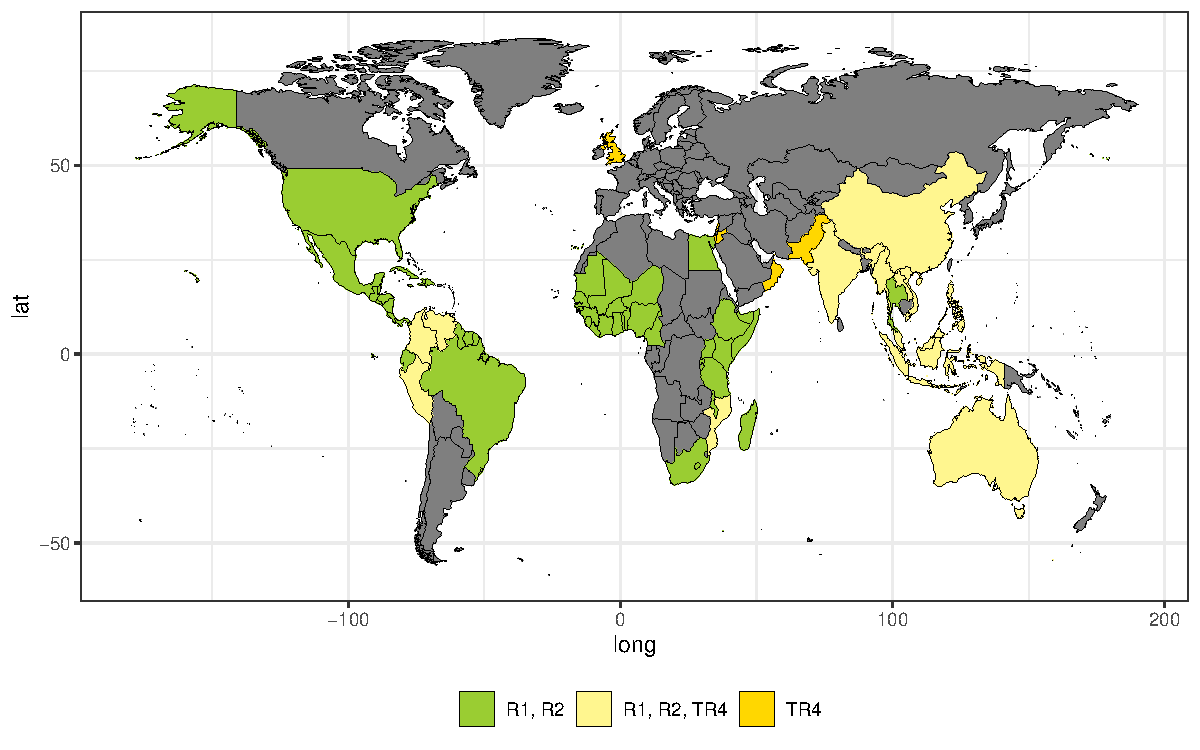
\includegraphics[width=14.5cm]{Figures/FocDis.pdf}
  \caption[Global Distribution of \textit{Fusarium oxysporum} f. sp. \textit{cubense}]{\textbf{Global Distribution of \textit{Fusarium oxysporum} f. sp. \textit{cubense}}. Presence or absence shown by country. Countries which have not reported \ac{Focub} are shown in grey. R1: Race 1, R2: Race 2, TR4: Tropical race 4.}
  \label{fig:FocDis}
\end{figure}

\vbox{
Currently, reports of \ac{Focub4} in India, the top banana-producing country globally, are limited. As the Cavendish cultivar 'Grand Naine' (AAA) accounts for approximately 70\% of India's banana production, \ac{Focub4} is of major concern \parencite{Damodaran2019}.  In 2017, \ac{r1} and R2 (VCG 0124/5 complex) were the dominant races found in India, with reports in the southern states of Andhra Pradesh, Karanata, Kerala, and Tamil Nadu, as well as, Gujarat in the east, and Assam, Nagaland, Uttar Pradesh, and West Bengal in the north-west \parencite{Mostert2017, Thangavelu2020}. Concerningly, in 2019, \textcite{Thangavelu2020} reported some \ac{Focub1} isolates (VCGs 0125 and 01220) caused \ac{fwb} symptoms on the Cavendish cultivar 'Grand Naine' in Bihar, Uttar Pradesh, Gujarat, and Tamil Nadu. }

\Ac{Focub4} was first reported in Barari in the state of Bihar in 2015, and has continued to spread; since reported in Mansahi, Kursela, Falka, Korha, and Pothia in the Katihar district and in Dhamdhaha and Rupoli in the Purnia district \parencite{Thangavelu2019}. \textcite{Viljoen2020} warned that \ac{Focub4} was likely to spread from Bihar to Madhya Pradesh, Maharashtra, and Uttar Pradesh, as vehicles and labourers frequently move between the states. \ac{Focub4} has now been reported in Kushi Nagar and Ambedkar Nagar in the state of Uttar Pradesh (Figure \ref{fig:FocDisIndia}) \parencite{Damodaran2019, Thangavelu2019}, but limited data and no biological materials have been provided to identify the strain(s) present \parencite{Kema2021}. As \ac{Focub} spreads through India, necessitating containment measures, the demand for rapid, precise diagnostics and monitoring of pathogen genetic diversity becomes increasingly evident. Particularly given reports of \ac{Focub1} strains causing disease in Cavendish varieties \parencite{Thangavelu2020}.

\begin{figure}[hb!]
\centering
  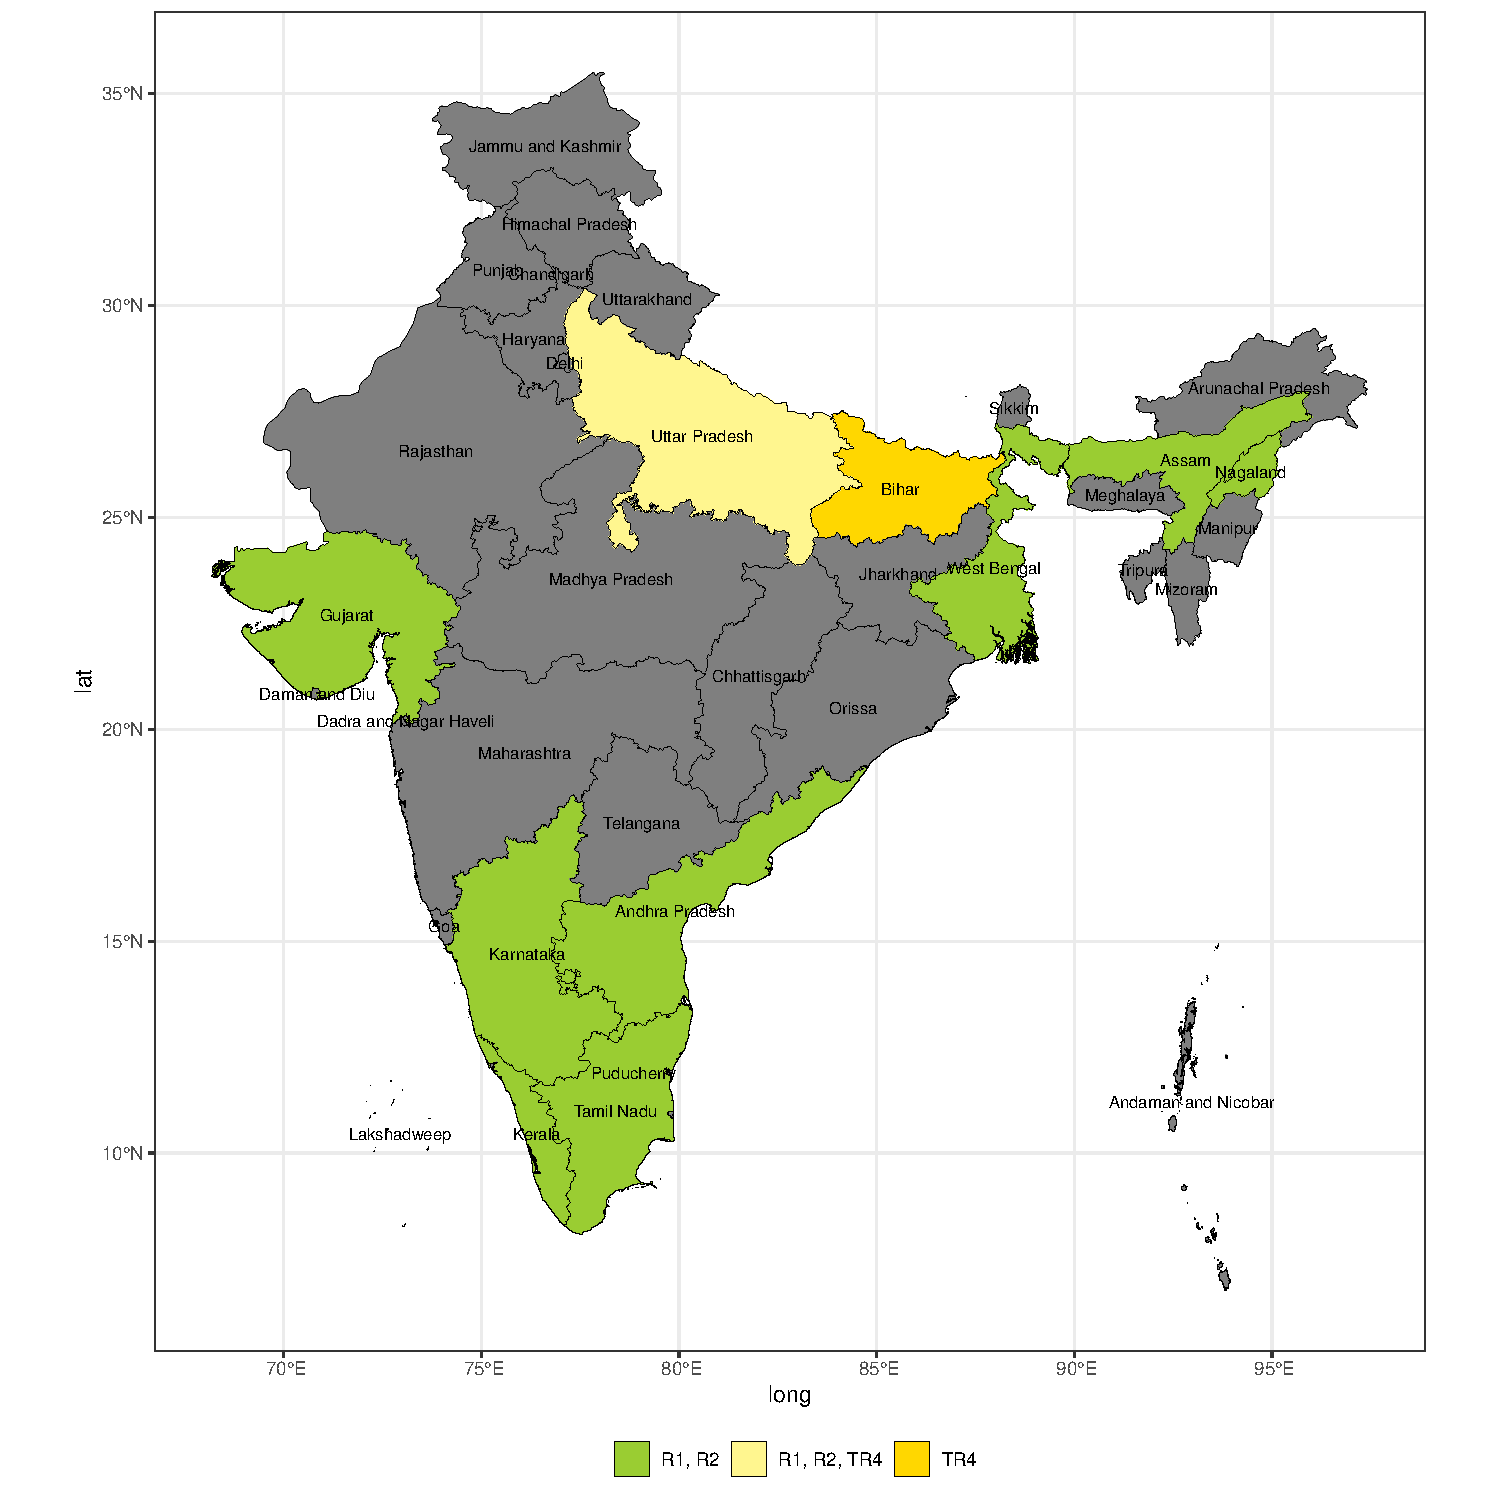
\includegraphics[width=13.5cm]{Figures/FocDis_India.pdf}
  \caption[Distribution of \textit{Fusarium oxysporum} f. sp. \textit{cubense} in India]{\textbf{ Distribution of \textit{Fusarium oxysporum} f. sp. \textit{cubense} in India}. This map shows the presence or absence by states and union territories. Areas which have not reported \ac{Focub} are shown in grey. R1: Race 1, R2: Race 2, TR4: Tropical race 4.}
  \label{fig:FocDisIndia}
\end{figure}

Collaborators at \ac{tnau}, India, assessed \ac{Focub} diversity in Tamil Nadu. Their primary goal was to explore the genetic and molecular underpinnings of banana resistance against \ac{Focub} using advanced next-generation genomics. A survey was conducted in various banana-growing areas of Tamil Nadu to record symptoms of wilt in different banana cultivars. Samples displaying symptoms of \ac{fwb}, including the \ac{Focub4} susceptible Cavendish banana variety 'Grande Naine', were collected from the field, and the pathogen was isolated and cultured in the laboratory. Among the collected samples, isolates S6, S16, S32, and SY-2, were chosen for further analysis. DNA extraction and PCR amplification were performed to confirm the identity of isolates. The isolated strains, S6, S16, and S32, exhibited severe disease symptoms when inoculated into tissue-cultured 'Grand Naine' banana plants and were classified as highly virulent. PCR amplification using \ac{r4} \textit{SIX9}-specific primers from \textcite{Carvalhais2019} confirmed that \ac{tnau} isolates were \ac{Focub} \ac{r4}, capable of infecting Cavendish banana\footnote{Results were reported by collaborators at \ac{tnau}, but data were not shown.}.

We generated genome assemblies for the \textit{Fusarium} isolates  (S6, S16, S32, and SY-2) retrieved from Cavendish banana plants and analysed genetic traits. Taxonomic identity and genetic diversity were assessed and suggest that some of the isolates collected (S16, S32, and SY-2) are members of previously unreported species in this region. Of the isolates sequenced, S6 is similar to \ac{Focub} \ac{r1} isolates but displays a \ac{Focub4} phenotype, while S16, S32, and SY-2 belong to the \acl{Ff} species complex. These classifications were supported by phylogenetic analysis, read mapping, and \ac{sixg} profiling. It is important to note, however, that bacterial contamination was detected in S6 and S32 isolates, warranting future studies to confirm this potentially novel taxon.

%%%%%%%%%%%%%%%%%%%%%%%%%%%%%%%%%%%%%%%%%%%%%
%METHODS
%%%%%%%%%%%%%%%%%%%%%%%%%%%%%%%%%%%%%%%%%%%%%
\newpage
\section{Materials and Methods}


\subsection{Extraction of genomic DNA from \textit{Fusarium} isolates carried out at \acf{tnau}}

Collaborators at \ac{tnau} maintained cultures of \textit{Fusarium} isolates (collected between 2017 and 2021 in Tamil Nadu, India) as \acf{pda} slants before transferring them to \acf{pda} plates and incubating at 28$^{\pm 2\circ}$C for four days. After 48 hours, the inoculum was introduced into 250 ml Erlenmeyer flasks containing 150 ml of \ac{pdb} and incubated at room temperature (28${\pm 2^\circ}$C) for seven days\footnote{Unfortunately, we were unable to obtain shaker model and rpm from collaborators at \acf{tnau}.}. The resulting mycelium was harvested via filtration through sterile filter paper, immediately frozen at -80$^\circ$C, and stored until DNA extraction. 

Collaborators harvested approximately 1 g of frozen mycelium and ground finely using liquid \ch{N2}. They then mixed with 5 ml of 2\% CTAB extraction buffer (containing 10 mM tris base, pH 8.0, 20 mM EDTA, pH 8.0, 1.4 M NaCl, 2\% CTAB, 0.1\% mercaptoethanol, and 0.2\% PVP) before being incubated at 65$^\circ$C for one hour. An equal volume of phenol-chloroform-isoamyl alcohol (25:24:1) mixture was added to the suspension, thoroughly mixed by vortexing, and then centrifuged at 12,000rpm at 4$^\circ$C for 5 minutes. The upper aqueous layer containing DNA (300\(\mu\)L) was carefully pipetted out, combined with 0.5 volumes of 5M NaCl and an equal volume of ice-cold isopropanol, and incubated at -20$^\circ$C for DNA precipitation for 12 hours. The precipitate was collected by centrifugation at 13,000rpm at 4$^\circ$C for 10 minutes, washed with 0.1M ammonium acetate in 70\% ethanol, and air-dried. The air-dried pellet was suspended in TE buffer (10 mM Tris, 1 mM EDTA, pH 8.0), and they determined DNA concentration spectrophotometrically.

\subsection{Library kit and protocol used for sequencing \textit{Fusarium} isolates at \ac{tnau}}

High-quality genomic DNA was prepared using TruSeq DNA Library Preparation Kit (Illumina Inc. San Diego, California, Cat FC-121-2003) for genome sequencing by collaborators at \ac{tnau}. Genomic DNA was fragmented and obtained fragments were end-repaired, A-tailed, size selected and ligated with Illumina sequencing barcode adapters. The qualified DNA libraries were pooled, and paired-end whole genome sequencing (PE 2 x 150 bp) was carried out using Illumina NovaSeq 6000 platform (M/s. Oneomics Private Limited, Trichy, India). 

\subsection{Analysis of Raw Read data from TNAU isolates}

The raw Illumina paired-end genomic reads for the \textit{Fusarium} isolates SY-2, S6, S16, and S32 were supplied by collaborators at \ac{tnau}. Isolates S6, S16 and S32 were reported to be highly virulent on Cavendish banana by collaborators (personal communication). Following FastQC (v0.11.8)
\parencite{Andrews2010} analysis, the raw reads were mapped to \ac{Focub4} UK0001 (\href{https://www.ncbi.nlm.nih.gov/datasets/genome/GCA_007994515.1/}{GCA\_007994515.1}) \parencite{Warmington2019} reference genome using Bowtie2 (v2.4.5) \parencite{Langmead2012} (for full command-line arguments and shells scripts see the \href{https://github.com/JamiePike/NewTools-Project/blob/master/docs/Assembly/AssemblyNotes.md}{GitHub Repository} referenced in section \ref{sec:chap2dataavail}). Due to poor mapping rates for some isolates, 1000 raw reads were examined from each \ac{tnau} isolate in an attempt to diagnose the issue; they were used as queries in  \ac{ncbi} \href{https://blast.ncbi.nlm.nih.gov/Blast.cgi?PROGRAM=blastn&BLAST_SPEC=GeoBlast&PAGE_TYPE=BlastSearch}{BLASTN searches} against the nr/nt database \parencite{Nih2014}. Raw reads from each isolate were also mapped to high-quality assemblies of the \ac{Focub1} isolate 160527 (\href{https://www.ncbi.nlm.nih.gov/datasets/genome/GCA_005930515.1/}{GCA\_005930515.1}) \parencite{Asai2019} and the \acl{Fs} isolate FS66 (\href{https://www.ncbi.nlm.nih.gov/datasets/genome/GCA_017165645.1/}{GCA\_017165645.1}), reported to cause leaf blight in Cavendish banana \parencite{Cui2021}. Isolates S6, S16 and S32 were also mapped to a reference quality \textit{Stenotrophomonas maltophilia} genome assembly, isolate NCTC10258 (\href{https://www.ncbi.nlm.nih.gov/datasets/genome/GCF_900475405.1/}{GCA\_900475405.1}). \textit{S. maltophilia} is a bacterial species frequently isolated from the environment and is not known to cause disease in banana and is a likely contaminant \parencite{said2021stenotrophomonas}.

\subsection{Genome Assembly and Annotation}

\subsubsection{\textit{De novo Assembly}}
A \textit{de novo} assembly was generated for each of the \ac{tnau} isolates using SPAdes (v3.14.1) \parencite{Prjibelski2020} following FastQC (v0.11.8) analysis. SPAdes is routinely used for \textit{Fusarium} genome assembly
(see: \textcite{Armitage2018, Hudson2020, Tanaka2022}). A custom Python script was developed to remove sequences with <25\% GC content from the assembly (see section \ref{sec:chap2dataavail}  \href{https://github.com/JamiePike/NewTools-Project/blob/master/bin/gcTrimmer.py}{GitHub}). As raw read data for isolates S6 and S32 contained high levels of contamination, \textit{de novo} assemblies were generated using only reads mapping to reference genomes \ac{Focub1} isolate 160527 (\href{https://www.ncbi.nlm.nih.gov/datasets/genome/GCA_005930515.1/}{GCA\_005930515.1}) \parencite{Asai2019} and \acl{Fs} isolate FS66 (\href{https://www.ncbi.nlm.nih.gov/datasets/genome/GCA_017165645.1/}{GCA\_017165645.1}) \parencite{Cui2021}, respectively. Mapped reads were determined using Bowtie2 (v2.4.5) and were extracted into separate FASTQ files using SAMtools (v1.6, using htslib v1.6) \parencite{Danecek2021}. 

\subsubsection{Contamination Analysis and Quality Assessments}
BlobTools (v1.1.1) \parencite{Laetsch2017} was used for the taxonomic partitioning of the assemblies. The \ac{tnau} assemblies were searched against the \ac{ncbi} nt/nr database using BLASTN (v2.9.0+) and the paired-end raw reads were aligned to each of the assemblies using Bowtie2 (v2.4.5). Taxonomic hits were ranked at the species level using default BlobTools (v1.1.1) settings. To extract contigs that were assigned to a non-\textit{Fusarium} genus by BlobTools (v1.1.1), the output JSON file was filtered using blobtools view, with the -r species flag. Contigs assigned to a \textit{Fusarium} species or "no-hit" were then extracted and saved in a separate text file. The BlobTools (v1.1.1) seqfilter command with the default settings was then used to extract contigs which were assigned to \textit{Fusarium} or had "no-hit".

The quality and completeness of the assembled, contaminant-filtered genomes was estimated using \ac{busco} (v5.4.6) with the hypocreales\_odb10 data set \parencite{Manni2021}. All of the raw reads were mapped back to the assemblies using Bowtie2 (v2.4.5) and a Qualimap (v2.2.2) assessment was conducted \parencite{Garcia-Alcalde2012}. Quast (v5.0.2) \parencite{Gurevich2013}  and gfastats (v1.3.6) \parencite{Formenti2022} were used to generate assembly quality statistics. 

\subsubsection{Identification of Repetitive Elements}

Repetitive elements were identified in each contaminant-filtered assembly using RepeatModeler (v2.0.4) \parencite{Flynn2020} including the -LTRStruct option. Once models had been generated, assemblies were masked iteratively with RepeatMasker (v4.1.5) \parencite{Smit2010} using the output from each round as input for the following masking step. First small, simple repeats were masked using the -noint and -xsmall options; then assemblies were masked using the default RepeatMasker (v4.1.5)  database (Dfam v3.3) \parencite{Storer2021} using the -species Fusarium option; followed by masking using the models generated by RepeatModeler (v2.0.4).

\subsubsection{Genome Annotation}
Following masking, the \ac{tnau} genomes were annotated using the MAKER pipeline (v3.01.04) \parencite{Holt2011}, including AUGUSTUS (v3.3) \parencite{Stanke2006} for \textit{ab initio} gene prediction with the “Fusarium” species option. As no RNA sequencing data were available for these isolates, homology evidence from a reference set of 387,728 proteins, from the \ac{ncbi} RefSeq nr database \parencite{Agarwala2016}, generated using the search term "Fusarium AND srcdb\_refseq[PROP]", was used. 

\subsection{Phylogenetic Analysis of \ac{tnau} isolates}\label{chap2:phylogeny}

The common \textit{Fusarium} genetic barcodes \acf{tef} and \acf{rbp2} were used to generate phylogenies \parencite{Edel-Hermann2019}. A \ac{tef} and \ac{rbp2} sequence databases were compiled using available reference sequences from the \ac{ncbi} database (see \href{https://github.com/JamiePike/NewTools-Project/tree/master/data/phylogenies}{https://github.com/JamiePike/NewTools-Project/tree/m\-aster/data/phylogenies}). Homologues of \ac{tef} and \ac{rbp2} were identified in each of our \ac{Fo} assemblies (See section:~\ref{chap3:fusariumdb}) using BLASTN (v 2.9.0+)(1e\textsuperscript{-6} cut-off). The locations of top hits were recorded, and the sequence within this region was manually examined and extracted using SAMtools (v1.15.1). The \ac{tef} and \ac{rbp2} regions from each genome were combined into a multiFASTA file for each barcode. MAFFT (v7.505) \parencite{Katoh2019} was used to construct a multiple sequence alignment, adjusting the direction according to the first sequence to ensure correct alignment and any overhanging regions were trimmed manually. IQ-TREE2 (v2.2.0.3) \parencite{Nguyen2015} was used to infer a maximum-likelihood phylogeny using the ultrafast bootstrap setting for 1000 bootstrap replicates and was visualised using iTOL \parencite{Letunic2021}. Additionally, the extracted \ac{tef} and \ac{rbp2} regions for the \ac{tnau} isolates were searched against the \ac{ncbi} nr/nt database using the  \ac{ncbi} \href{https://blast.ncbi.nlm.nih.gov/Blast.cgi?PROGRAM=blastn&BLAST_SPEC=GeoBlast&PAGE_TYPE=BlastSearch}{BLASTN suite} \parencite{Nih2014}, and the \href{https://fusarium.mycobank.org/page/Fusarium_table}{MycoBank database} \parencite{Robert2013}. 

\subsection{Identification of pathogen-specific features.}

\subsubsection{\textit{Secreted In Xylem} gene identification and phylogenetic analysis}
\label{chap1:tnauSIXgenePhylo}
To identify known \acs{Fo} effectors in the \ac{tnau} assemblies and compare the \ac{sixg} profile to other \textit{Fusaria}, reference sequences for SIX1-SIX14 used by \textcite{Czislowski2018} were downloaded from GenBank (Appendix A\ref{apx:sixgenerefs}) and homologues of each \textit{SIX} gene was identified using TBLASTN (v2.9.0+) (1e\textsuperscript{6} cut-off) in the \ac{tnau} assemblies, as well as publicly available assemblies of \ac{Focub} (n=14), \ac{Fs} (n=2), the \ac{Fo} endophyte Fo47, \ac{Fo} formae speciales \textit{cepae, conglutinans, coriandrii, lini, lycopersici,  rapae} and \textit{vasinfectum}, and \textit{F. graminearum}, which were downloaded from \href{https://www.ncbi.nlm.nih.gov/data-hub/genome/}{GenBank} following a genome search. (Table: \ref{tab:GenomeDB}). A binary data matrix indicating presence (“1”) or absence (“0”) was generated using  the TBLASTN hit data for visualisation. 

Homologues of each \ac{sixg} identified were extracted for phylogenetic analysis.  The locations of hits were recorded, and the sequence within this region was manually examined and extracted using SAMtools (v1.15.1). Sequences from each genome were added to a multiFASTA file for each \ac{sixg} and aligned with MAFFT (v7.505) \parencite{Katoh2019}, adjusting the direction according to the first sequence to ensure correct alignment. Overhanging regions were trimmed manually. IQ-TREE2 (v2.2.0.3) \parencite{Nguyen2015} was used to infer a maximum-likelihood phylogeny using the ultrafast bootstrap setting for 1000 bootstrap replicates and resulting trees were visualised using the R (v4.3.1) \parencite{R} package, ggtree (v3.10.0) \parencite{ggtree}.
\subsubsection{Identification of putative effectors}

To identify \acfp{ce} in the \ac{tnau} isolates, the predicted protein set for each isolate was filtered by size (>30aa and <450aa) and submitted to SignalP (v5.0b) \parencite{Petersen2011}. Sequences that were predicted to contain a signal peptide were passed to EffectorP (v2.0.1) \parencite{Sperschneider2018} for effector prediction. The \ac{ce} sets from each genome were then combined and clustered using CD-HIT (v4.8.1) \parencite{Fu2012} at 80\% to identify shared \acp{ce}. This approach was chosen as it adheres to the arguments for effector prediction made by \textcite{Sperschneider2015, Todd2022} (see section \ref{sec:chap2Intro}). 

%\subsubsection{Reference genome alignment and raw read mapping}

%Pathogenicity chromosomes are common among plant pathogenic \ac{Fo} \parencite{Ma2010, Fokkens2020}. As the \ac{tnau} isolate assemblies were too fragmented to characterise  pathogenic regions, \acp{mimp}, \acp{sixg}, and \acp{ce} identified using the Maei pipeline (Chapter \ref{Chap3}) were recorded in the high-quality \ac{Focub4} UK0001 and \ac{Fs} FS66 assemblies, and \ac{tnau} isolate raw reads mapped on to these assemblies using Bowtie2 (v2.4.5). Nucmer (-max match, deltafilter –g) from MUMmer (v4.0.0rc1) \parencite{Marcais2018} was used to align the ac{Focub4} UK0001 and \ac{Fs} FS66 assemblies to identify shared putative pathogenic regions between the assemblies. Circos (v0.69-8) \parencite{Krzywinski2009} was used to visualise virulence factor location and genome alignments. 

\subsection{Data and software availability}
\label{sec:chap2dataavail}

The full computational pipelines, command-line arguments as well as bash, R, and Python scripts used for all analysis outlined are available in the \href{https://github.com/JamiePike/NewTools-Project}{NewTools-Project} GitHub Repository at https://github.com/JamiePike/NewTools-Project, with supporting documentation provided in Markdown format for \href{https://github.com/JamiePike/NewTools-Project/blob/master/docs/Assembly/AssemblyNotes.md}{genome assemblies}, \href{https://github.com/JamiePike/NewTools-Project/blob/master/docs/Annotations/RepeatMaskingNotes.md}{repeat element identification and masking}, \href{https://github.com/JamiePike/NewTools-Project/blob/master/docs/Annotations/Annotations.md}{annotations}, \href{https://github.com/JamiePike/NewTools-Project/blob/master/docs/Effectors/PredicitionofCandidateEffectors.md}{\ac{ce} identification}, and \href{https://github.com/JamiePike/NewTools-Project/blob/master/docs/Phylogeny/Phylogenies.md}{phylogenetic analysis}.

%%%%%%%%%%%%%%%%%%%%%%%%%%%%%%%%%%%%%%%%%%%%%
%RESULTS
%%%%%%%%%%%%%%%%%%%%%%%%%%%%%%%%%%%%%%%%%%%%%
\newpage
\section{Results}

\subsection{Analysis of Raw Read data from TNAU isolates}
\label{sec:chap2RawReadMapping}

Mapping rates of the raw reads from isolates S6, S16, S32, and SY-2 to the \ac{Focub4} UK0001 assembly (\href{https://www.ncbi.nlm.nih.gov/datasets/genome/GCA_007994515.1/}{GCA\_007994515.1}) were 8.72\%, 53.81\%, 15.69\%, and a 54.11\%, respectively (Table ~\ref{tab:RawReadMapping}). Raw reads from each isolate were also mapped to the \ac{Focub1} 160527 assembly (\href{https://www.ncbi.nlm.nih.gov/datasets/genome/GCA_005930515.1/}{GCA\_005930515.1}), with alignment rates for all \textless 55\%. Due to the low alignment rates, unmapped reads were extracted and a random subset of 1000 reads per isolate was searched using \ac{ncbi} \href{https://blast.ncbi.nlm.nih.gov/Blast.cgi?PROGRAM=blastn&BLAST_SPEC=GeoBlast&PAGE_TYPE=BlastSearch}{web BLASTN suite} \parencite{Nih2014}, which revealed that many of the unmapped reads from these isolates were similar ($\geq90\% $ identity) to sequences from species within \ac{FFSC}. Further, isolates S6 and S32 displayed signs of possible bacterial contamination, with raw reads displaying $ \geq90\% $ identity to sequences from \textit{Stenotrophomonas} species, particularly \textit{S. maltophilia}. 

All raw reads from isolates S6, S16, S32, and SY-2 were mapped to a \acf{Fs} reference assembly, isolate FS66 (\href{https://www.ncbi.nlm.nih.gov/datasets/genome/GCA_017165645.1/}{GCA\_017165645.1}). \ac{Fs} is a member of the \acf{FFSC} and FS66 has recently been reported to cause leaf blight symptoms in banana \parencite{Cui2021}. Raw reads from isolates S6 and S32 had a 5.24\% and 22.49\% mapping rate to the \ac{Fs} reference, respectively, whereas 68.65\% of the raw reads from isolate S16 and 93.96\% of the raw reads from the SY-2 isolate mapped to the \ac{Fs} reference assembly (Table ~\ref{tab:RawReadMapping}). Isolates S6, S16, and S32 were also mapped to a reference-quality \textit{S. maltophilia} genome assembly (\href{https://www.ncbi.nlm.nih.gov/datasets/genome/GCF_900475405.1/}{GCA\_900475405.1}, isolate NCTC10258). Approximately 50\% of raw reads from isolates S6 and S32 mapped to the \textit{S. maltophilia} reference, whereas raw reads from isolate S16 only had a 0.01\% mapping rate to the \textit{S. maltophilia} reference. Further, the raw S6 and S32 reads show a similar GC\% to the \textit{S. maltophilia} reference genome (S6=63\%, S32=61\%, NCTC10258=66.5\%).

\bigskip
% Please add the following required packages to your document preamble:
% \usepackage{booktabs}
% \usepackage{multirow}
% \usepackage{graphicx}
\begin{table}[h!]
\caption[Overall alignment rate of all raw reads from each TNAU isolates to fungal and bacterial reference species]{{\textbf{Overall alignment rate of all raw reads from each TNAU isolates to fungal and bacterial reference species.}} Overall alignment rate determined by Bowtie2 (version 2.4.5). Reference assemblies were downloaded from GenBank: \ac{Focub4} isolate UK0001 (\href{https://www.ncbi.nlm.nih.gov/datasets/genome/GCA_007994515.1/}{GCA\_007994515.1}), \ac{Focub1} isolate 160527 (\href{https://www.ncbi.nlm.nih.gov/datasets/genome/GCA_005930515.1/}{GCA\_005930515.1}), \textit{Fusairum sacchari} isolate FS66 (\href{https://www.ncbi.nlm.nih.gov/datasets/genome/GCA_017165645.1/}{GCA\_017165645.1}), \textit{Stenotrophomonas maltophilia} isolate NCTC10258 (\href{https://www.ncbi.nlm.nih.gov/datasets/genome/GCF_900475405.1/}{GCA\_900475405.1}).}
\label{tab:RawReadMapping}
\centering
\resizebox{\textwidth}{!}{%
\begin{tabular}{cccccc}
\hline
\multirow{2}{*}{\textbf{Reference Species}} & \multirow{2}{*}{\textbf{Strain}} & \multicolumn{4}{c}{\textbf{BOWTIE2 Alignment Rate}} \\ \cline{3-6} 
 &  & \textbf{S6} & \textbf{S16} & \textbf{S32} & \textbf{SY-2} \\ \cline{1-2}
\textit{Fo.} f. sp. \textit{cubense} (TR4) & UK0001 & 8.72\% & 53.81\% & 15.69\% & 54.11\% \\
\textit{Fo.} f. sp. \textit{cubense} (R1) & 160527 & 9.90\% & 53.67\% & 15.51\% & 54.02\% \\
\textit{F. sacchari} & FS66 & 5.24\% & 68.65\% & 22.49\% & 93.96\% \\
\textit{Stenotrophomonas maltophilia} & NCTC10258 & 49.32\% & 0.01\% & 53.93\% & -- \\ \hline
\end{tabular}%
}
\end{table}

\subsection{Contamination Analysis and \textit{de novo} Genome Assembly}

As <55\% of raw reads from the \ac{tnau} isolates aligned to the \ac{Focub1} and \ac{Focub4} reference assemblies, the \ac{tnau} genomes were assembled \textit{de novo}. All raw reads were used for the S16 and SY-2 genome assemblies, and due to the level of \textit{S. maltophilia} contamination (Table \ref{tab:RawReadMapping}), S6 and S32 \textit{de novo} genome assemblies were generated using only reads aligning to the reference genomes \ac{Focub1} isolate 160527 (\href{https://www.ncbi.nlm.nih.gov/datasets/genome/GCA_005930515.1/}{GCA\_005930515.1}) \parencite{Asai2019} and \ac{Fs} isolate FS66 (\href{https://www.ncbi.nlm.nih.gov/datasets/genome/GCA_017165645.1/}{GCA\_017165645.1}) \parencite{Cui2021}, respectively. Following assembly, low-GC contigs  (\textless 25\%) were removed from the SY-2 and S16 assemblies (this was not performed for S6 and S32, as assembly GC content followed a normal distribution, see appendix A\ref{fig:tnuaGCplots}), reducing the total number of contigs from 1,548 to 441 in the SY-2 assembly (2.01 Mb) and 1,666 to 768 in the S16 assembly (1.85 Mb).  

A BlobTools (v1.1.1) analysis was used to identify any potential contaminant contigs after removing the low GC contigs. Although \textit{Fusarium} species accounted for the majority of the \ac{ncbi} nt database hits for the SY-2 genome assembly, with 365 contigs assigned to \ac{Ff}, some potential contamination from \textit{Musa} species was identified, with 14 contigs assigned to \textit{Musa balbisiana} and one assigned to \textit{Musa textilis} (Figure \ref{fig:SY-2:BlobTools}). The S6, S16, and S32 genome assemblies contained hits from only \textit{Fusarium} species or had no species allocated (no-hit) and no other genera were identified. For S16 and S32, the majority of contigs were assigned to \acf{Ff} (Figure \ref{fig:S16:BlobTools}, \ref{fig:S32:BlobTools}), whereas the  S6 genome assembly contained contigs assigned to \ac{Ff} and \ac{Fo}, although 2,301 contigs had no hits (Figure \ref{fig:S6:BlobTools}).  

%%%%%%%%%%%%%%%%%%%%%%%%%%
%%%%% SY-2 BlobTools %%%%%
%%%%%%%%%%%%%%%%%%%%%%%%%%
\begin{figure}[hp!]
    \centering
    \begin{subfigure}[]{0.99\textwidth}
        \centering
        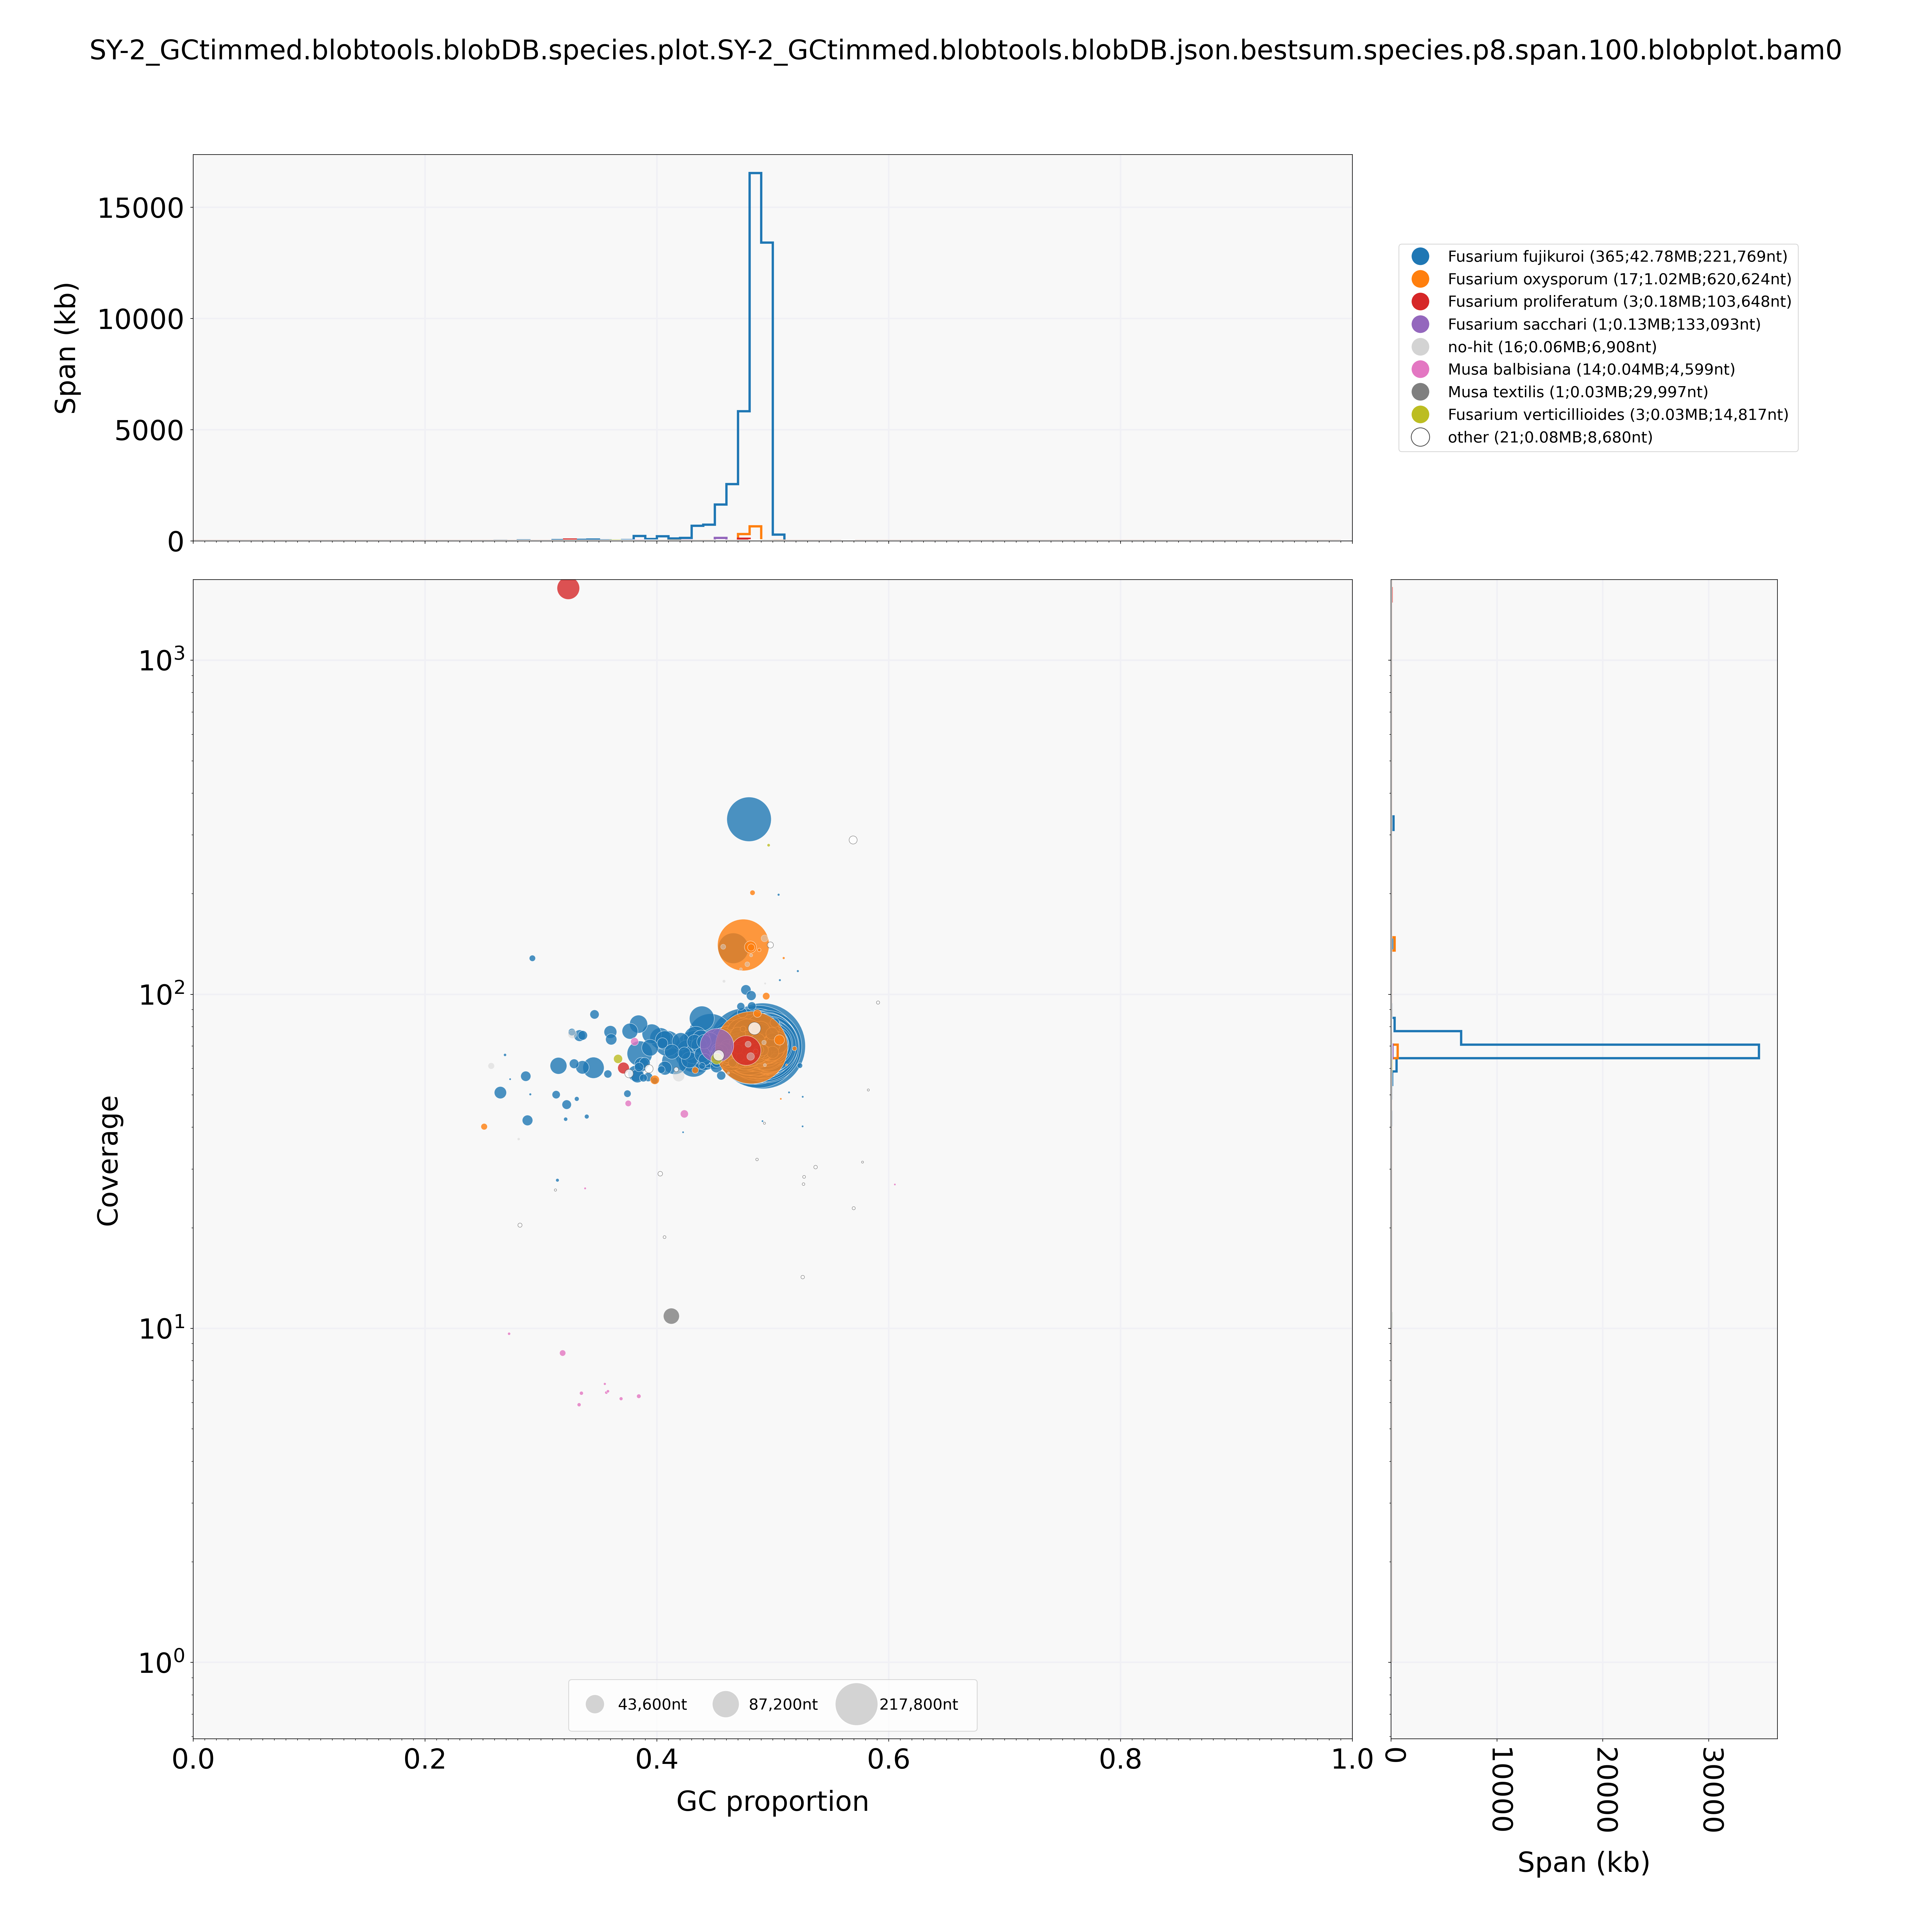
\includegraphics[width=\textwidth]{Appendices/SY-2_GCtimmed.blobtools.blobDB.species.plot.SY-2_GCtimmed.blobtools.blobDB.json.bestsum.species.p8.span.100.blobplot.bam0.png}
        \caption{}
        \label{fig:BlobPlot-SY-2}
    \end{subfigure}
    \begin{subfigure}[]{0.9\textwidth}
        \centering
        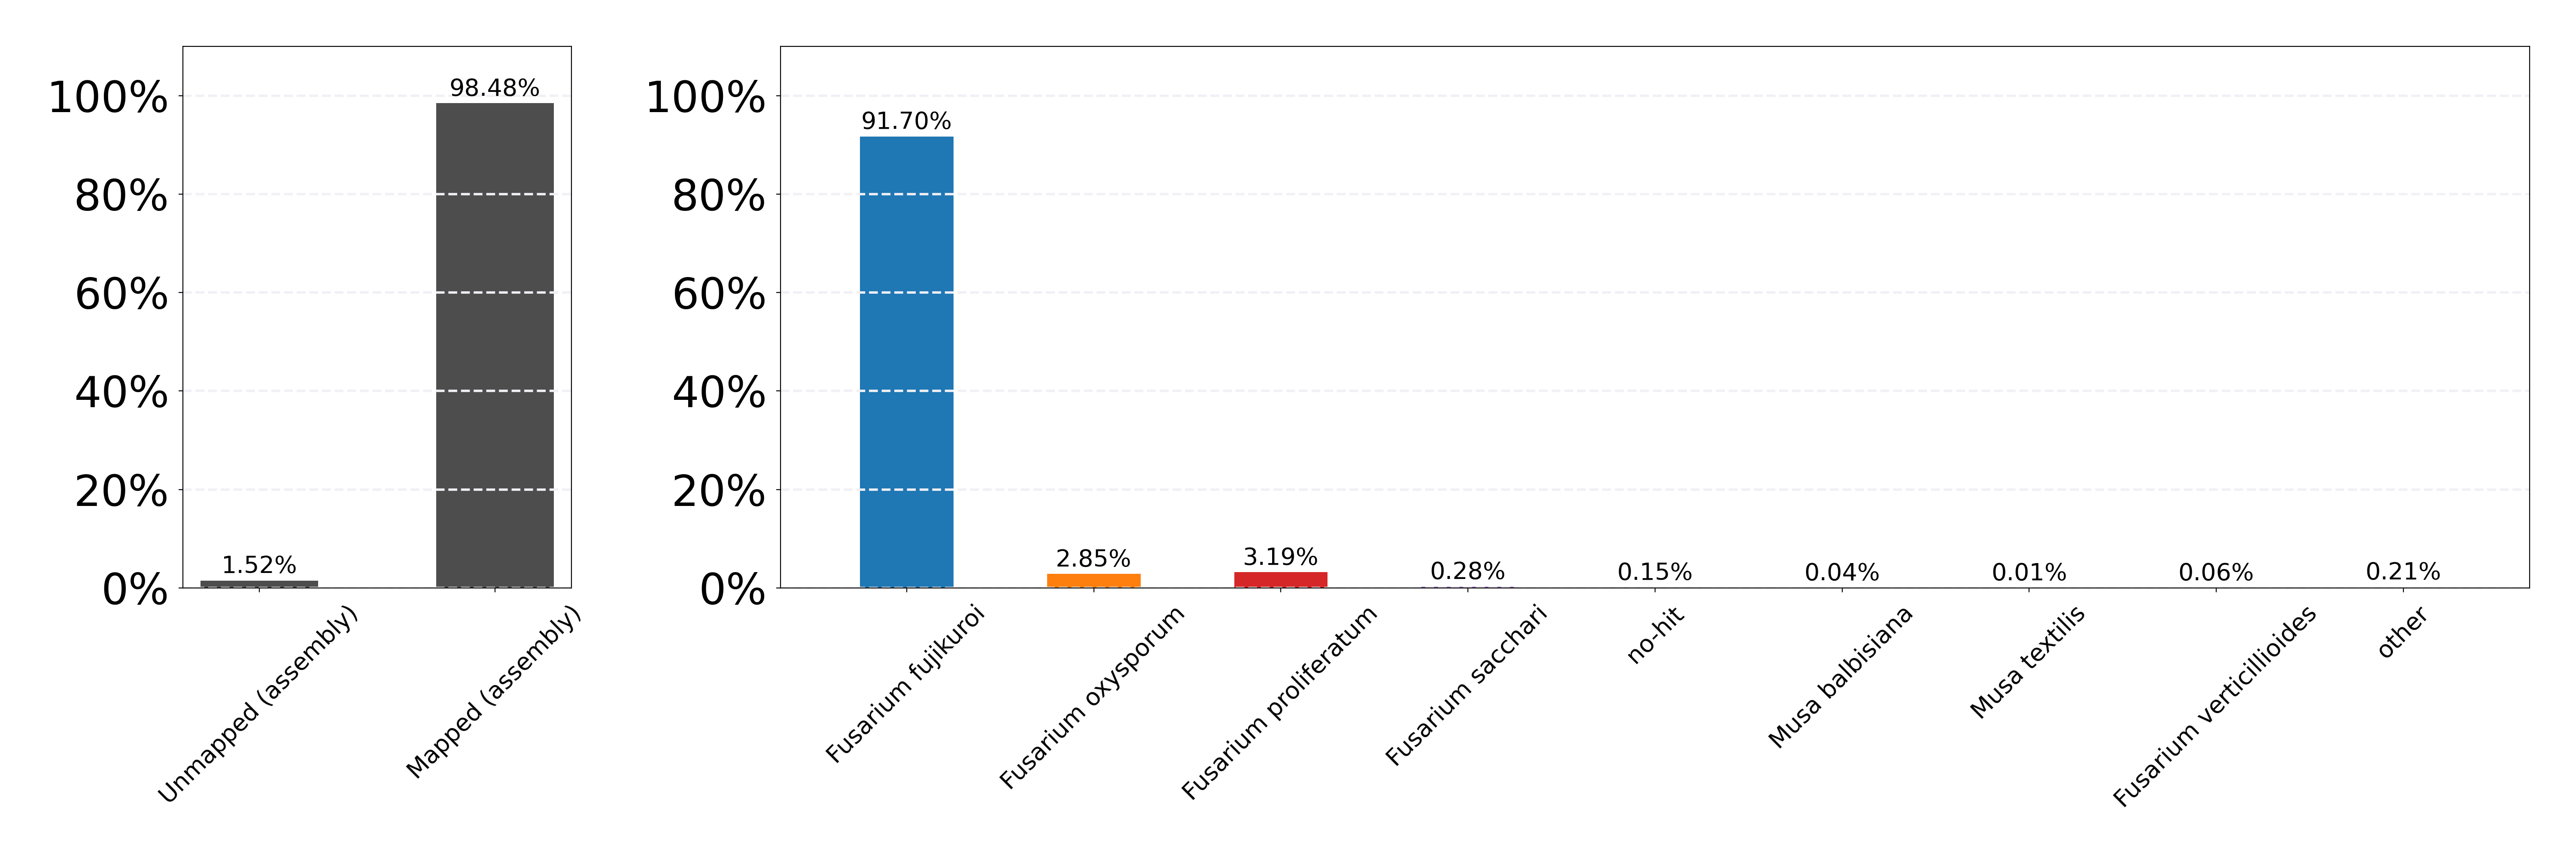
\includegraphics[width=\textwidth]{Appendices/SY-2_GCtimmed.blobtools.blobDB.species.plot.SY-2_GCtimmed.blobtools.blobDB.json.bestsum.species.p8.span.100.blobplot.read_cov.bam0.png}
        \caption{}
        \label{fig:BlobPlot_readcov-SY-2}
    \end{subfigure}
    \caption[BlobTools visualisations of the SY-2 assembly]{\textbf{BlobTools visualisations of the SY-2 assembly.}
        \textbf{\subref{fig:BlobPlot-SY-2})} BlobPlot of SY-2. Sequences in the assembly are depicted as circles, with diameter proportional to sequence length and coloured by taxonomic annotation based on BLASTN (v2.9.0+) of NCBI nt database.
        \textbf{\subref{fig:BlobPlot_readcov-SY-2})} Read coverage plot of the SY-2 assembly. Mapped reads are shown by taxonomic group at the rank of species.}
        \label{fig:SY-2:BlobTools}
\end{figure}

%%%%%%%%%%%%%%%%%%%%%%%%%%
%%%%% S16 BlobTools %%%%%%
%%%%%%%%%%%%%%%%%%%%%%%%%%
\begin{figure}[hp!]
    \centering
    \begin{subfigure}[]{0.99\textwidth}
        \centering
        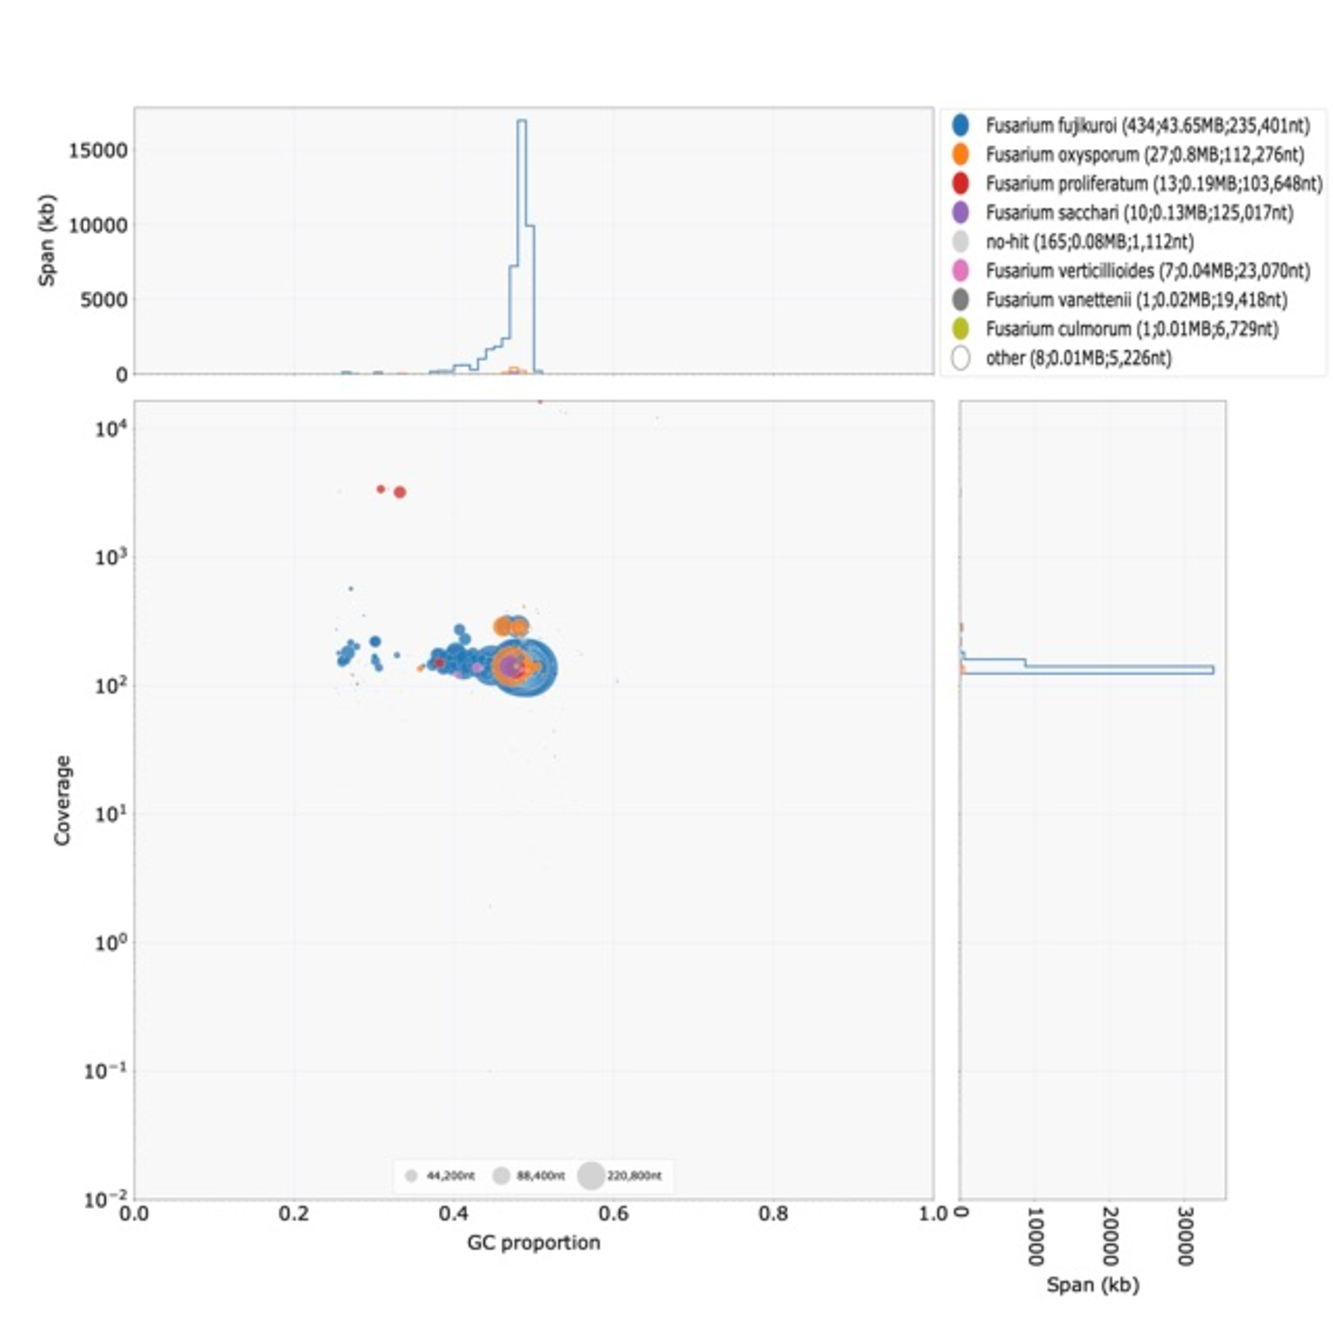
\includegraphics[width=\textwidth]{Figures/TNAU_S16.species.blobplot.pdf}
        \caption{}
        \label{fig:BlobPlot-S16}
    \end{subfigure}
    \begin{subfigure}[]{0.9\textwidth}
        \centering
        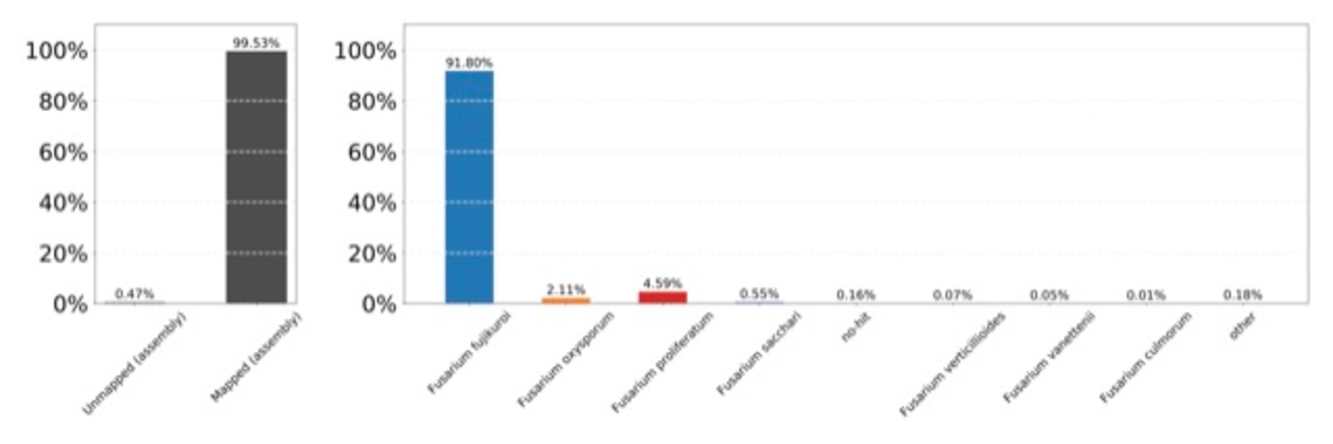
\includegraphics[width=\textwidth]{Figures/TNAU_S16.blobtools.blobDB.json.bestsum.species.p8.span.100.blobplot.read_cov.bam0.pdf}
        \caption{}
        \label{fig:BlobPlot_readcov-S16}
    \end{subfigure}
    \caption[BlobTools visualisations of the S16 assembly]{\textbf{BlobTools visualisations of the S16 assembly.}
        \subref{fig:BlobPlot-S16})\textbf{ BlobPlot of S16. Sequences in }the assembly are depicted as circles, with diameter proportional to sequence length and coloured by taxonomic annotation based on BLASTN (v2.9.0+) of NCBI nt database.
        \textbf{\subref{fig:BlobPlot_readcov-S16}}) Read coverage plot of the S16 assembly. Mapped reads are shown by taxonomic group at the rank of species.}
        \label{fig:S16:BlobTools}
\end{figure}
%%%%%%%%%%%%%%%%%%%%%%%%%%
%%%%% S32 BlobTools %%%%%%
%%%%%%%%%%%%%%%%%%%%%%%%%%
\begin{figure}[hp!]
    \centering
    \begin{subfigure}[]{0.99\textwidth}
        \centering
        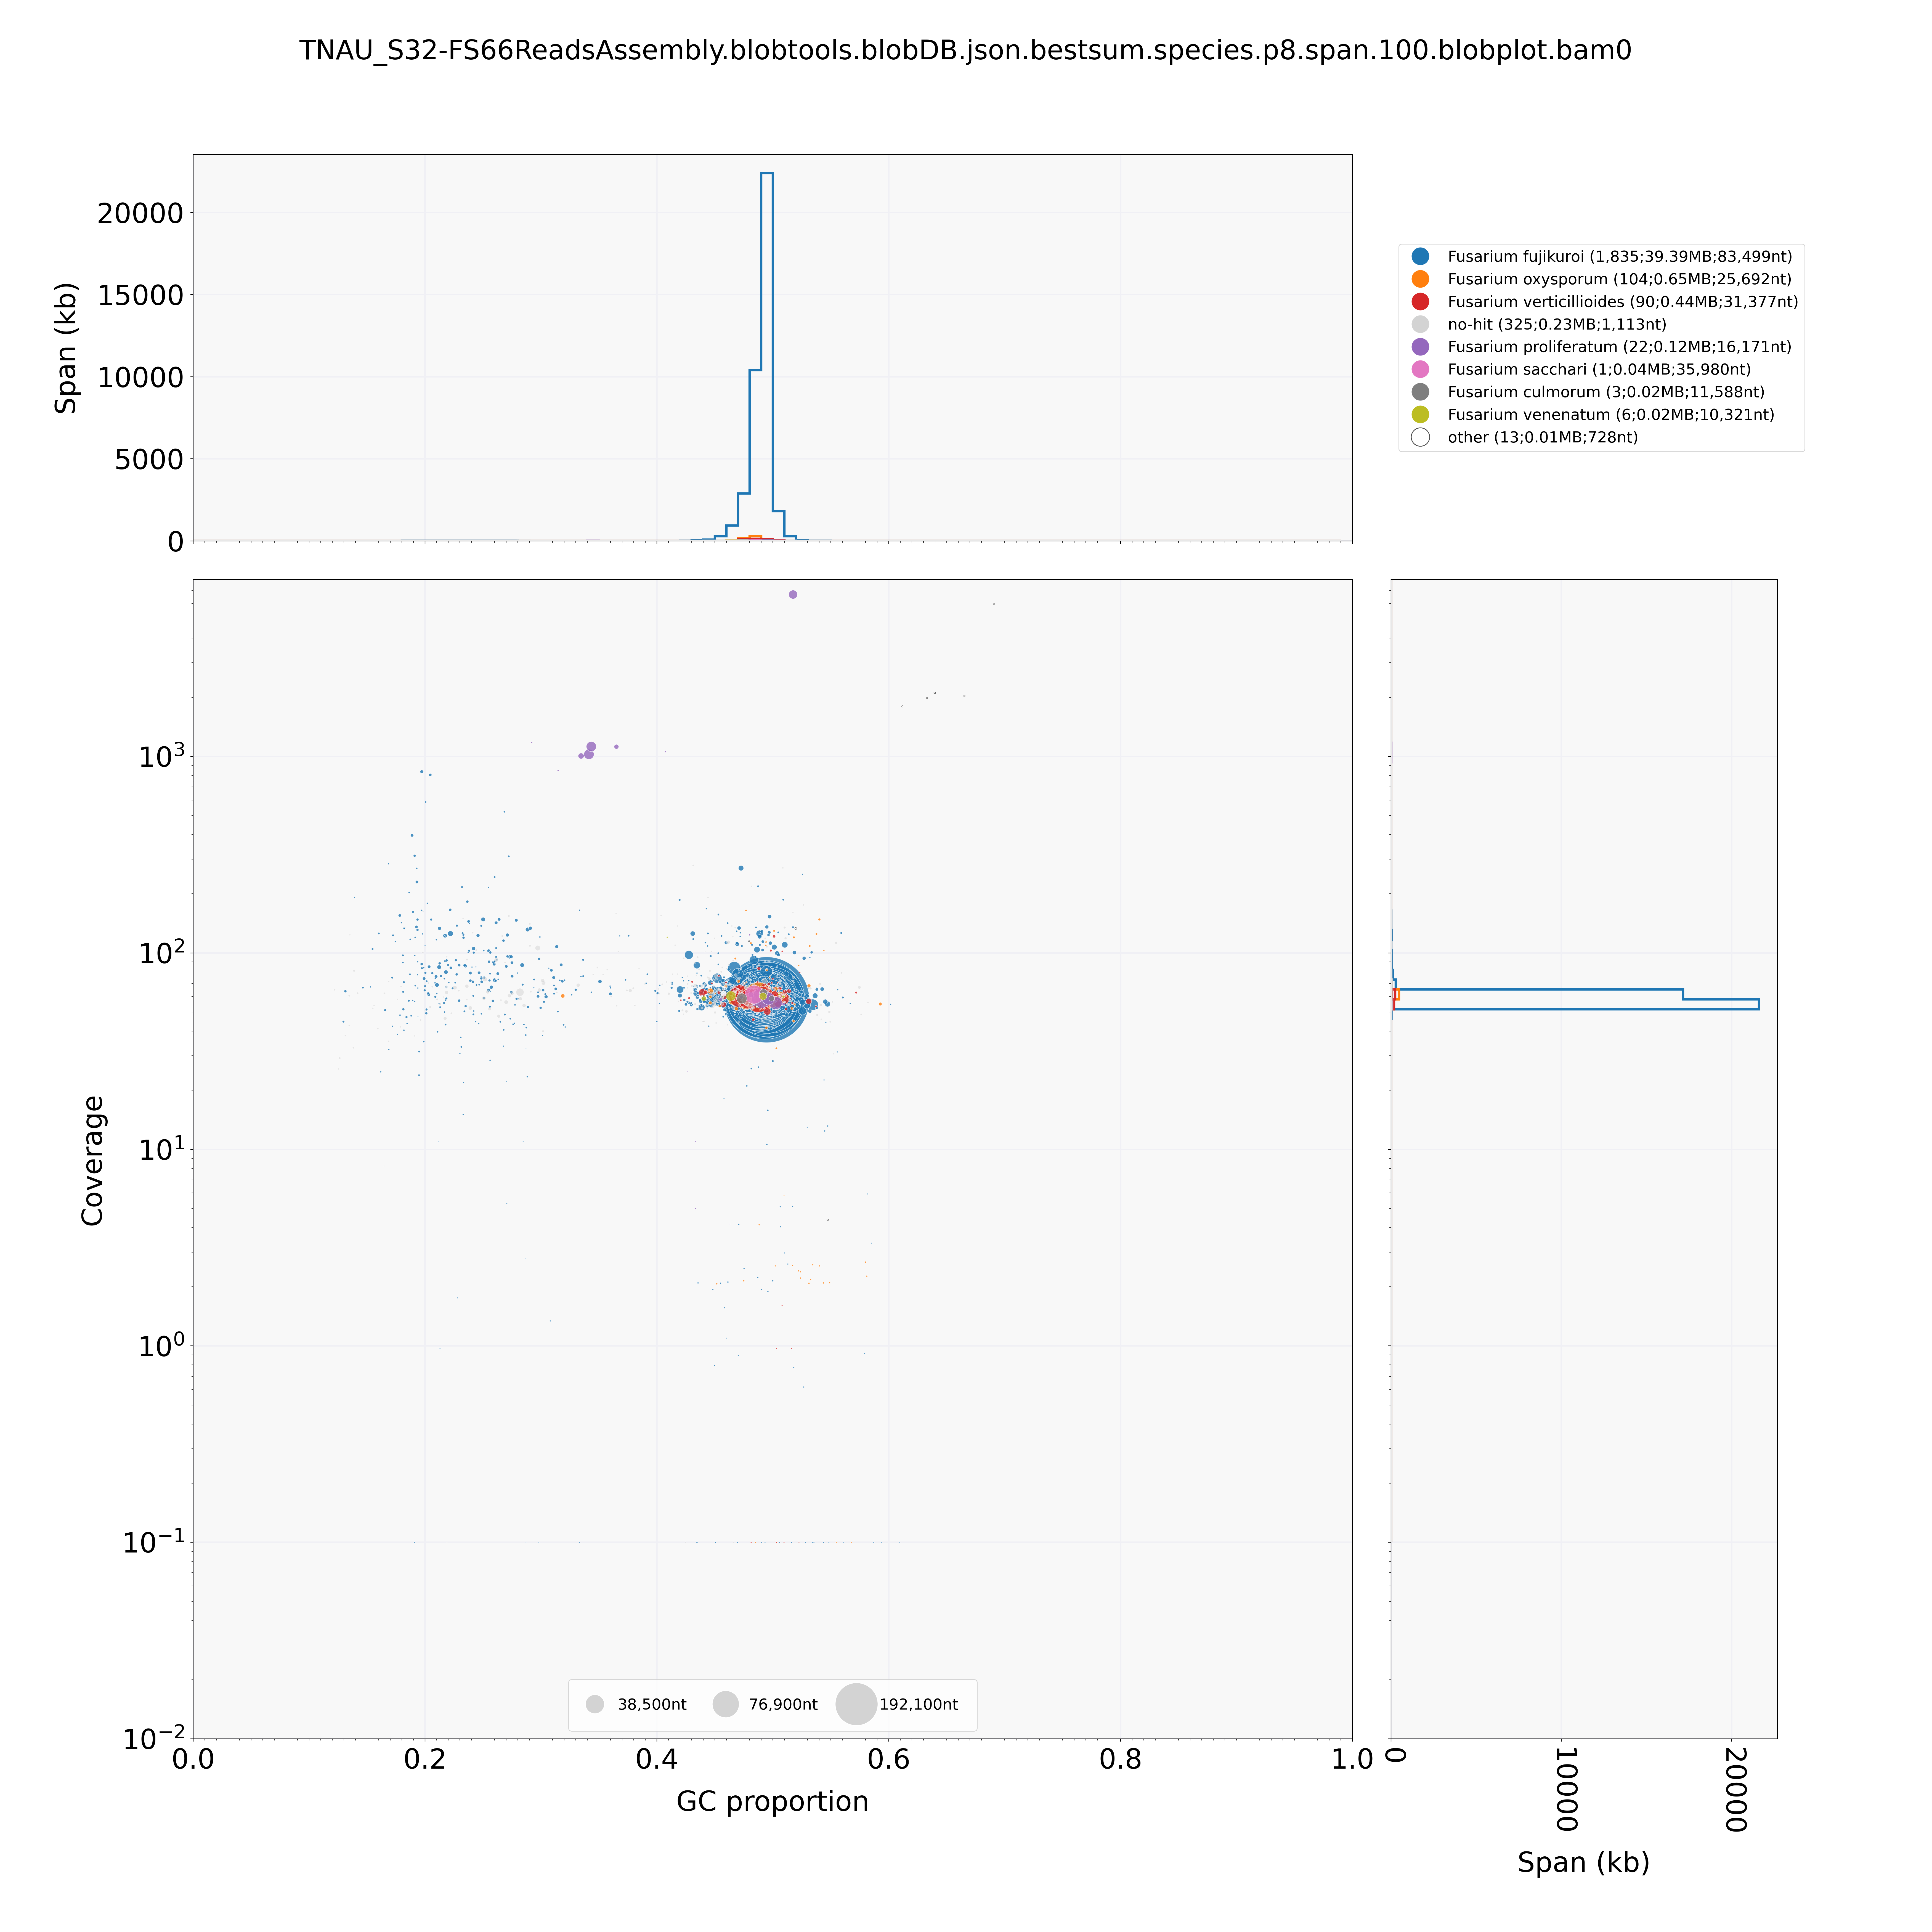
\includegraphics[width=\textwidth]{Appendices/TNAU_S32-FS66ReadsAssembly.blobtools.blobDB.json.bestsum.species.p8.span.100.blobplot.bam0.png}
        \caption{}
        \label{fig:BlobPlot-S32}
    \end{subfigure}
    \begin{subfigure}[]{0.9\textwidth}
        \centering
        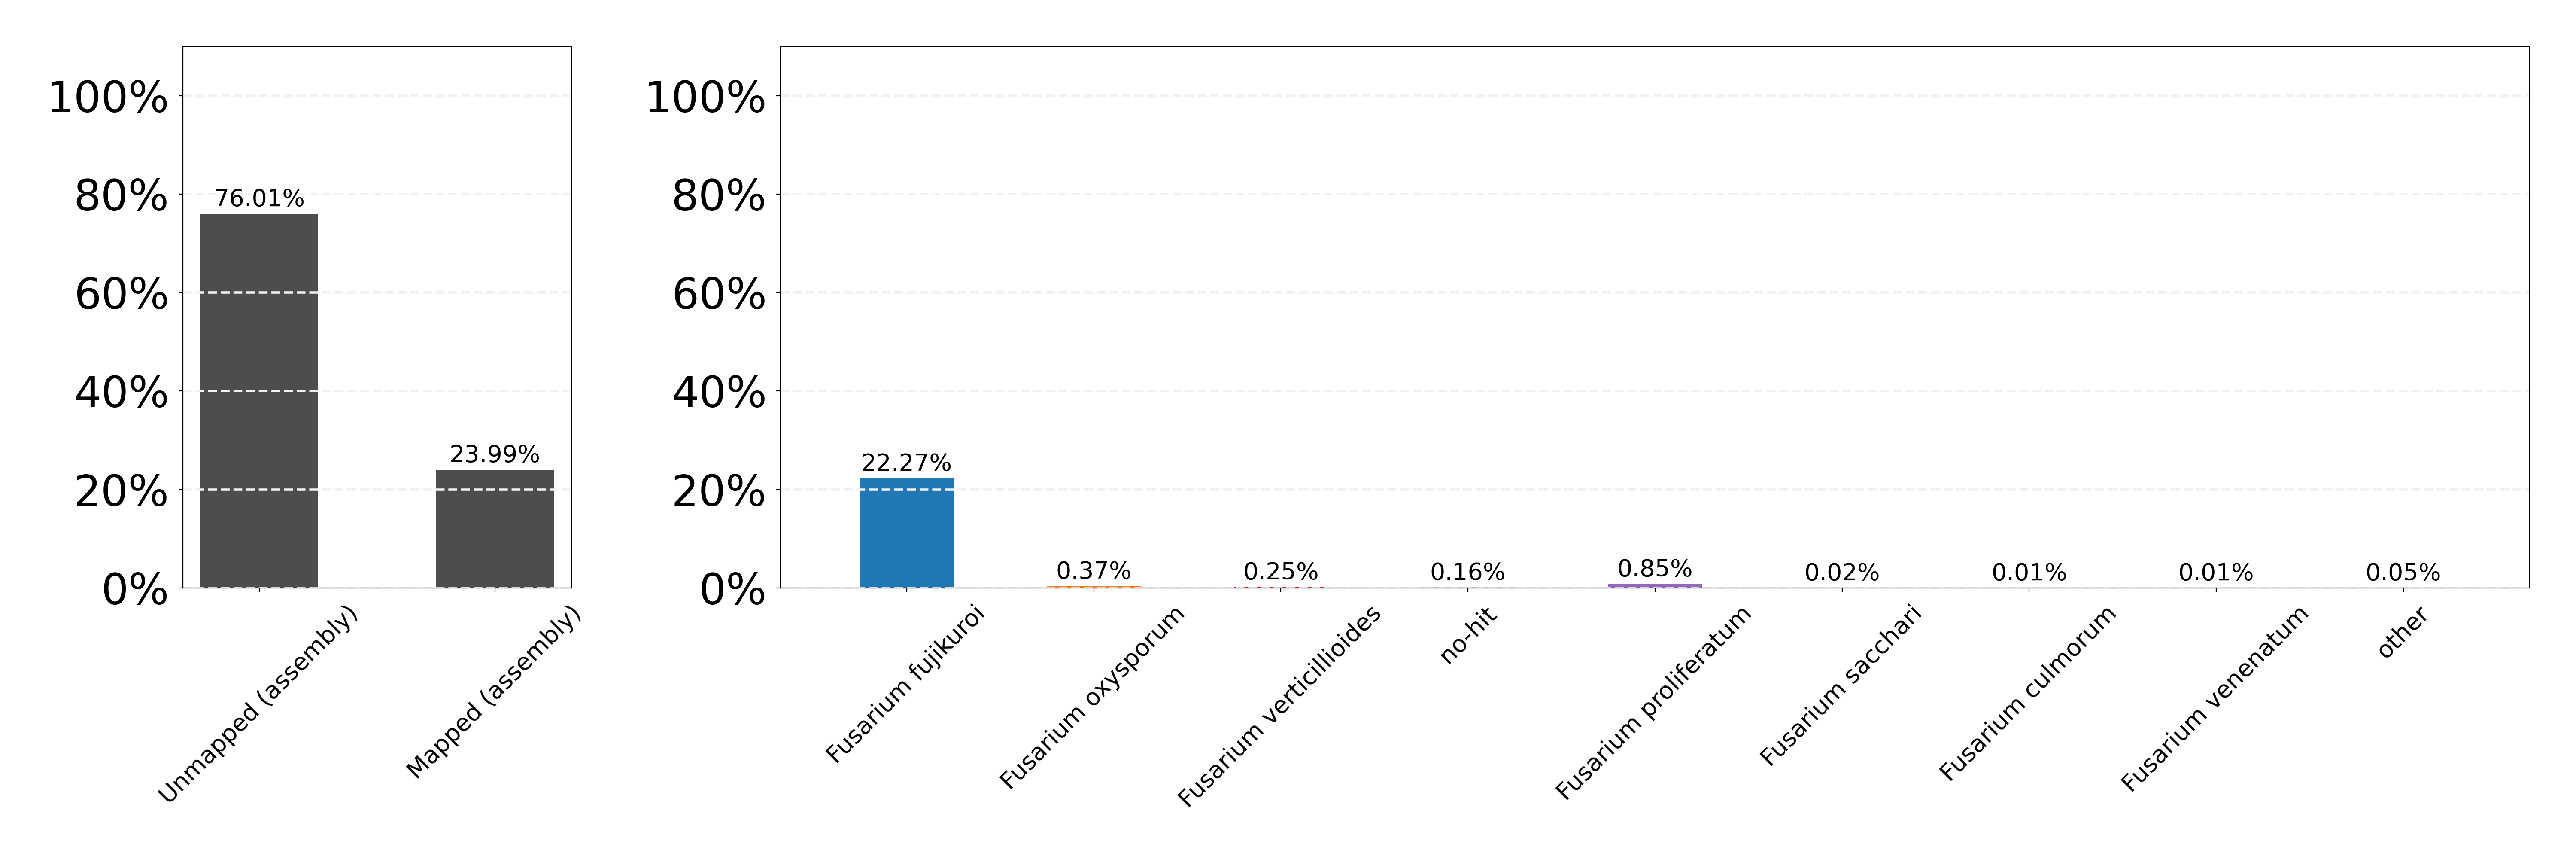
\includegraphics[width=\textwidth]{Appendices/TNAU_S32-FS66ReadsAssembly.blobtools.blobDB.json.bestsum.species.p8.span.100.blobplot.read_cov.bam0.png}
        \caption{}
        \label{fig:BlobPlot_readcov-S32}
    \end{subfigure}
    \caption[BlobTools visualisations of the S32 assembly]{\textbf{BlobTools visualisations of the S32 assembly.}
        \textbf{\subref{fig:BlobPlot-S32}) }BlobPlot of S32. Sequences in the assembly are depicted as circles, with diameter proportional to sequence length and coloured by taxonomic annotation based on BLASTN (v2.9.0+) of NCBI nt database.
        \textbf{\subref{fig:BlobPlot_readcov-S32})} Read coverage plot of the S16 assembly. Mapped reads are shown by taxonomic group at the rank of species.}
        \label{fig:S32:BlobTools}
\end{figure}
%%%%%%%%%%%%%%%%%%%%%%%%%%
%%%%%% S6 BlobTools %%%%%%
%%%%%%%%%%%%%%%%%%%%%%%%%%
\begin{figure}[hp!]
    \centering
    \begin{subfigure}[]{0.99\textwidth}
        \centering
        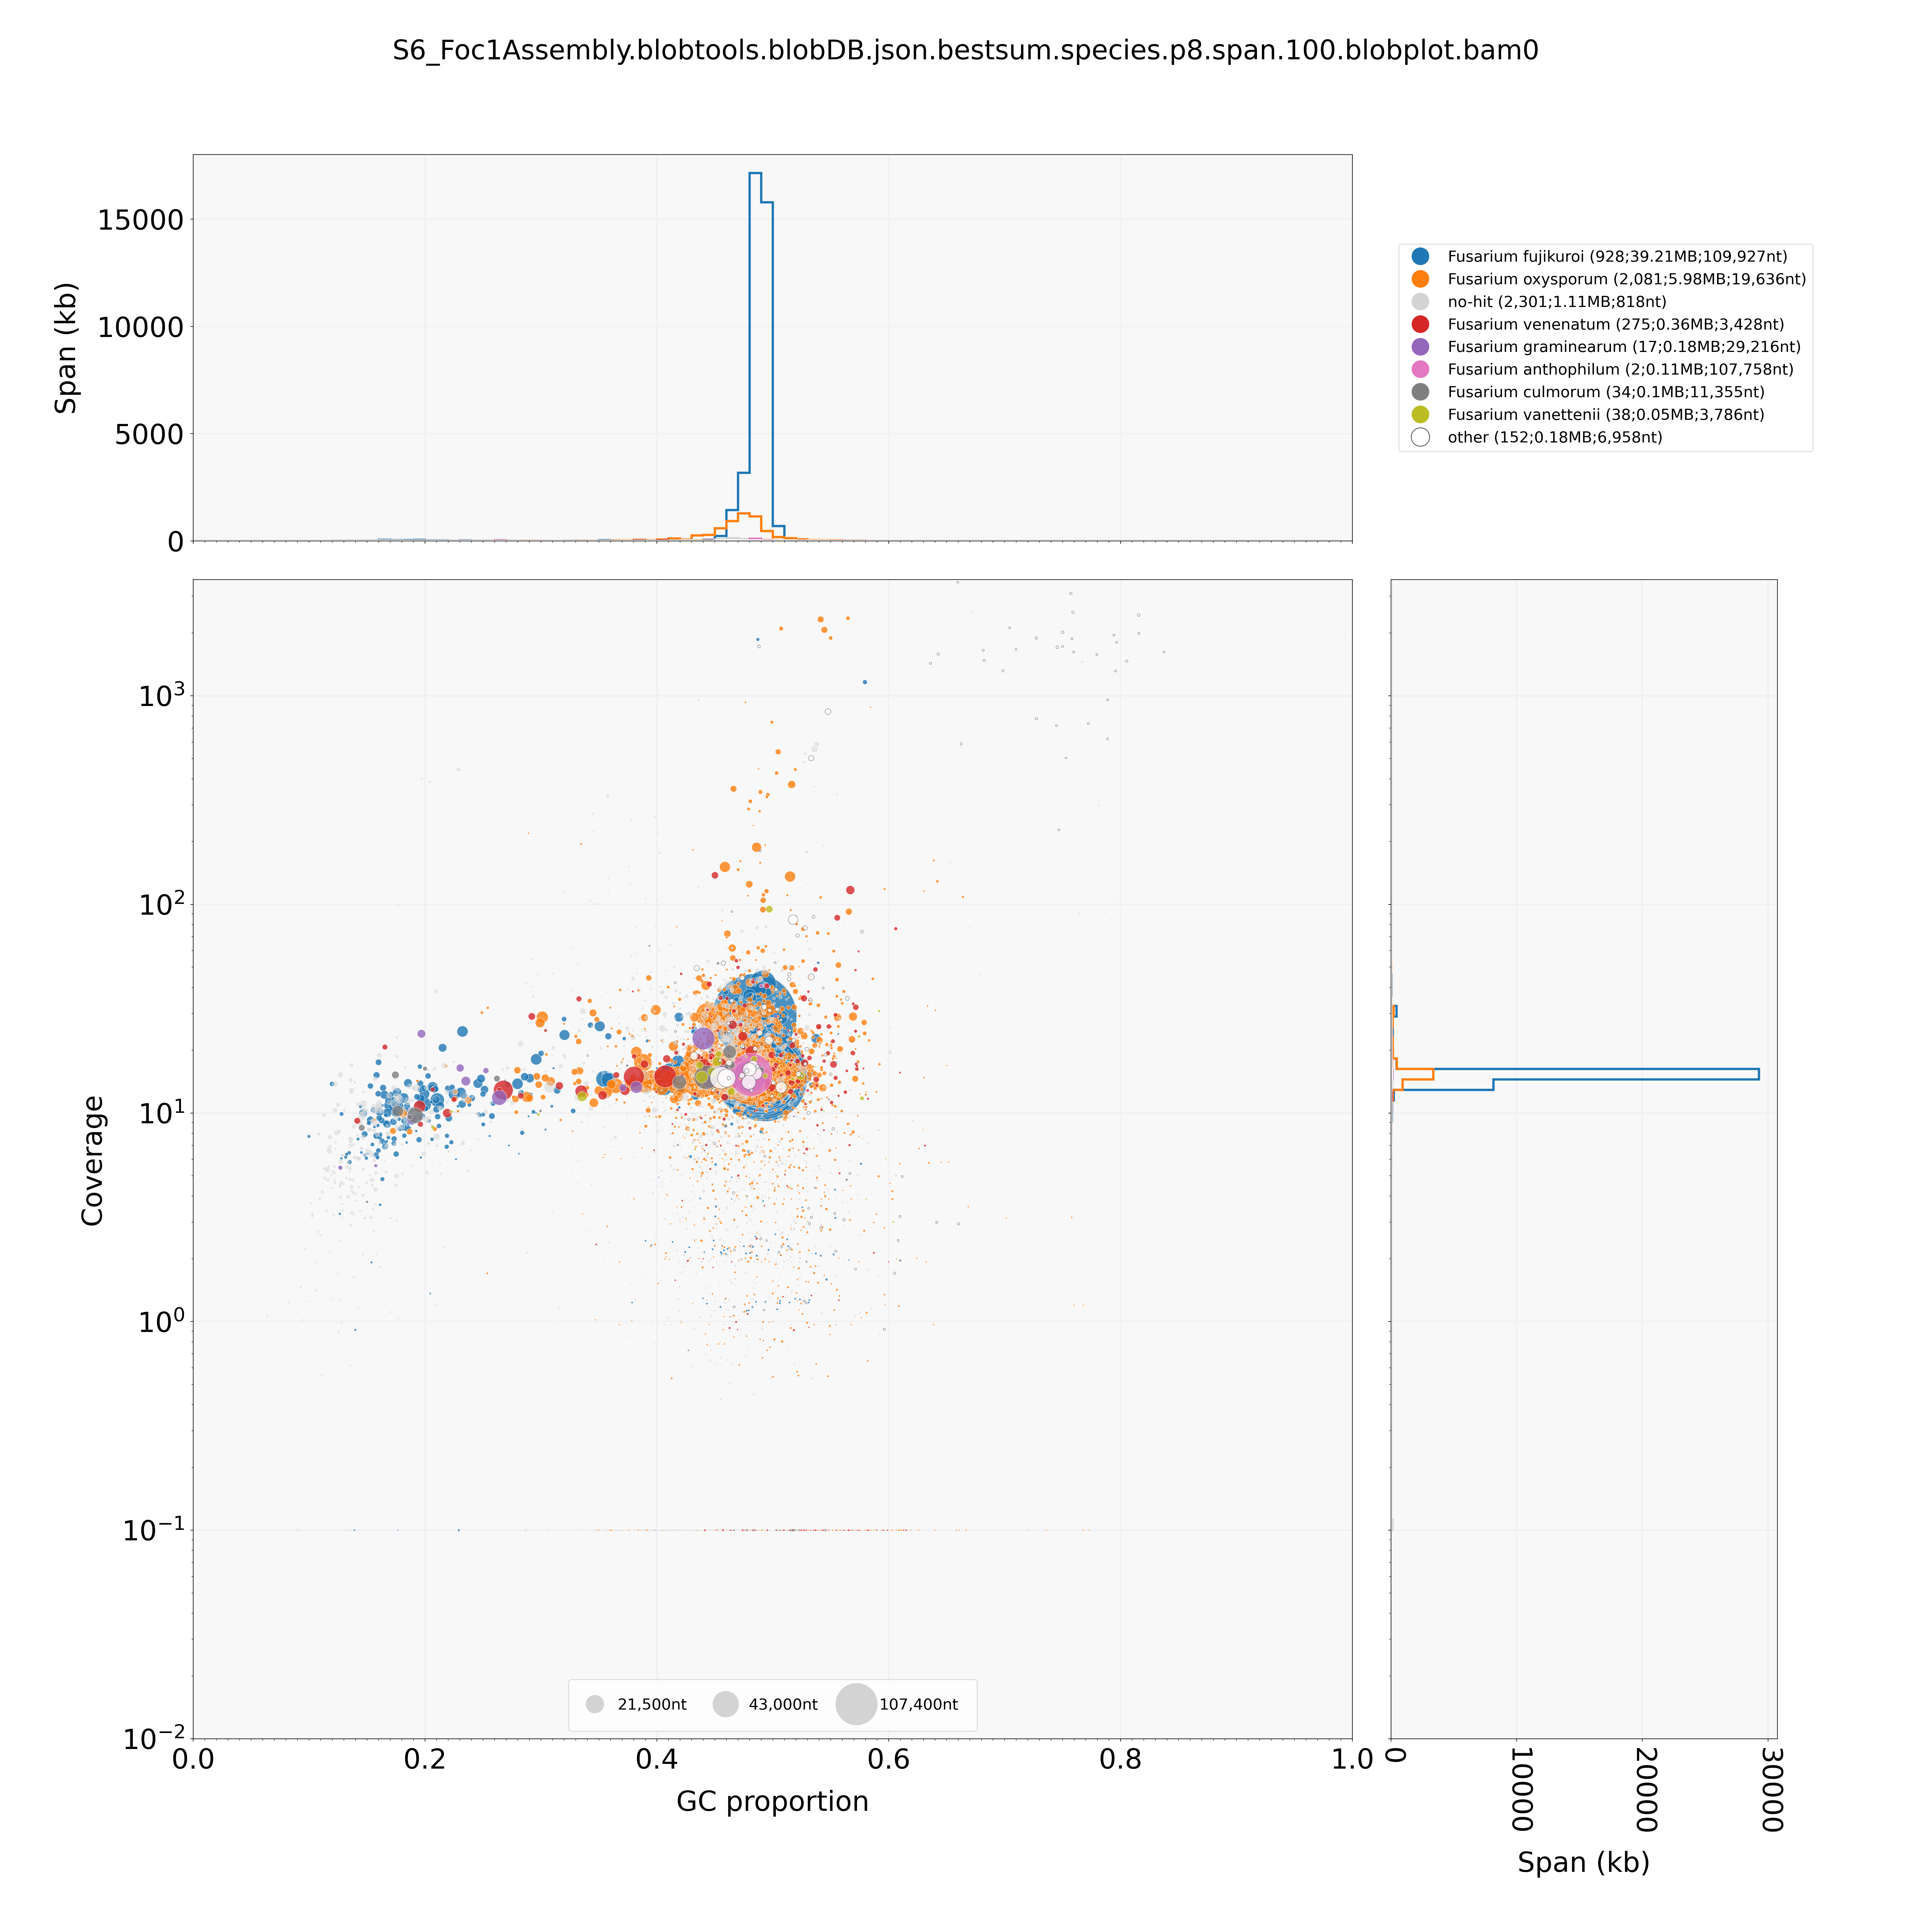
\includegraphics[width=\textwidth]{Appendices/S6_Foc1Assembly.blobtools.blobDB.json.bestsum.species.p8.span.100.blobplot.bam0.png}
        \caption{}
        \label{fig:BlobPlot-S6}
    \end{subfigure}
    \begin{subfigure}[]{0.9\textwidth}
        \centering
        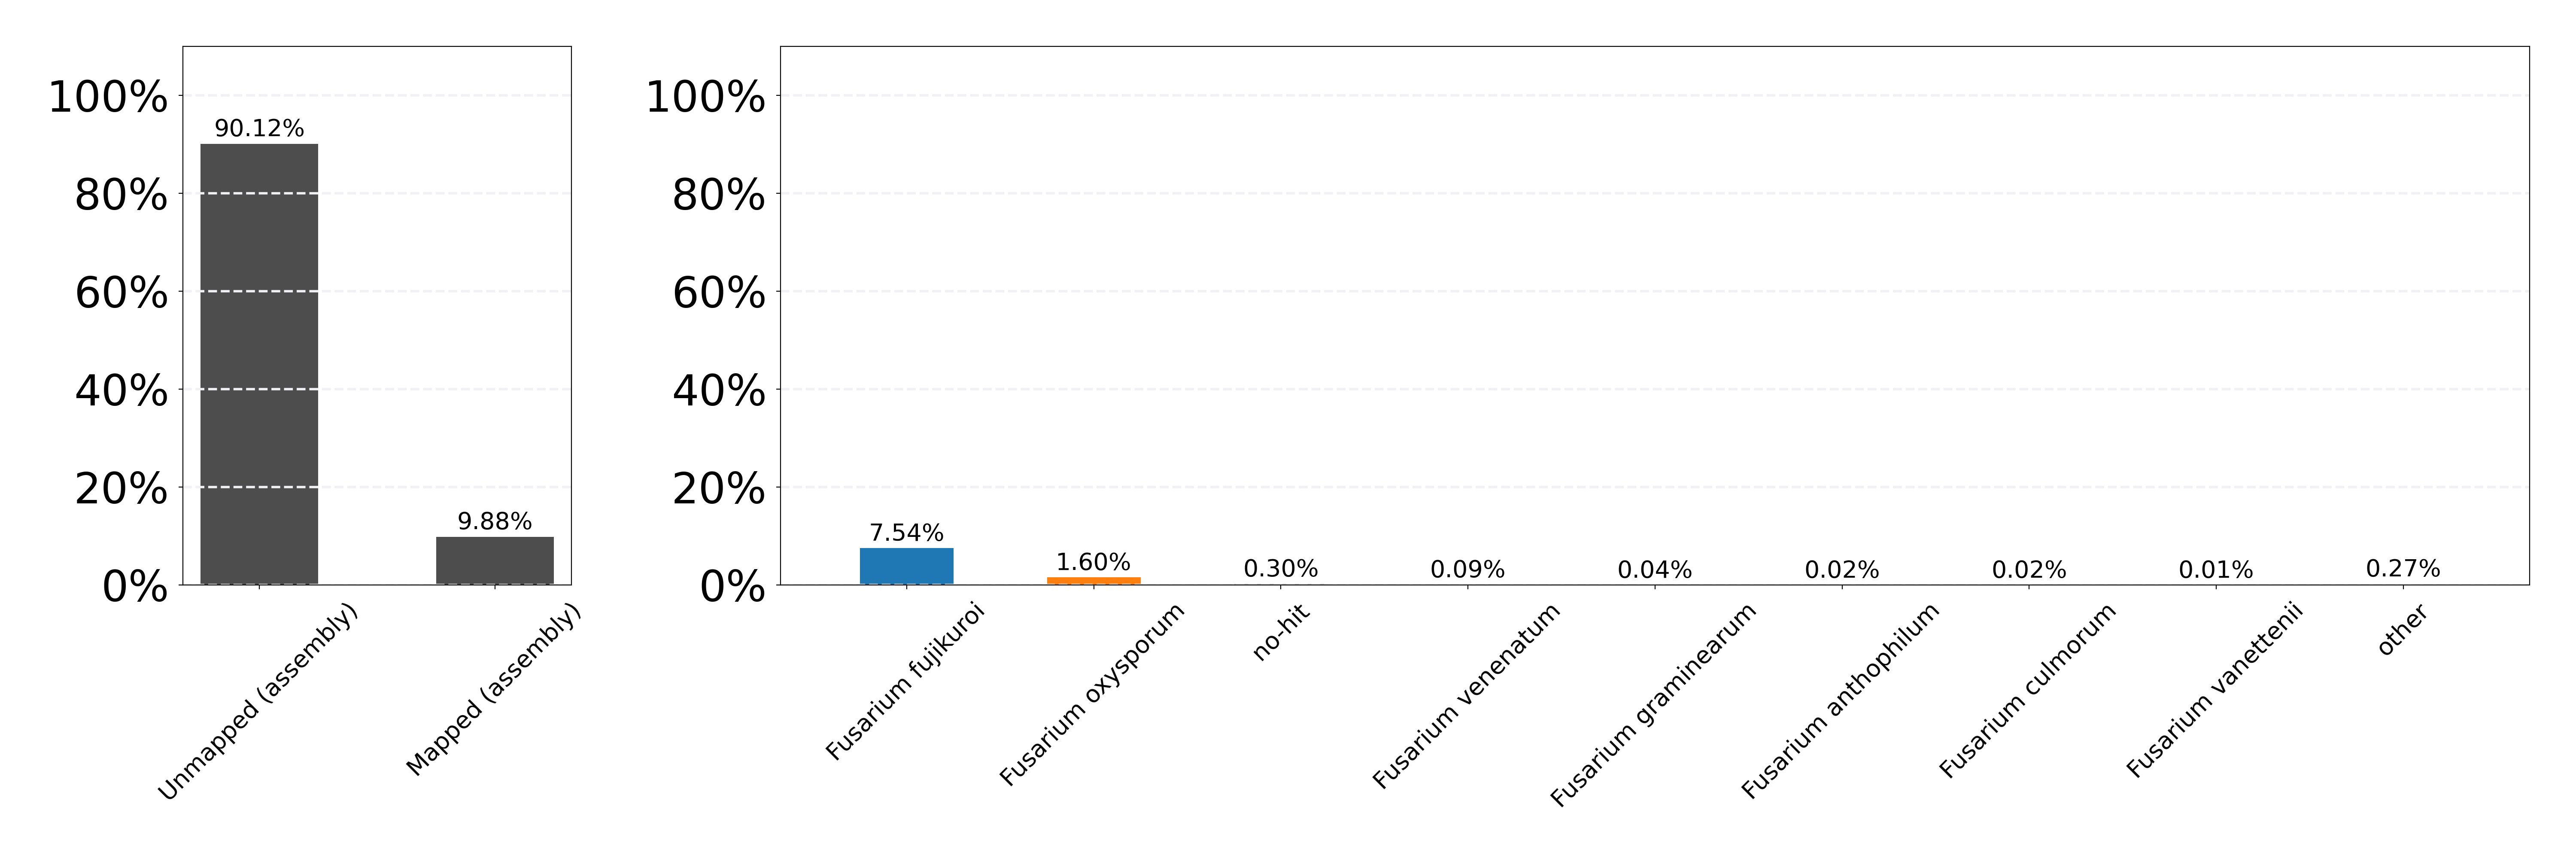
\includegraphics[width=\textwidth]{Appendices/S6_Foc1Assembly.blobtools.blobDB.json.bestsum.species.p8.span.100.blobplot.read_cov.bam0.png}
        \caption{}
        \label{fig:BlobPlot_readcov-S6}
    \end{subfigure}
    \caption[BlobTools visualisations of the S6 assembly]{\textbf{BlobTools visualisations of the S6 assembly.}
        \textbf{\subref{fig:BlobPlot-S6}) }BlobPlot of S6. Sequences in the assembly are depicted as circles, with diameter proportional to sequence length and coloured by taxonomic annotation based on BLASTN (v2.9.0+) of NCBI nt database.
        \textbf{\subref{fig:BlobPlot_readcov-S6})} Read coverage plot of the S6 assembly. Mapped reads are shown by taxonomic group at the rank of species.}
        \label{fig:S6:BlobTools}
\end{figure}



Following BlobTools (v1.1.1) analysis, contaminated contigs (assigned to species other than \textit{Fusarium}) were removed. The  S6, S16, S32, and SY-2 contaminant-filtered genome assemblies contained 6,048, 768, 2,443, and 408 contigs, respectively (Table~\ref{tab:TNAUAssemblyStats}). Coverage of the contaminant filtered assemblies varied from 16x (S6) to 148x (S16), and percentage GC content ranged from 47.53\% (S16) to 48.85\% (S32) (Table~\ref{tab:TNAUAssemblyStats}). All genome assemblies were between 40Mb and 50Mb in length and contained 15,719 to 17,891 predicted protein coding genes. Genome completeness was assessed using \ac{busco} (v5.4.6) with the hypocreales\_odb10 dataset. SY-2, S6, S16, and S32 genome assemblies contained 99.60\%, 97.50\%, 97.40\%, and 97.40\% intact, single-copy orthologs, respectively. 

% Please add the following required packages to your document preamble:
% \usepackage{multirow}
% \usepackage{longtable}
% Note: It may be necessary to compile the document several times to get a multi-page table to line up properly
\begingroup
\setlength{\tabcolsep}{20pt} % Default value: 6pt
\renewcommand{\arraystretch}{0.9}
\setlength\LTcapwidth{\textwidth} % default: 4in (rather less than \textwidth...)
\setlength\LTleft{0pt}            % default: \parindent
\setlength\LTright{0pt}           % default: \fill
\begin{longtable}[c]{ccccc}
\caption[Summary statistics of TNAU genome assemblies.]{\textbf{Summary statistics of TNAU genome assemblies. }\textit{De novo} assemblies generated using SPAdes (version 3.14.1) with all raw reads supplied by Tamil Nadu Agricultural University. }
\label{tab:TNAUAssemblyStats}\\
\hline
\multirow{\textbf{\begin{tabular}[c]{@{}l@{}}Assembly\\Statistic\end{tabular}}} & \multicolumn{4}{c}{\textbf{TNAU Isolate Assembly}} \\ \cline{2-5} 
                    & \textbf{SY-2}    & \textbf{S6} & \textbf{S16} & \textbf{S32} \\ \hline
\endfirsthead
%
\multicolumn{5}{c}%
{{\bfseries Table \thetable\ continued from previous page}} \\
\endhead
%
Number of contigs   & 441      &                & 768       & 2443        \\
Largest contig (Mb) & 0.87     &                & 0.88      & 0.77        \\
Total length (Mb)   & 44.35    &                & 44.86     & 40.92       \\
GC (\%)             & 47.97    &                & 47.53     & 48.85       \\
N50 (bp)            & 221769   &                & 234991    & 78523       \\
L50                 & 57       &                & 60        & 109         \\
Mapped Reads (\%)   & 99.6     &                & 99.53     &             \\
Mean Coverage       & 73x      &                & 148x      &             \\ 
BUSCO (\%)          & 99.6     &                & 97.4      & 97.4        \\\hline  


\end{longtable}
\endgroup

\subsubsection{Contamination in the S6 and S32 raw read data}
\label{sec:BlobToolsOfS6S32-allreads}

Since a high proportion of the genomic reads from isolates S6 and S32 originated from the bacterium \textit{S. maltophilia}, BlobTools (v1.1.1) was used to evaluate the taxonomic partitioning of \textit{de novo} assembly. These genome assemblies generated from both unfiltered and unmapped genomic raw reads contained 100,147 and 1,048 contigs, recorded  97.70\% and 97.70\% \ac{busco} intact single-copy orthologs, were 97.64 Mb and 49.62 Mb in length and had a GC content of 46.75\% and 49.80\% for S6 and S32, respectively. The S6 genome assembly generated using all raw reads was much larger than is typical for a \ac{Fo} assembly and was highly fragmented. Both genome assemblies contained a large number of contigs that were either assigned to no genera, or genera other than \textit{Fusarium}. For instance, 93,702 contigs from the S6 genome assembly had no hits and over 2,000 contigs were assigned to species other than \textit{Fusarium}, though 814 and 647 of the contigs were assigned to \ac{Ff} and \ac{Fo}, respectively (Appendix A\ref{fig:S6:BlobToolsAllreads}). The majority of contigs from the S32 \textit{de novo} genome assembly had the greatest sequence similarity to \textit{Fusarium} species, particularly \ac{Ff} (n=241), although 350 contigs had no-hits and 200 contigs were assigned to \textit{Stenotrophomonas} species, as was observed in the \acs{blast}N search of unmapped raw reads (Appendix A\ref{fig:S32:BlobToolsAllreads}). 

\subsection{\Acl{tef} and \acl{rbp2} reveal novel clade of \textit{Fusarium} pathogenic towards banana in Indian sampling region}
\label{sec:chap2phylogenies}

 Sequences containing the common \textit{Fusarium} barcodes, \acf{tef}  and \acf{rbp2}, were extracted from the \ac{tnau} isolates and used to infer a maximum-likelihood phylogeny. S6 falls within one of the \ac{Focub1} clades in the \acs{tef} and \ac{rbp2} phylogeny (Figure \ref{fig:TEF1aPhylo}, Appendix A\ref{fig:rbp2Phylo}). \Ac{tef} and \ac{rbp2} sequences from the S16 genome assembly sit within the same clade as the SY-2 and reference \ac{Fs} \ac{tef} and \ac{rbp2} sequences which, taken together with the raw read mapping data, suggests these isolates may be strains of \ac{Fs} pathogenic towards banana (Figure \ref{fig:TEF1aPhylo}, Appendix A\ref{fig:rbp2Phylo}). Based on the \ac{tef} and \ac{rbp2} phylogenies, S32 appears to be a sister lineage of \ac{Fs}. S32 groups with the newly described species recovered from symptomatic Cavendish banana in the Philippines, \acf{Fm}, proposed by \textcite{Nozawa2023}  (Figure \ref{fig:TEF1aPhylo}, Appendix A\ref{fig:rbp2Phylo}). 

These extracted \ac{tef} sequences were also searched against the Fusariod-ID MSLT and \ac{ncbi} BLAST databases for similar sequences. A search of the \ac{ncbi} database revealed that the \ac{tef} sequence extracted from the S16 genome assembly best scoring hits were for \ac{Fs} (Table \ref{tab:Tef1-NCBIdb}). Further, the Fusariod MSLT database best scoring hits for the \ac{tef} sequence extracted from the S16 genome assembly were for sequences from the \ac{FFSC}, in which \ac{Fs} can be found (Appendix A\ref{tab:Tef1-MLSTdb}). Searches for the S6 isolate extracted \ac{tef} sequence suggest S6 belongs to the \ac{FOSC}. There were matches for \ac{Focub} \ac{tef} sequences for the S6 \ac{tef} sequence, although these were not in the top 3 results from searches of both databases. No matches were found for the S32 extracted \ac{tef} sequences in the Fusarioid-ID MSLT database, and hits against the \ac{ncbi} GenBank database were for \ac{tef} sequences from \ac{Ff}. 

% Please add the following required packages to your document preamble:
% \usepackage{multirow}
% \usepackage{graphicx}
% \usepackage{lscape}
\begin{table}[h!]
\centering
\captionsetup{width=\linewidth} 
\caption[\Ac{tnau}\acf{tef} \acf{ncbi} and Fusariod-ID MSLT database searches.]{\textbf{Best hits of extracted \acf{tef} sequences from the \acf{tnau} isolate \textit{de novo} assemblies using \ac{ncbi} web-BLASTN.}}
\label{tab:Tef1-NCBIdb}
\resizebox{\columnwidth}{!}{%
\begin{tabular}{cccc}
\multicolumn{1}{l}{\multirow{2}{*}{\textbf{TNAU Isolate Assembly}}} & \multicolumn{3}{c}{\textbf{NCBI database}}                                        \\ \cline{2-4} 
\multicolumn{1}{l}{}                                       & Hit 1                    & Hit 2                    & Hit 3                       \\ \hline
\textbf{S6}                            & \textit{F. o.} isolate 170 & \textit{F. o.} f. sp. \textit{koae} & \textit{F. o.} f. sp. \textit{dianthi} \\
\textbf{S16}                                               & \textit{F. sacchari} CBS:147.25   & \textit{F. sacchari} NRLL 66326  & \textit{F. globosum} CBS:428.97      \\
\textbf{S32}                             & \textit{F. fujikuroi} I1.3        & \textit{F. fujikuroi} IMI 58289   & \textit{F. fujikuroi} Augusto2 \\ 
\textbf{SY-2} & \textit{F. fujikuroi} I1.3        & \textit{F. fujikuroi} IMI 58289   & \textit{F. fujikuroi} Augusto2 \\ \hline     
\end{tabular}%
}
\end{table}

\begin{figure}[htp!]
    \centering
    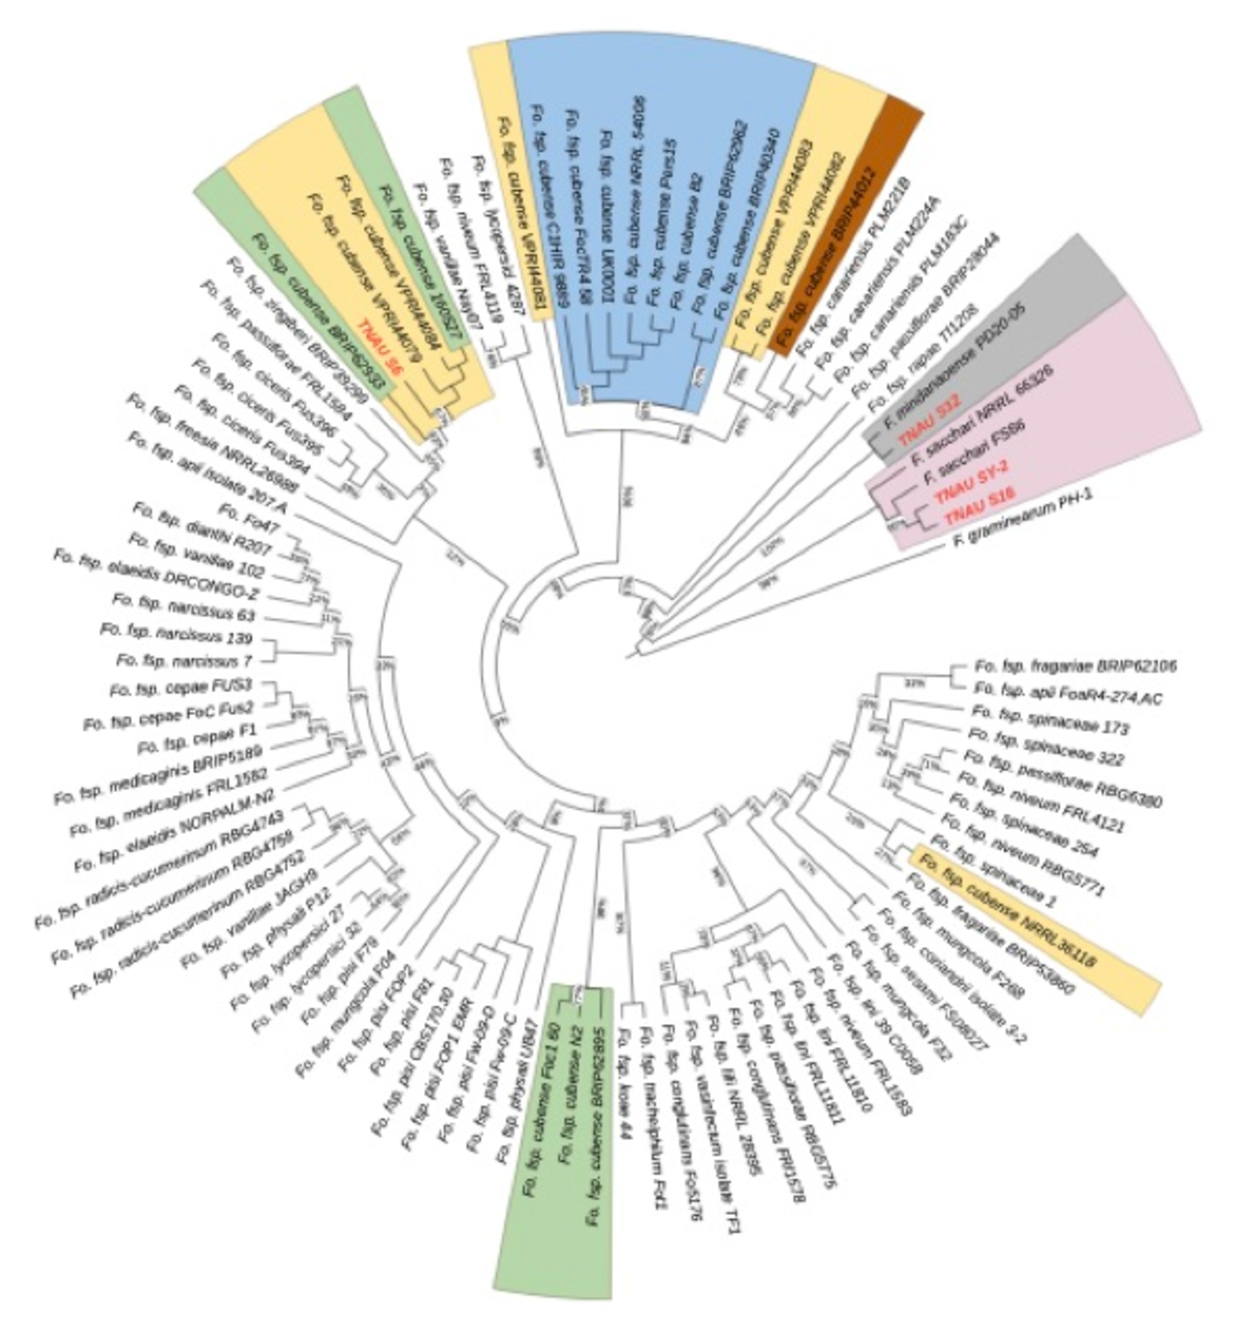
\includegraphics[width=14cm]{Figures/TEF1-aPhylo3.pdf}
    \caption[\Acl{tef} phylogeny of \acl{tnau} \textit{Fusarium} isolates.]{\textbf{\Acl{tef} phylogeny of \acl{tnau} \textit{Fusarium} isolates.} \Ac{tnau} isolates S16, S32 and SY-2 sit within the \acf{FFSC} clade. The \ac{tef} sequences from \ac{tnau} are shown in red text. The \acf{Fs} clade is shown in pink. \Acf{Focub4} \ac{tef} sequences are in blue and \acf{str4} in brown. \Acf{Focub1} \ac{tef} sequences are shown in green. The \ac{tef} sequences from \acf{Focub} genome assemblies with race not recorded are shown in yellow. Percentages represent values from 1000 bootstrap replicates. The tree is rooted through \textit{Fusarium graminearum} PH-1 \ac{tef}.}
    \label{fig:TEF1aPhylo}
\end{figure}
\bigskip

\subsection{Identification of pathogen-specific features}

\subsubsection{\textit{SIX} gene distribution suggest \ac{tnau} isolates are not \acl{Focub4}}
\label{sec:chap2SixGene}

\Acfp{sixg} are the only family of effectors currently confirmed in \ac{Fo} \parencite{Armitage2018, Czislowski2018}. \Ac{sixg} homologues (\textit{SIX1-SIX14}) were identified in the \ac{tnau} genome assemblies, alongside publicly available genome assemblies of \ac{Focub} (n=14), \ac{Fs} (n=2), \ac{Fo} \acp{fsp} (n=7), an \ac{Fo} endophyte, and a \acl{Fg} genome assembly. No \acp{sixg} were identified in the S32 genome assembly. A \textit{SIX2} homologue was identified in S16, SY-2  and  \ac{Fs} genome assemblies (Figure \ref{fig:SixTNAU}), and no other \acp{sixg} were identified. The S6 genome assembly clustered with other \ac{Focub1} isolates that have \textit{SIX1, SIX4, SIX6}, and \textit{SIX9} homologues identified, although, \textit{SIX13} is not present in the S6 genome assembly. Interestingly, no \acp{sixg} were identified in the publicly available \ac{Focub1} genome assembly, Foc1 60 \parencite{Yun2019}, which clustered with S32, as well as the \ac{Fo} endophyte and \textit{F. graminearum} genome assemblies. 

\begin{figure}[htp!]
  \centering
  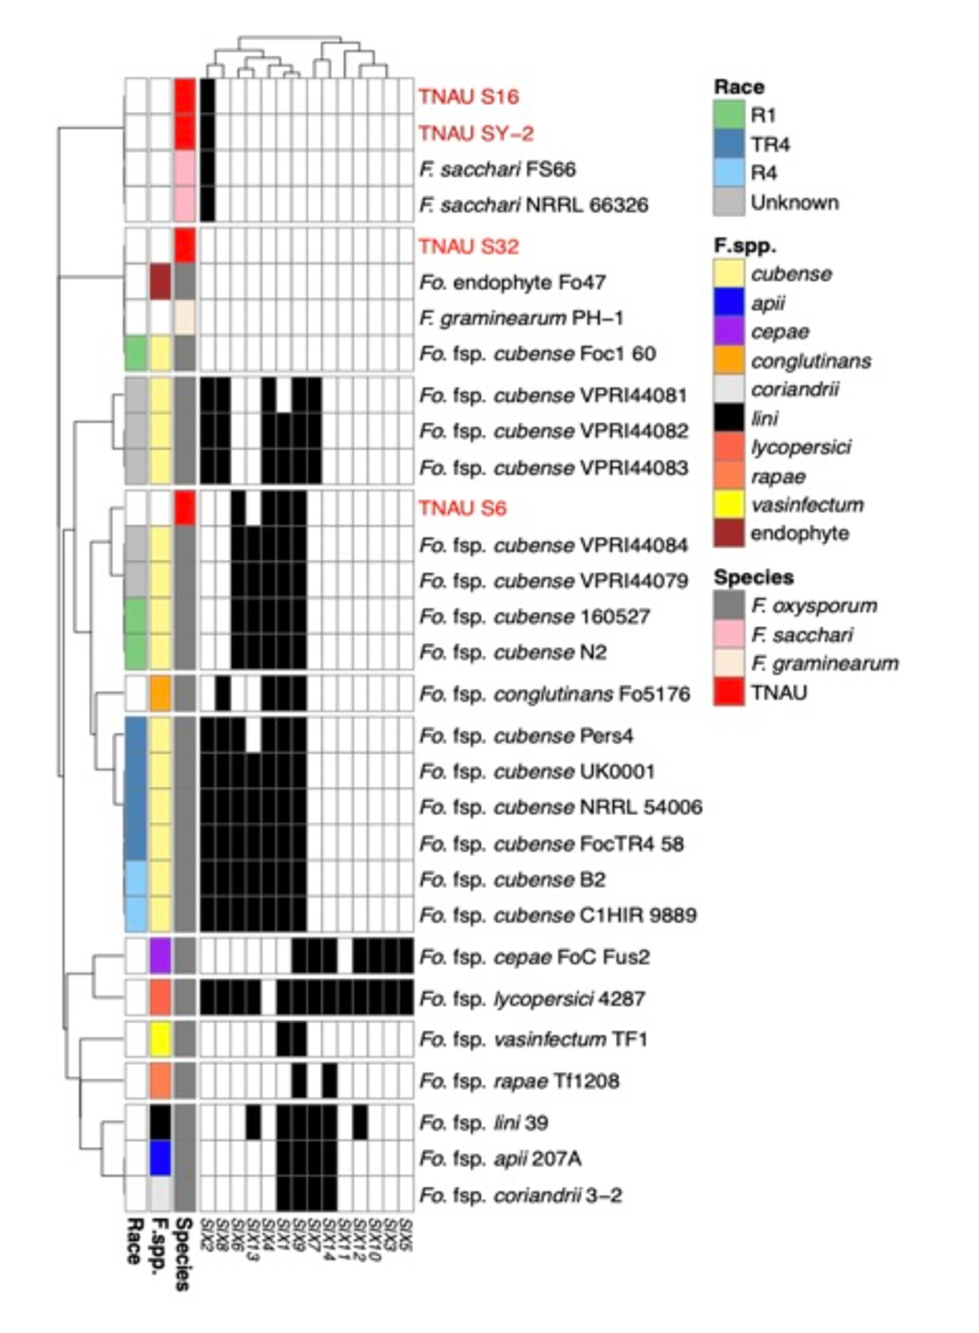
\includegraphics[width=15cm]{Figures/SIX_Heatmap.pdf}
  \caption[Binary distribution of \textit{SIX} genes across Fusarium \ac{tnau} genome assemblies]{\textbf{Binary distribution of \textit{SIX} genes across Fusarium \ac{tnau} genome assemblies}. \aclp{sixg} identified using TBLASTN (cut off 1\-e\textsuperscript{6}) using \textit{SIX} genes from \acl{Foly} as a reference. \textit{SIX4} not found in the \acl{Foly} 4287 assembly, as previously reported \parencite{Czislowski2018}}
  \label{fig:SixTNAU}
\end{figure}

As homologues of \textit{SIX1, SIX2, SIX4, SIX6}, and \textit{SIX9} were identified in the \ac{tnau} genome assemblies, these sequences were extracted for phylogenetic analysis.  A \textit{SIX9} homologue was identified in the S6 genome assembly, copies of which were identified in all \ac{Focub} genome assemblies (Figure \ref{fig:FusSIX9}). A further copy of \textit{SIX9} was found in each of the \ac{Focub4} genome assemblies and assemblies for VPRI44081, VPRI44082, and VPRI44083 (race not known). In the \textit{SIX1} phylogeny, the S6 \textit{SIX1} falls within the same clades as the \textit{SIX1} from \ac{Focub1} N2 and 160527 genome assemblies, and the \ac{Focub1} assemblies which have no race data available: VPRI44079, VPRI44082, VPRI44083, VPRI44084 (Figure \ref{fig:FusSIX1}), but the number of copies of \textit{SIX1} identified varies between isolate genome assembly. The same can also be observed for \textit{SIX4} and \textit{SIX6} (Figure \ref{fig:FusSIXMultiPhylo}). \textit{SIX2} was not identified in the S6 assembly or the \ac{Focub1} assemblies. However, it was identified in the S16 and SY-2, \ac{Fs} and other \ac{Focub} genome assemblies. The SY-2 and S16 \textit{SIX2} sequences fall within the \ac{Fs} clade in the \textit{SIX2} phylogeny (Figure \ref{fig:FusSIX2}).

\begin{figure}[htp!]
  \centering
  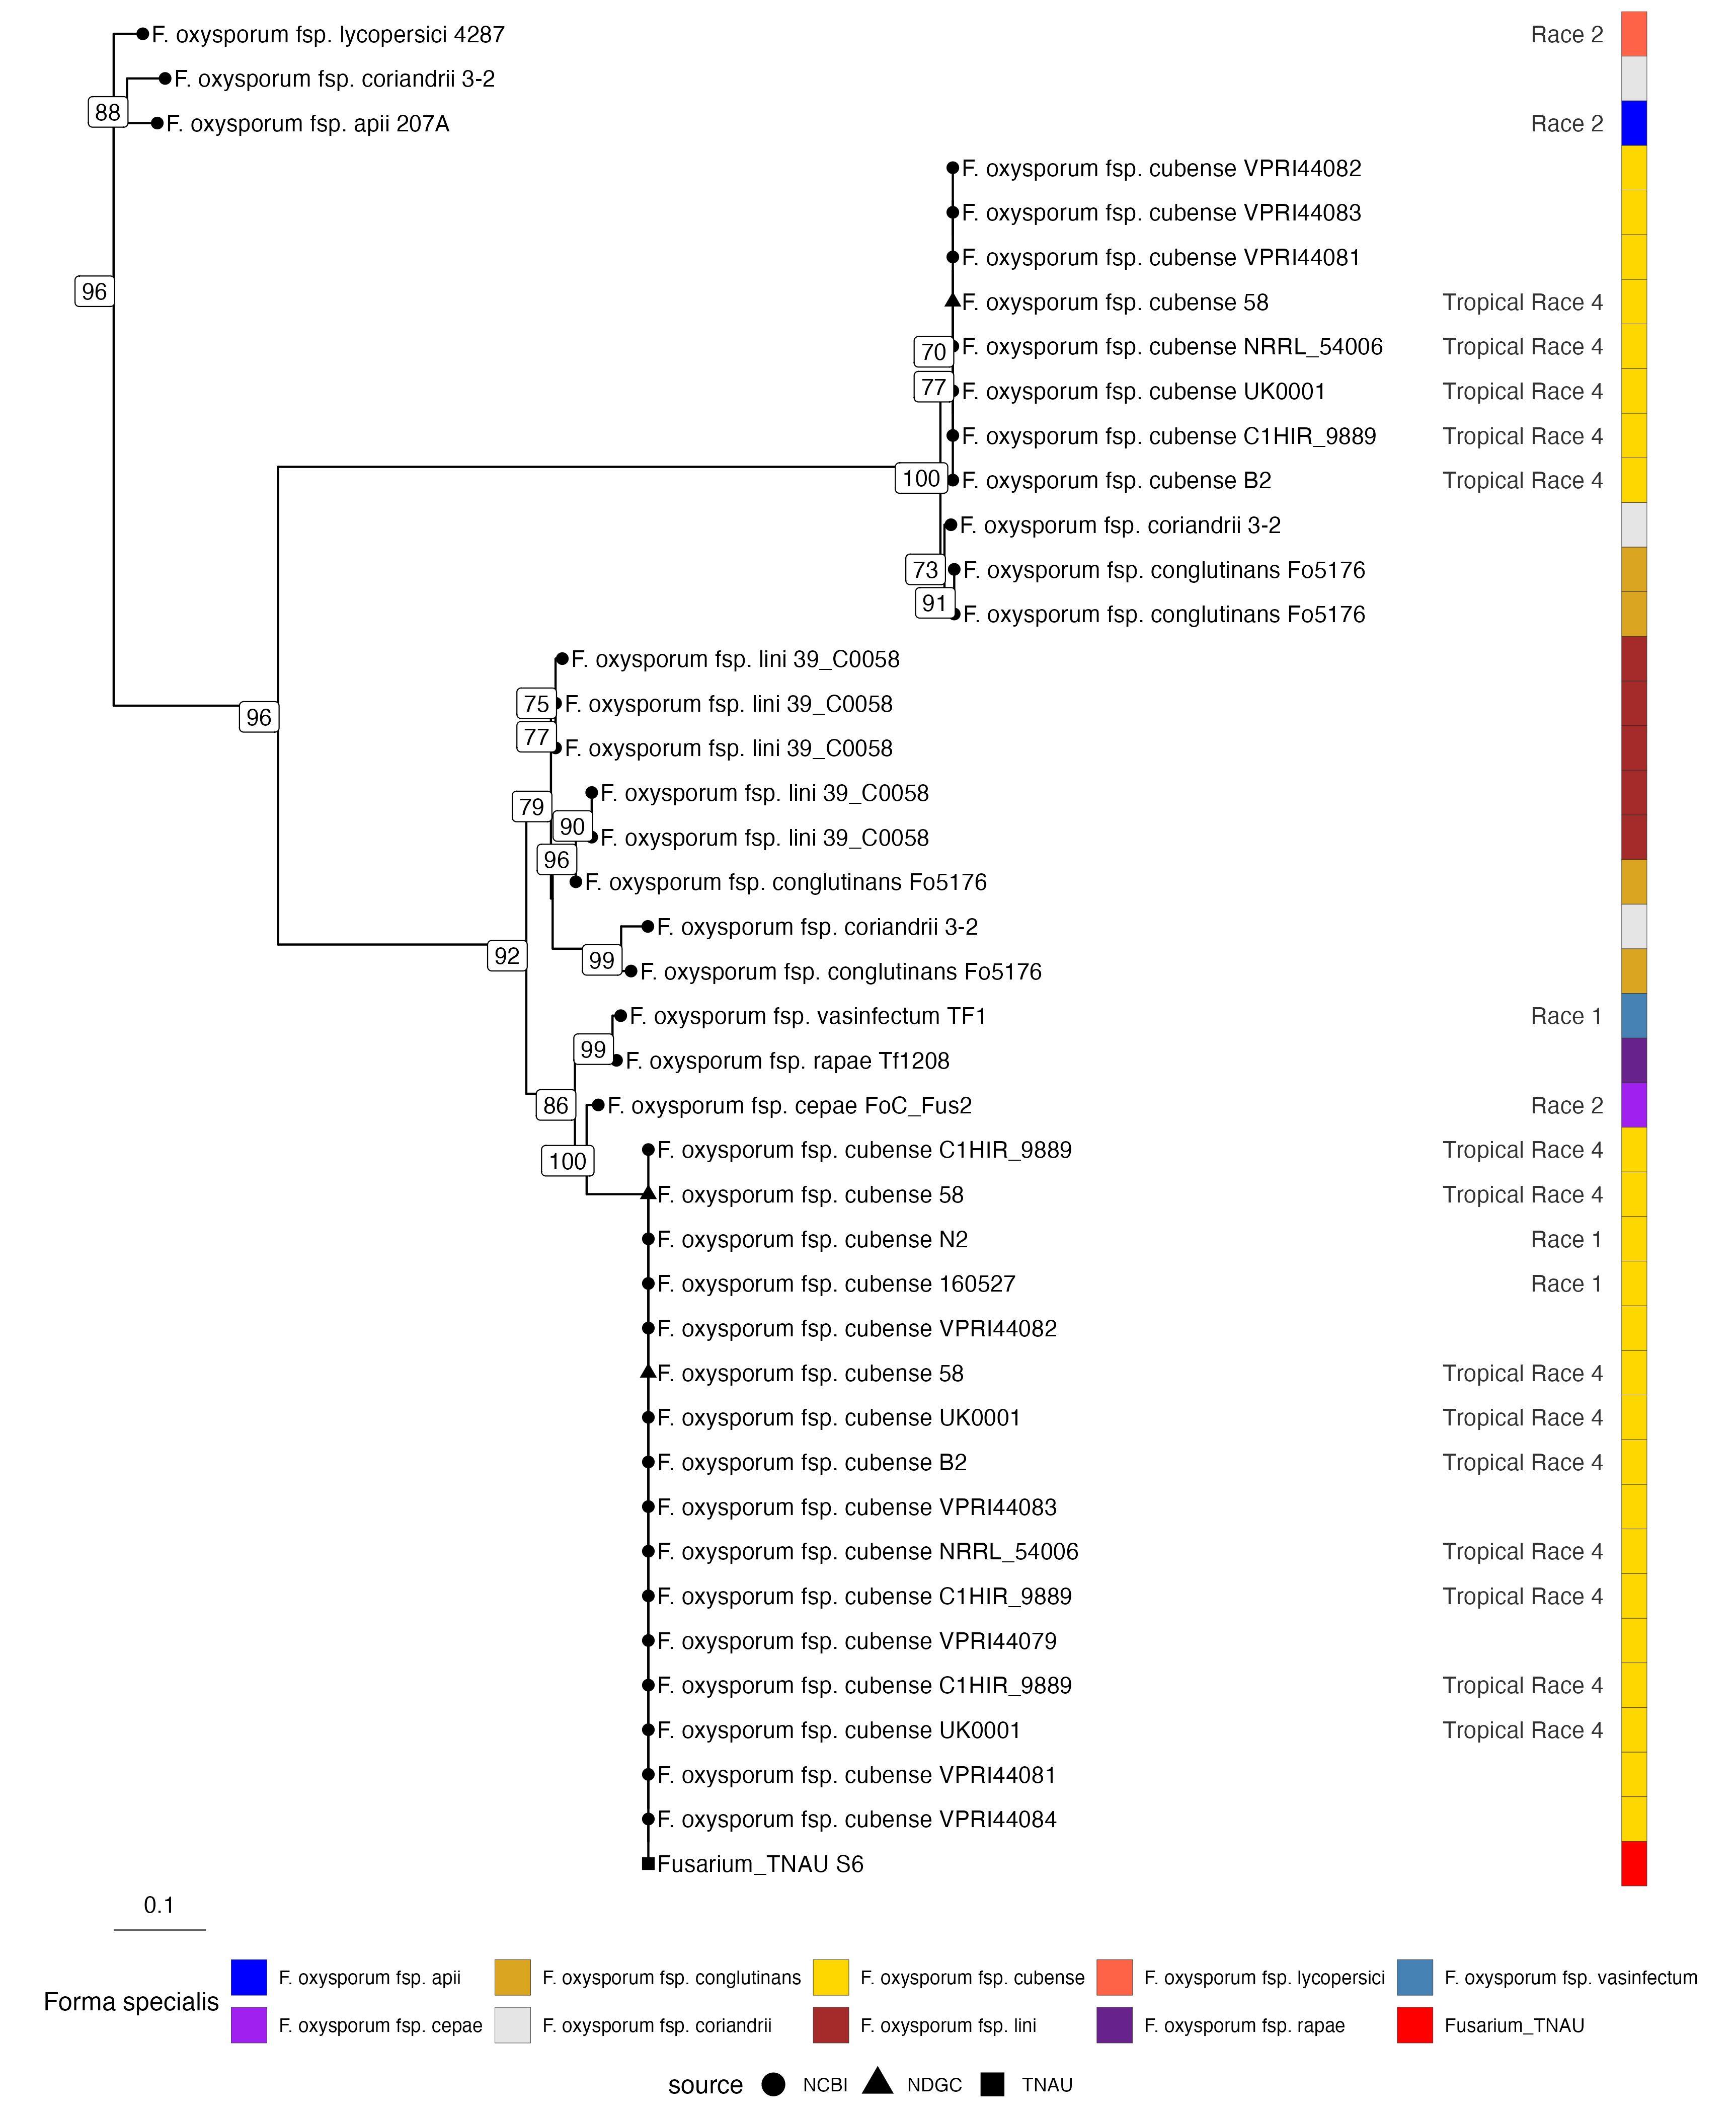
\includegraphics[width=\textwidth]{Figures/FusSIX9.phylo.png}
  \caption[Maximum likelihood phylogeny from alignment of \textit{SIX9} sequences from \textit{Fusarium} assemblies]{\textbf{Maximum likelihood phylogeny from alignment of \textit{SIX9} sequences from \textit{Fusarium} assemblies reveals \acl{Focub4} \textit{SIX9} homologue in S6}. \acl{sixg} identified by TBLASTN (cut off 1e\textsuperscript{-6}) using \textit{SIX} genes from \acl{Foly} as a reference. \textit{SIX9} sequences from \ac{tnau} are shown in red. White boxes indicate bootstrap values from 1000 bootstrap replicates. IQ-TREE2 (v2.2.0.3) best-fit model of substitution; TPM3+I. The tree is rooted through \textit{F. oxysporum f. sp. lycopersici} \textit{SIX9}.}
  \label{fig:FusSIX9}
\end{figure}

\begin{figure}[htp!]
  \centering
  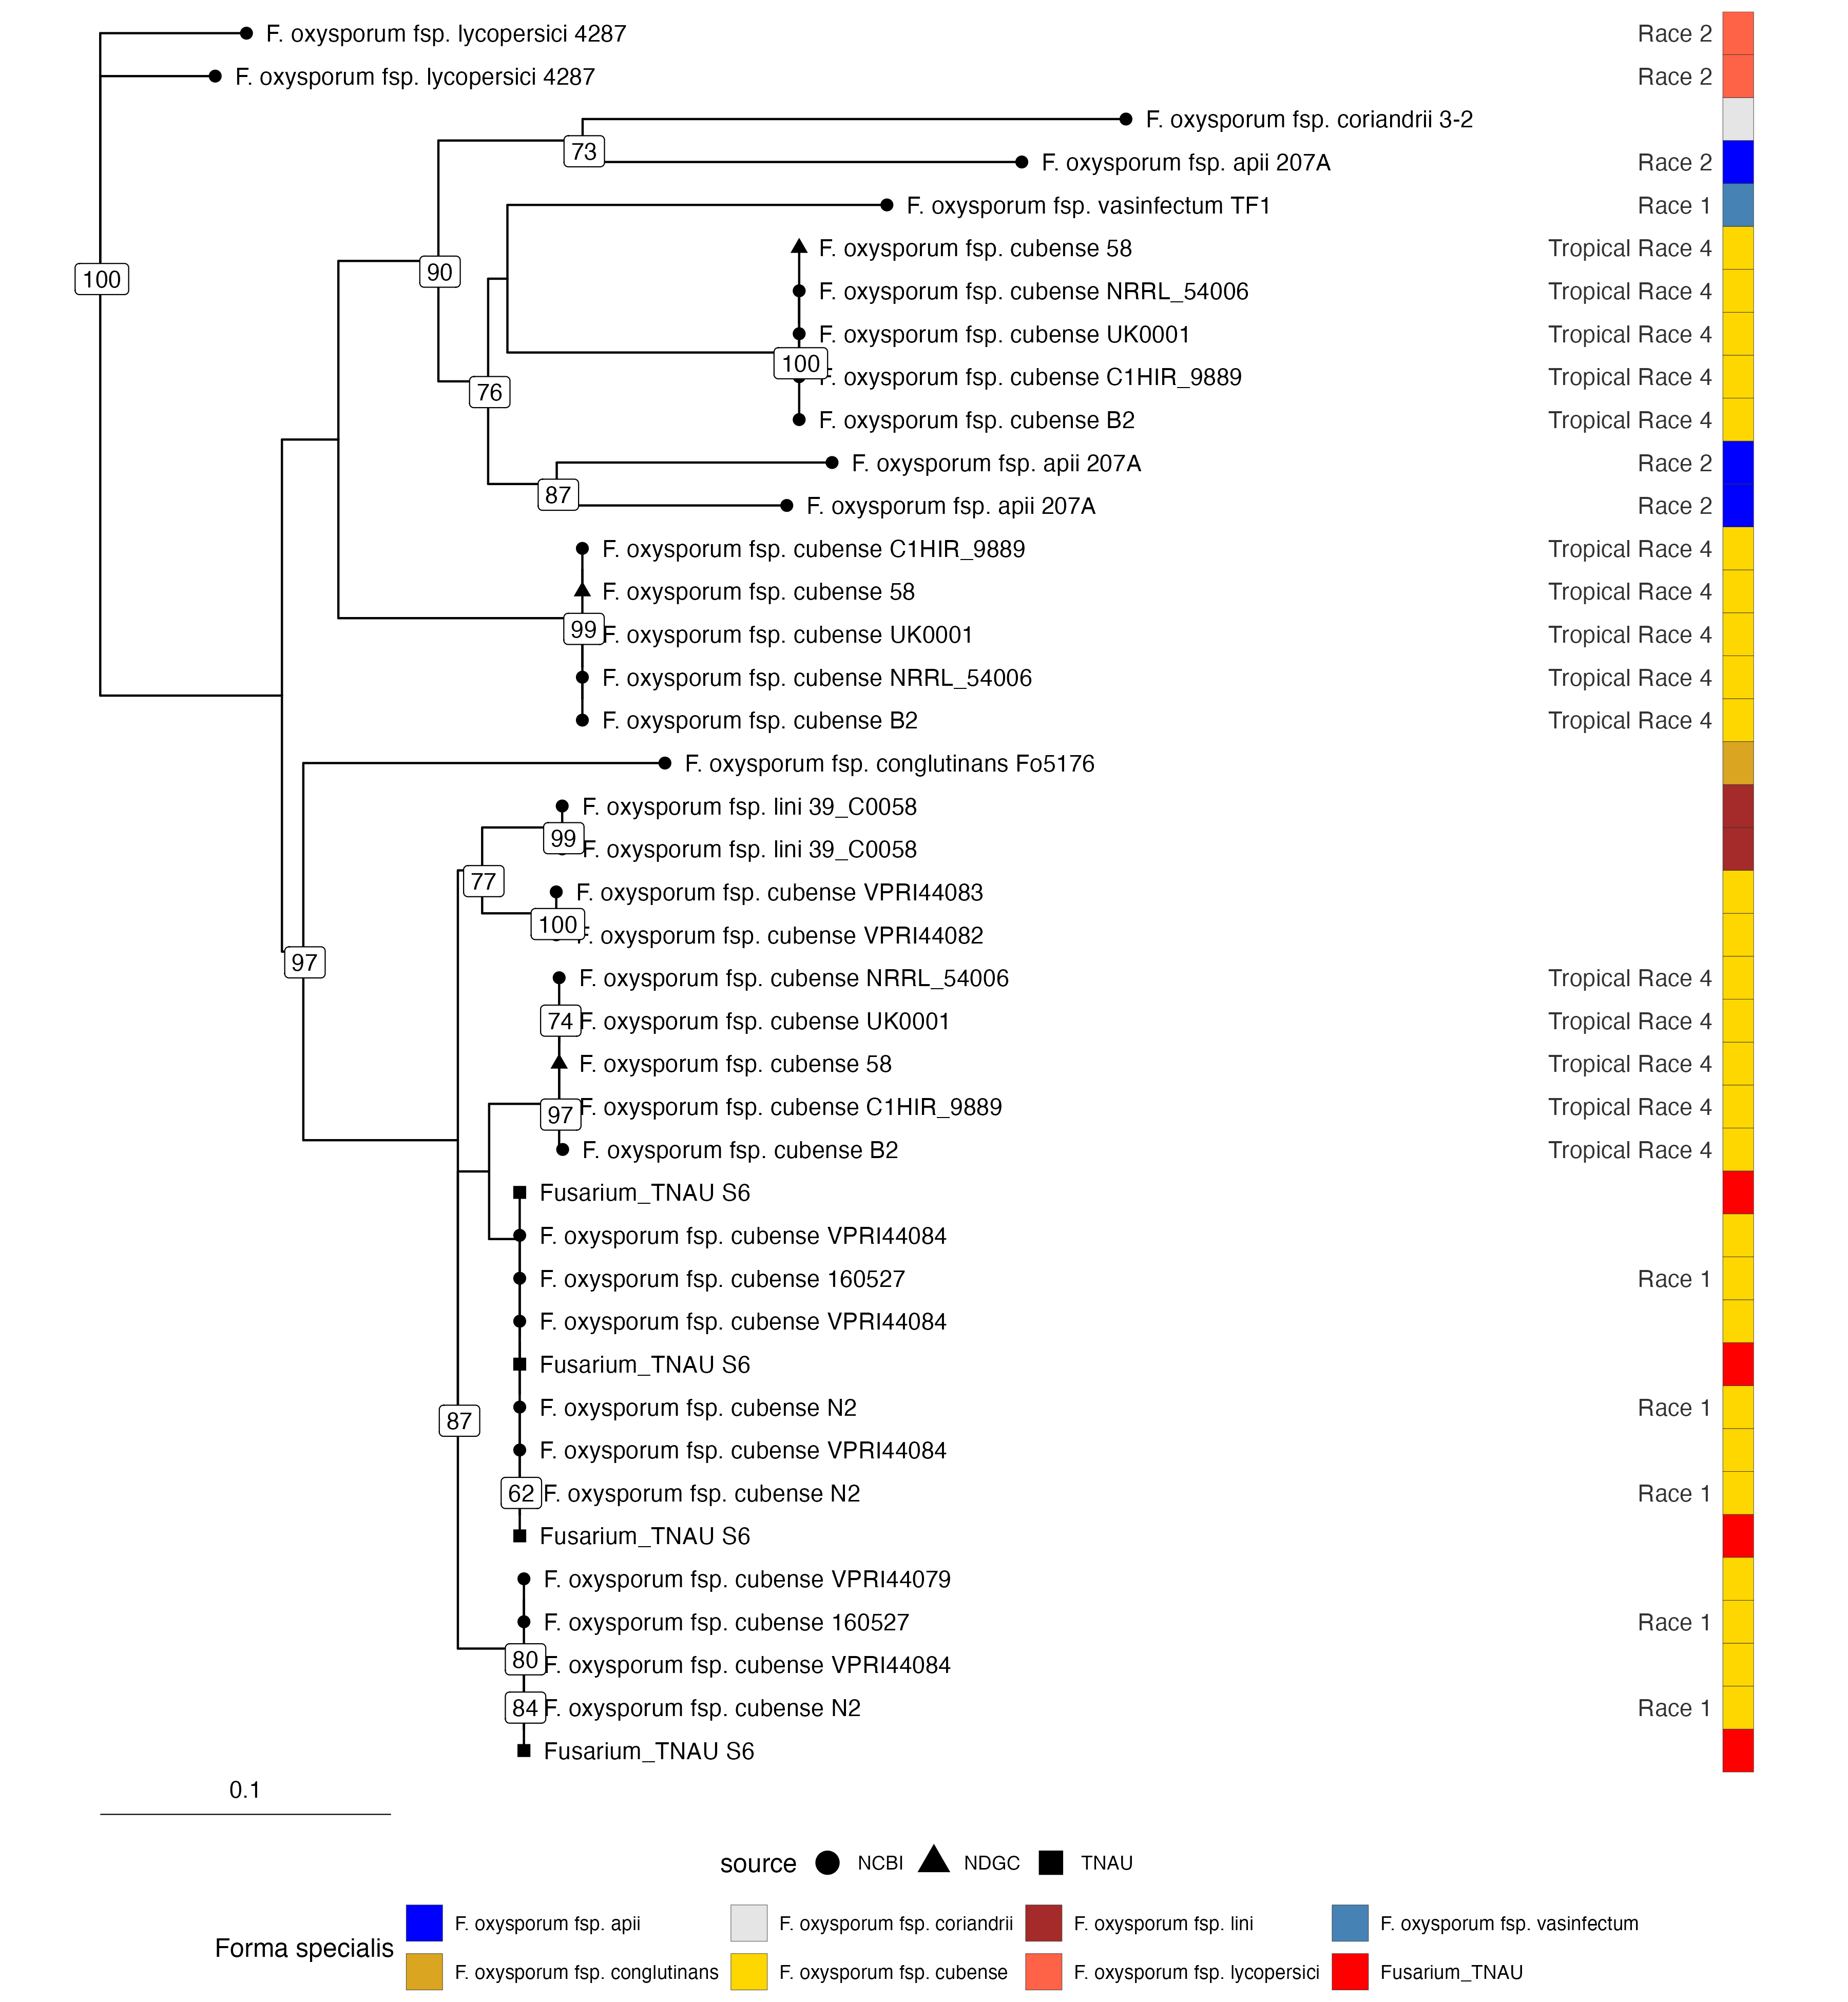
\includegraphics[width=\textwidth]{Figures/FusSIX1.phylo.png}
  \caption[Maximum likelihood phylogeny from alignment of \textit{SIX1} sequences from \textit{Fusarium} assemblies]{\textbf{Maximum likelihood phylogeny from alignment of \textit{SIX1} sequences from \textit{Fusarium} assemblies}. \textit{SIX1} identified by TBLASTN (cut off 1e\textsuperscript{-6}) using \textit{SIX} genes from \acl{Foly} as a reference. White boxes indicate bootstrap values from 1000 bootstrap replicates. IQ-TREE2 (v2.2.0.3) best-fit model of substitution; TNe+R2 The tree is rooted through \textit{F. oxysporum f. sp. lycopersici} \textit{SIX1}.}
  \label{fig:FusSIX1}
\end{figure}

\begin{figure}[hp!]
\centering
    \begin{subfigure}[]{0.9\textwidth}
        \centering
        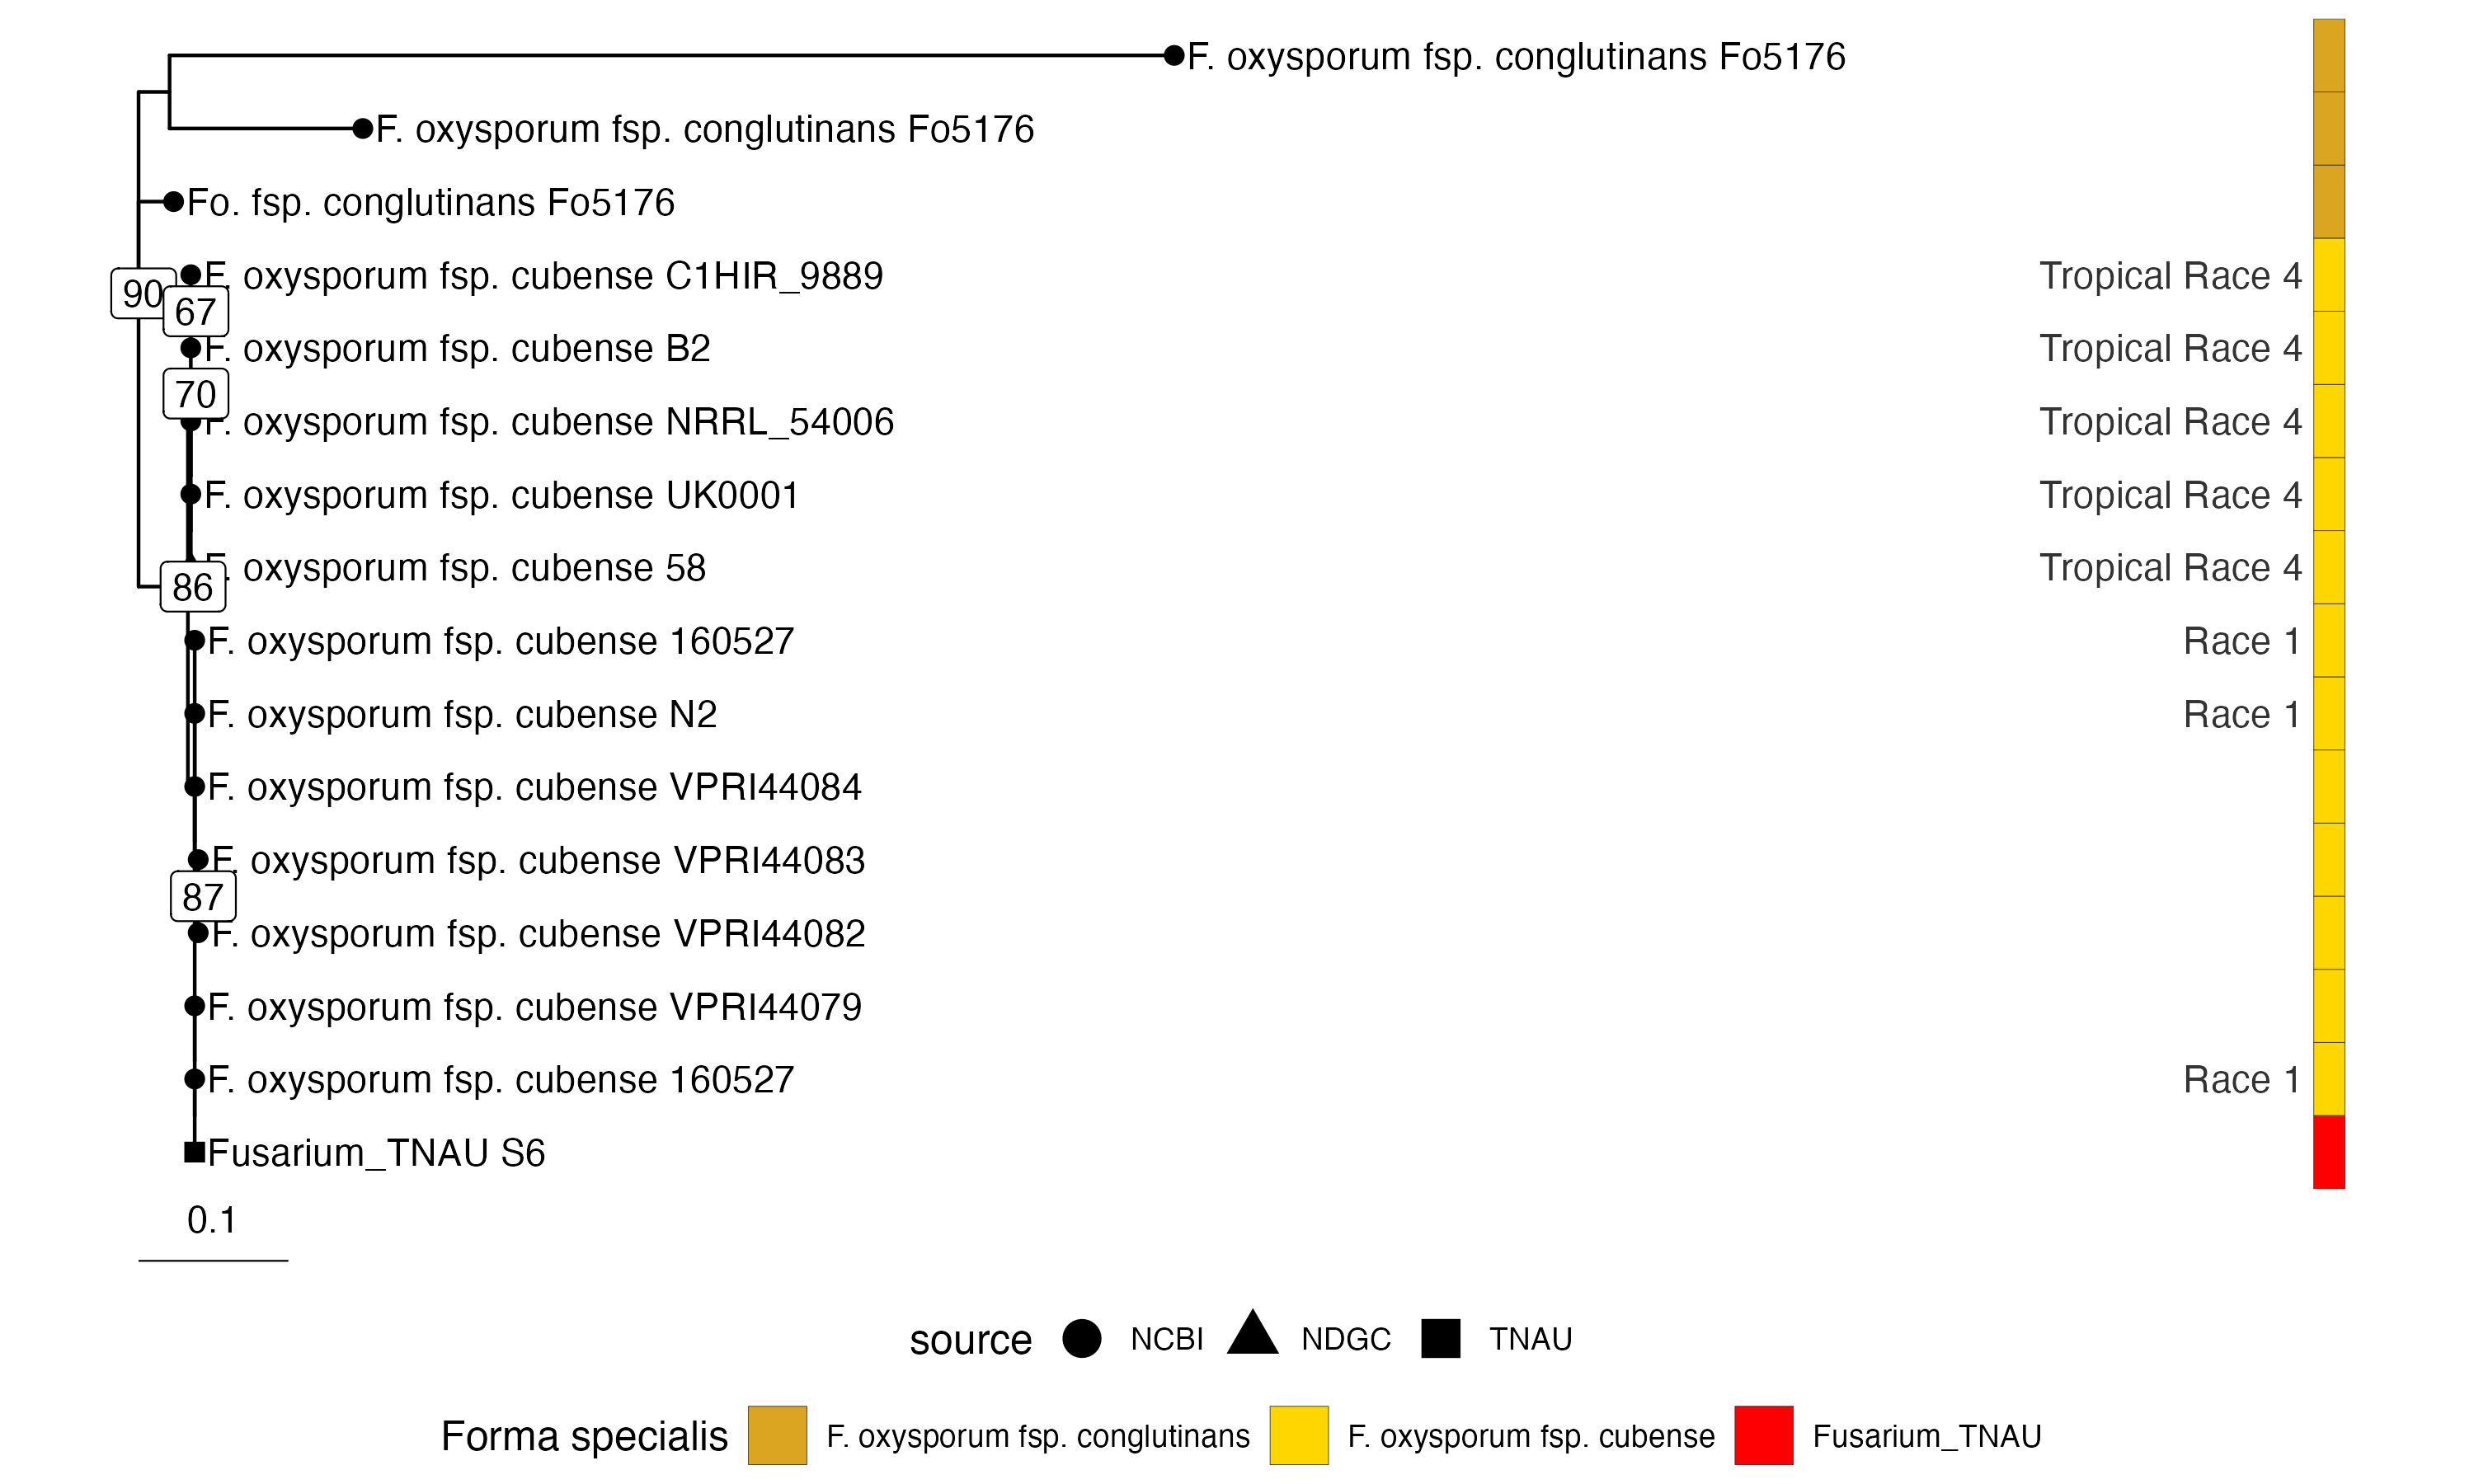
\includegraphics[width=\textwidth]{Figures/FusSIX4.phylo.png}
        \caption{}
        \label{fig:FusSIX4.phylo}
    \end{subfigure}
        \begin{subfigure}[]{0.9\textwidth}
        \centering
        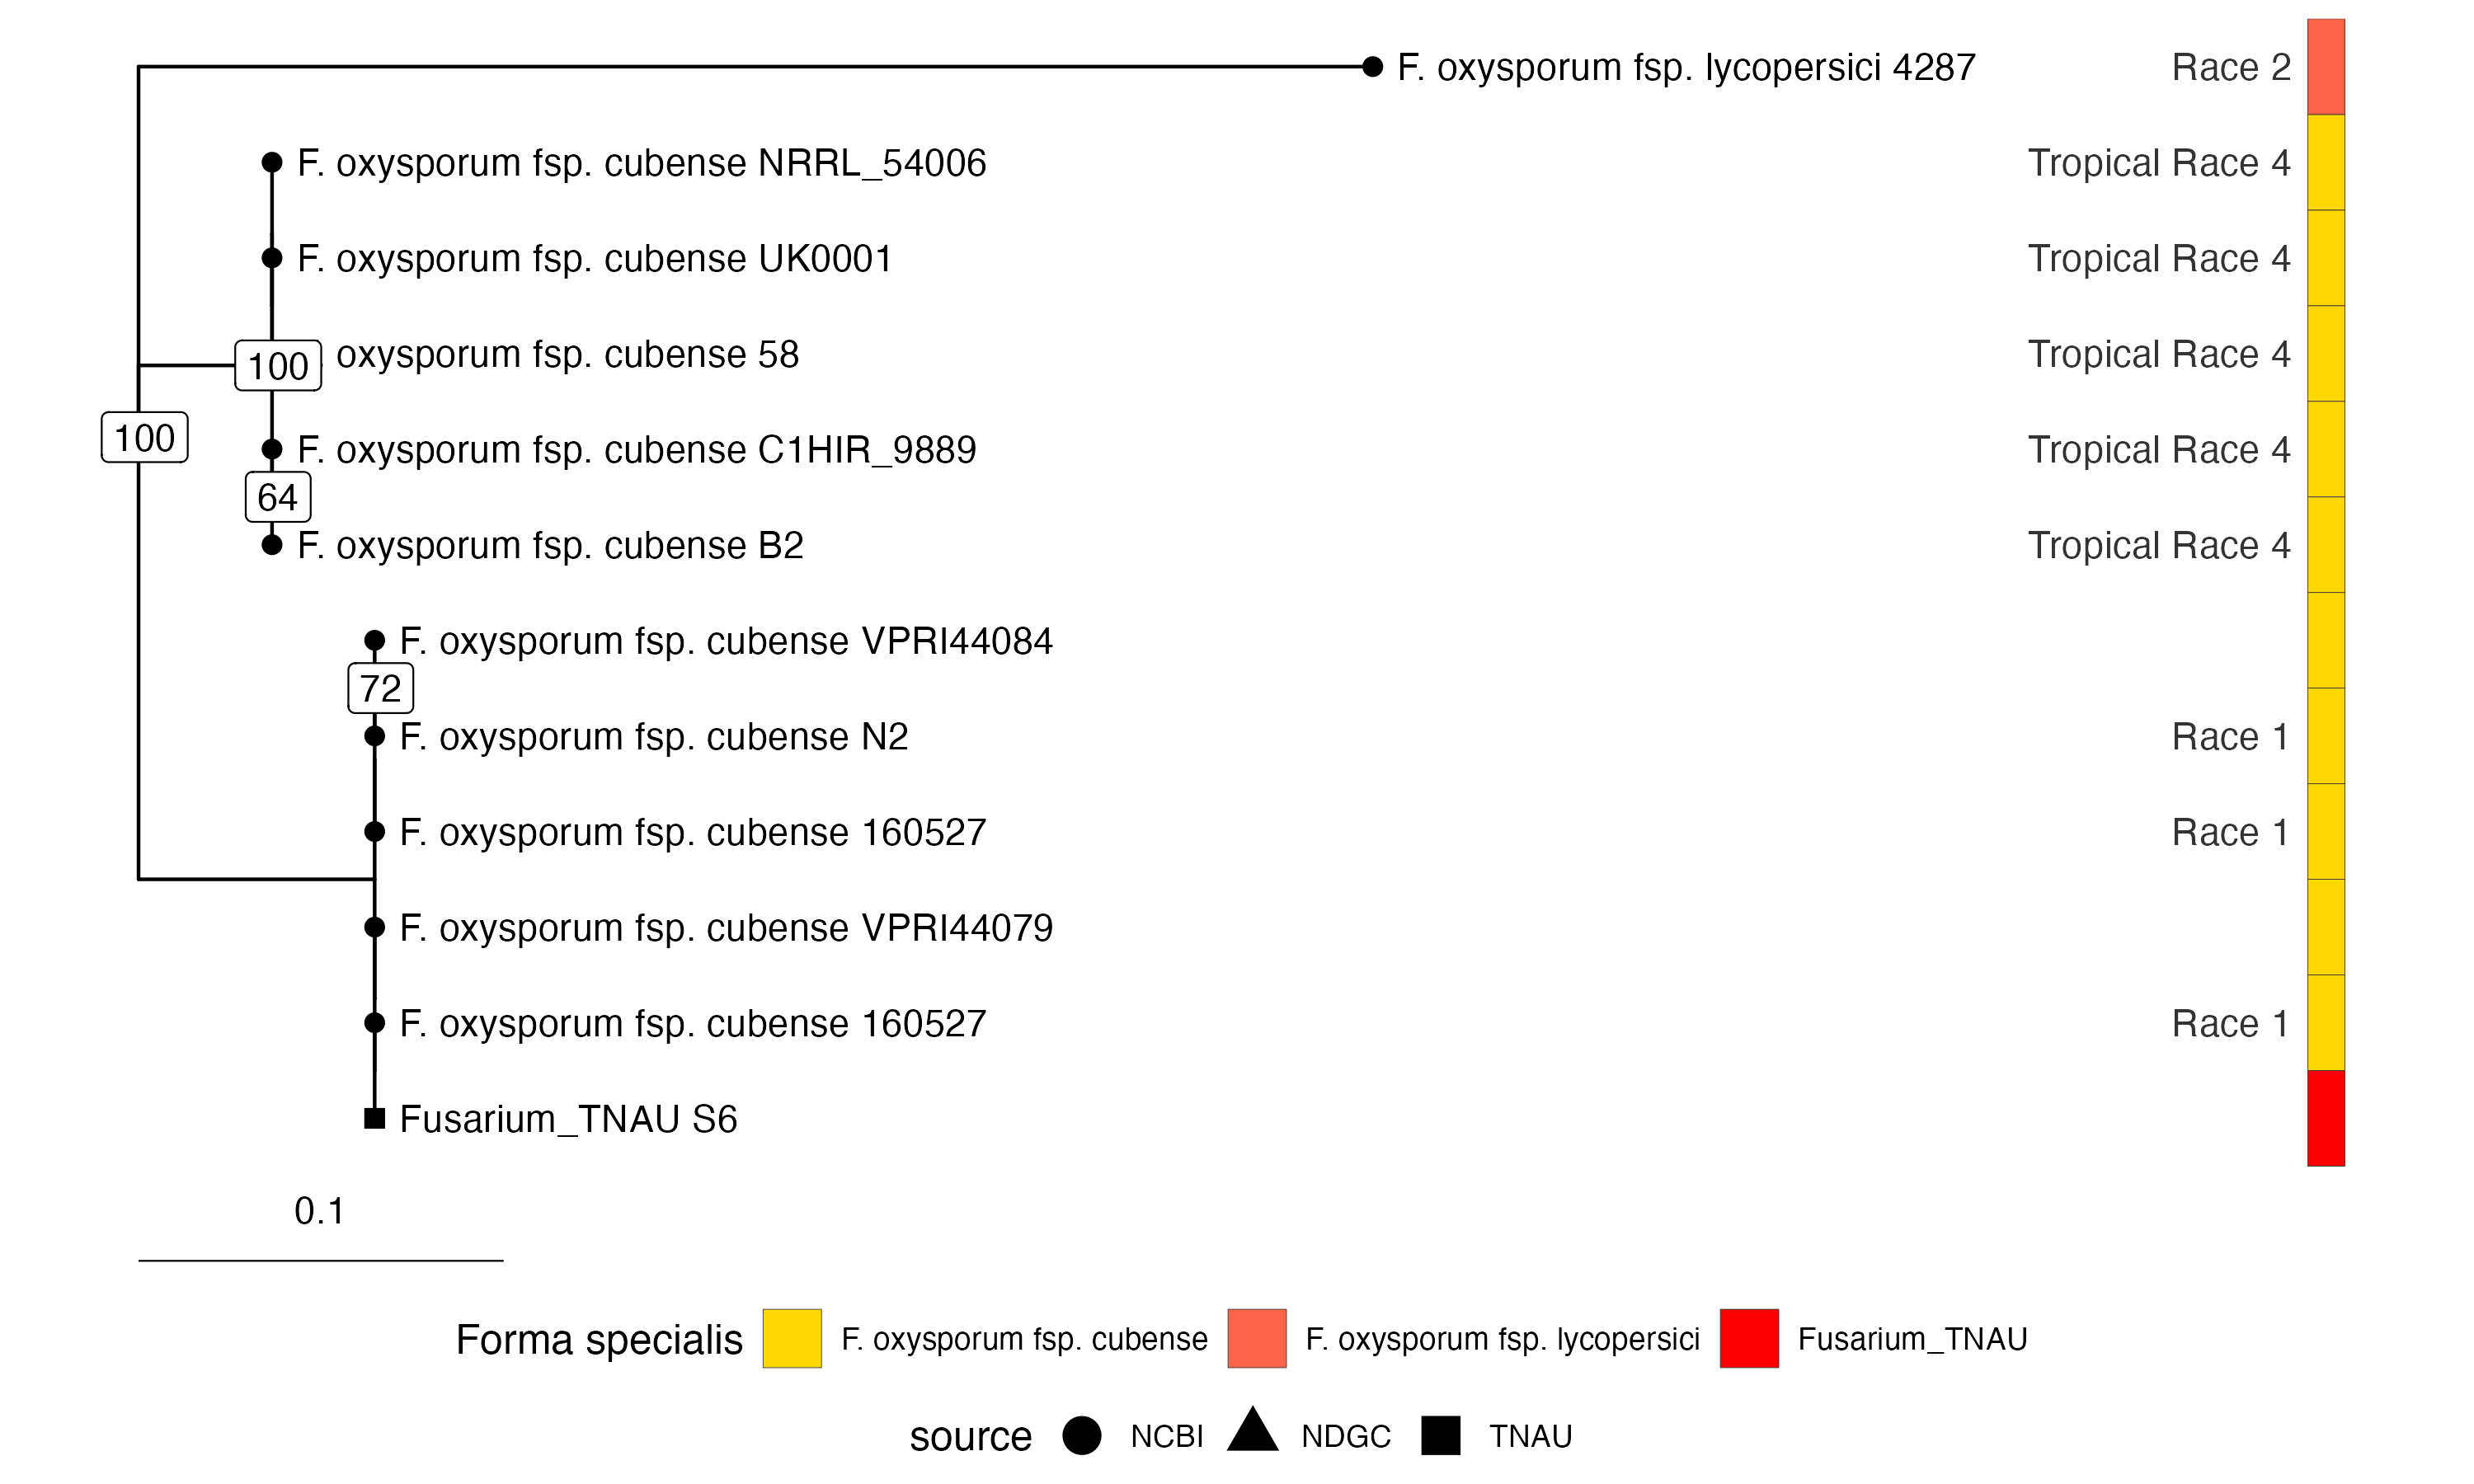
\includegraphics[width=\textwidth]{Figures/FusSIX6.phylo.png}
        \caption{}
        \label{fig:FusSIX6.phylo}
    \end{subfigure}
    \caption[Maximum likelihood phylogeny from alignment of \textit{SIX4} and \textit{SIX6} gene sequences from \textit{Fusarium} assemblies.]{\textbf{Maximum likelihood phylogeny from alignment of \textit{SIX4} and \textit{SIX6} gene sequences from \textit{Fusarium} assemblies}.
    \acl{sixg}, \textit{SIX4} and \textit{SIX6}, identified by TBLASTN (cut off 1e\textsuperscript{-6}) using \textit{SIX} genes from \acl{Foly} as a reference. White boxes indicate bootstrap values from 1000 bootstrap replicates. The IQ-TREE2 (v2.2.0.3) best-fit model of substitution for \textit{SIX4} \subref{fig:FusSIX4.phylo}); K2P. The \textit{SIX4} tree is rooted through \textit{F. oxysporum f. sp. conglutinans} \textit{SIX4}. he IQ-TREE2 (v2.2.0.3) best-fit model of substitution for \textit{SIX6} \subref{fig:FusSIX6.phylo}); K2P. The  \textit{SIX6}  tree is rooted through \textit{F. oxysporum f. sp. lycopersici} \textit{SIX6}.}
    \label{fig:FusSIXMultiPhylo}
\end{figure}

\begin{figure}[htp!]
  \centering
  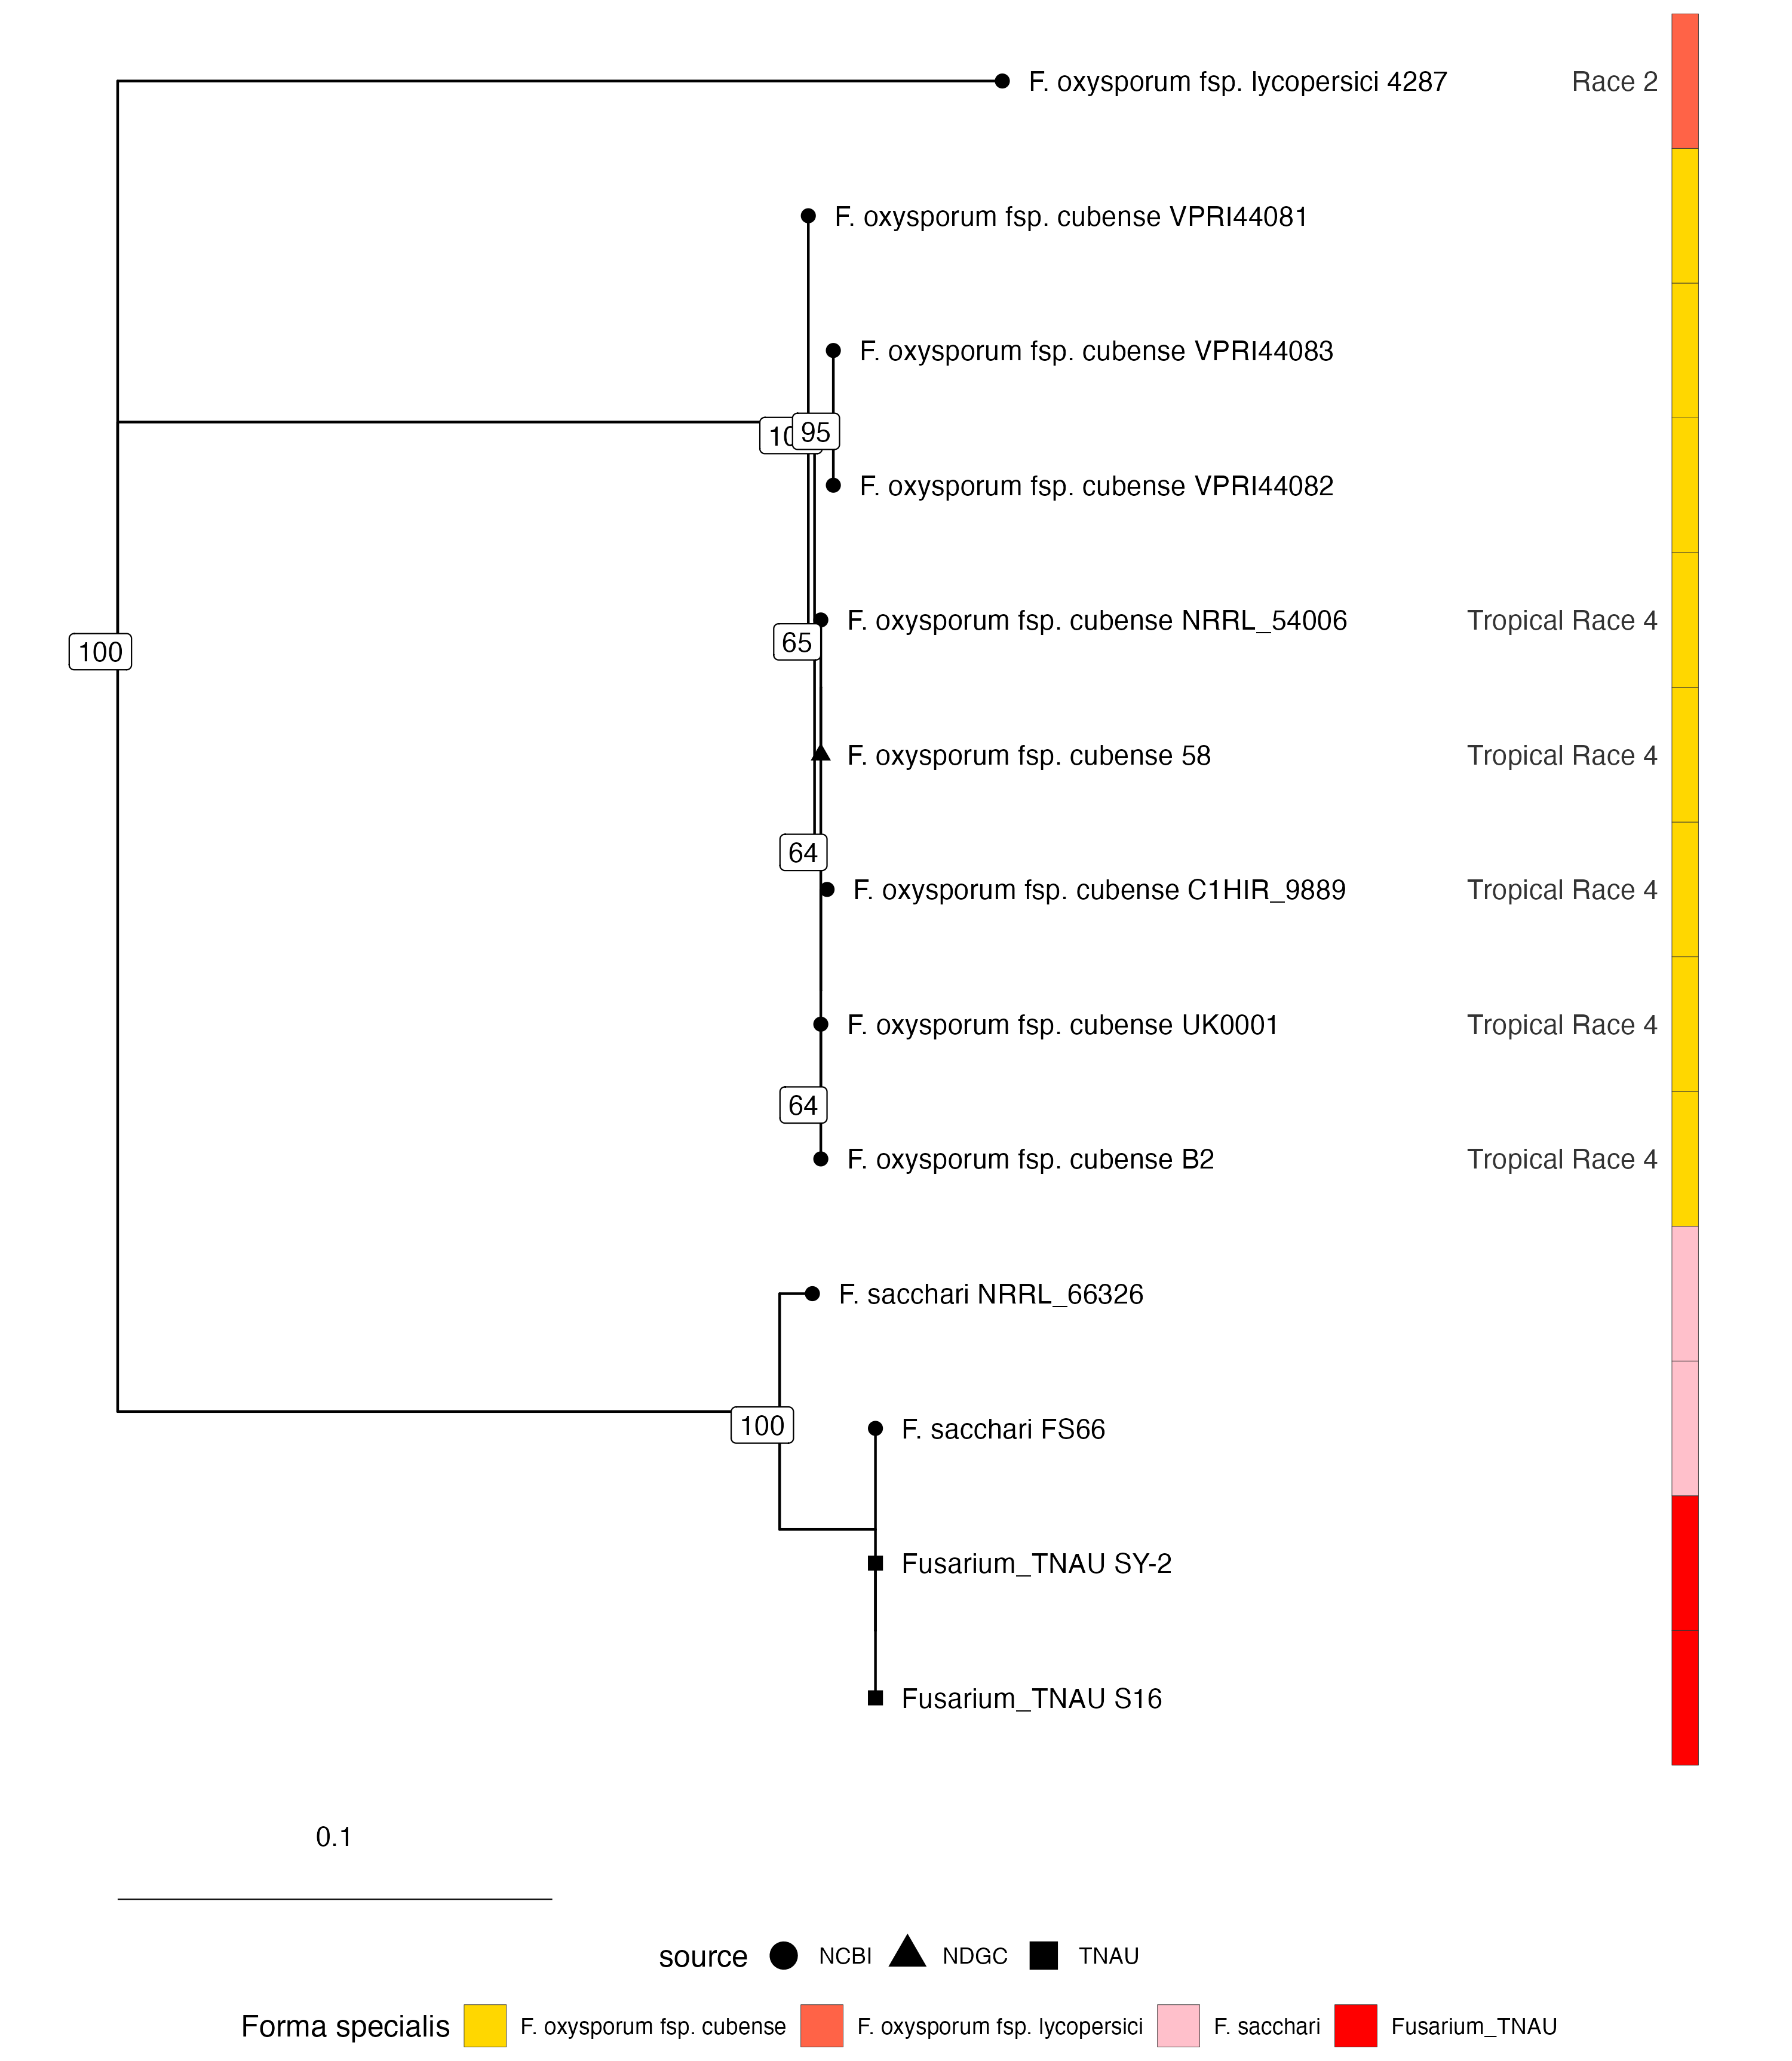
\includegraphics[width=\textwidth]{Figures/FusSIX2.phylo.png}
  \caption[Maximum likelihood phylogeny from alignment of \textit{SIX2} sequences from \textit{Fusarium} assemblies]{Maximum likelihood phylogeny from alignment of \textbf{\textit{SIX2} sequences from \textit{Fusarium} assemblies}. \textit{SIX2} genes identified by TBLASTN (cut off 1e\textsuperscript{-6}) using \textit{SIX} genes from \acl{Foly} as a reference. White boxes indicate bootstrap values from 1000 bootstrap replicates. The IQ-TREE2 (v2.2.0.3) best-fit model of substitution;  K2P. The tree is rooted through \textit{F. oxysporum} f. sp. \textit{lycopersici} \textit{SIX2}.}
  \label{fig:FusSIX2}
\end{figure}

\subsubsection{\Acl{ce} distribution in Tamil Nadu Agricultural University \textit{Fusarium} genome assemblies.}
\label{tnauCEs}

Small secreted proteins ($\geq30$aa to $\leq450$aa)  from the predicted proteomes of the \ac{tnau} genome assemblies were analysed using EffectorP (v2.0.1) to identify potential effectors. Among the genome assemblies, S6 displayed the largest \acl{ce}ome, with 333 \acp{ce}, followed by genome assembly S32 with 314 \acp{ce}, while both SY-2 and S16 had 289 \acp{ce} each. Of these candidates, 132 were conserved between all genome assemblies when clustered at 80\% identity (Figure \ref{fig:TNAUVenn}). S6 also had the largest number of unique candidates when clustering at this percentage identity threshold, totalling 138. S32 had the next largest number of unique candidates, at 68. 70 of the candidates were shared between the S16 and SY-2 genome assemblies, but not the other genome assemblies. A total of 69 candidates were shared between S16, S32, and SY-2 but not in S6, and 39 candidates were shared between S6 and S32 but were not identified in SY-2 or S16 at the  80\% identity threshold. 

\begin{figure}[h!]
  \centering
  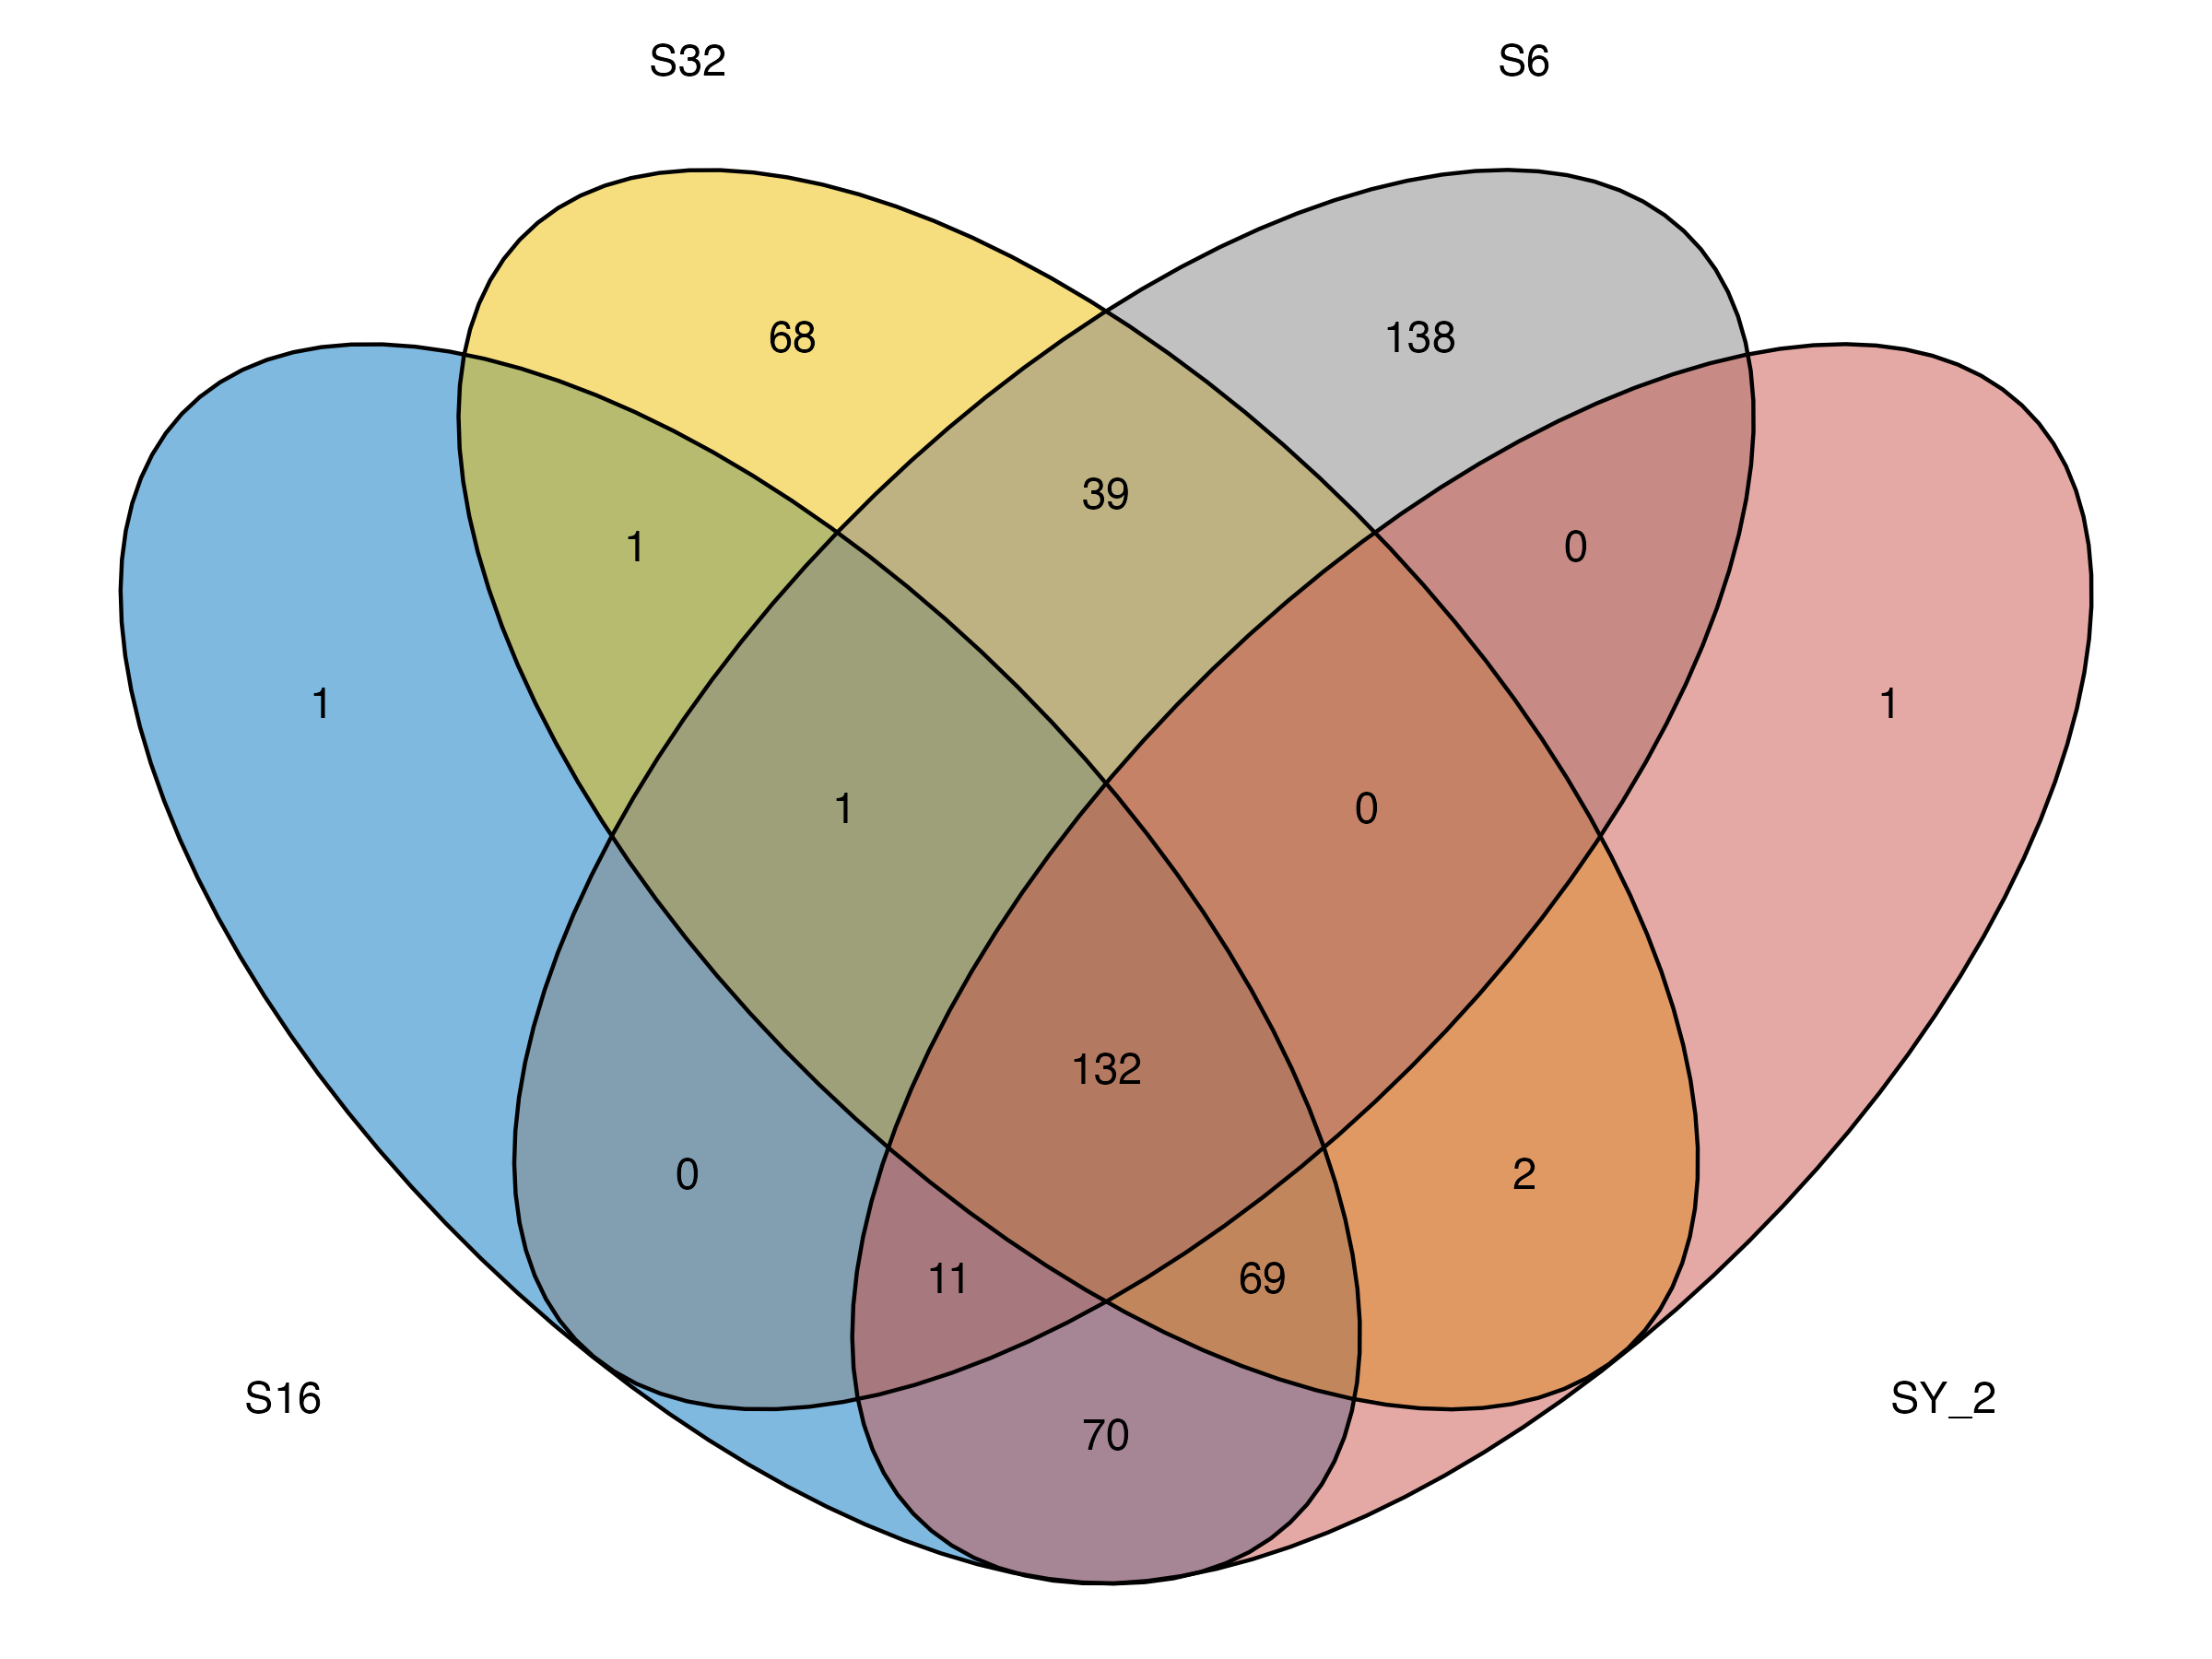
\includegraphics[width=\textwidth]{Figures/sharedCandEffsVenn.png}
  \caption[Distribution of \acp{ce} among Tamil Nadu Agricultural University \textit{Fusarium} genome assemblies.]{\textbf{Distribution of \acp{ce} among Tamil Nadu Agricultural University \textit{Fusarium} genome assemblies.} Numbers represent the total \acp{ce}. SY-2=red oval, S6=grey oval, S16=blue oval, S32=yellow oval.}
  \label{fig:TNAUVenn}
\end{figure}


%%%%%%%%%%%%%%%%%%%%%%%%%%%%%%%%%%%%%%%%%%%%%
%DISCUSSION
%%%%%%%%%%%%%%%%%%%%%%%%%%%%%%%%%%%%%%%%%%%%%
\clearpage
\section{Discussion and Conclusions}

Collaborators at \ac{tnau} investigated \ac{Focub} diversity in Tamil Nadu. They surveyed banana-growing areas, collecting samples from symptomatic banana, including the Cavendish variety, 'Grande Naine'. Of the isolates collected, SY-2, S6, S16, and S32 were chosen for further study due to their highly virulent phenotype on Cavendish banana. Collaborators report (personal communication) that \ac{PCR} analysis confirmed SY-2, S6, S16, and S32 identity as \ac{Focub4} isolates\footnote{Using \textit{SIX9} primers from \textcite{Carvalhais2019}. It is important to note that collaborators at \ac{tnau} did not show data supporting their conclusions.}. However, our study does not support their conclusions. Genomic analysis suggests that banana-pathogenic isolate S32 belongs to a clade within genus \textit{Fusarium} species that may represent an as-yet undescribed species, that S6 belongs to a clade usually associated with \ac{Focub1}, but has acquired a \ac{Focub4} phenotype. Isolates SY-2 and S16 appear to belong to \ac{Fs}, a species recently reported to be potentially pathogenic towards banana, having acquired genes from \ac{Fo} \parencite{Cui2021}. Interestingly, SY-2 and S16 are reported to display symptoms consistent with \ac{fwb} by collaborators at \ac{tnau}, whereas the \ac{Fs} isolate pathogenic towards Cavendish reported by \textcite{Cui2021} (FS66) displays foliar blight symptoms. As we have not been able to access the \ac{tnau} \textit{Fusarium} isolates, we have been unable to compare symptoms to FS66, the \ac{Fs} isolate pathogenic towards Cavendish reported by \textcite{Cui2021}. 

Initially, the raw read data supplied by collaborators at \ac{tnau} were aligned to high-quality \ac{Focub4} (\href{https://www.ncbi.nlm.nih.gov/datasets/genome/GCA_007994515.1/}{GCA\_007994515.1}) and \ac{Focub1} (\href{https://www.ncbi.nlm.nih.gov/datasets/genome/GCA_005930515.1/}{GCA\_005930515.1})  assemblies for a reference-guided assembly approach. However, alignment rates and web BLASTN searches of the unmapped reads against the nr/nt database contradicted TNAU's initial classifications, and revealed bacterial contamination in the S6 and S32 datasets. Later supported by BlobTools (v1.1.1) analysis of \textit{de novo} assembly constructed using all raw reads (See section: \ref{sec:BlobToolsOfS6S32-allreads}). Consequently, raw reads were  mapped to assemblies for which a large number of highly similar ($ \geq90\% $ identity) BLASTN hits were identified. Genome assemblies for SY-2, S16, and S32 showed closer alignment to the \textit{F. sacchari} reference compared to the \ac{Focub} references, and S6 and S32 contained contamination from \textit{S. maltophilia}. 

As these results suggested that SY-2, S16, and S32 are not \ac{Focub4} isolates, it was no longer clear which species should be used as a reference for a reference-guided assembly. Further, the \ac{tnau} isolates displayed a highly virulent phenotype and a reference-guided assembly could lose any large-scale rearrangements in the genome which may contribute to this phenotype. However, contamination in the S6 and S32 data meant that a \textit{de novo} genome assembly for these isolates was likely to result in misassembled contigs that are chimeric (part target species, part non-target species). These contigs can be challenging to identify and may result in contigs that should remain in the assembly being filtered out, and contigs that do not belong to the target species being kept in the assembly, even when using BlobTools (v1.1.1.) to separate target and non-target contigs \parencite{Cornet2022}, so must be removed from the raw read data. 

Consequently, genomes for SY-2 and S16 were assembled \textit{de novo} and S6 and S32 were assembled \textit{de novo} using only the reads that mapped to reference genomes with the highest mapping value. For S6, therefore, a \textit{de novo} genome assembly was generated using the raw reads which mapped to \ac{Focub1} 160527 (\href{https://www.ncbi.nlm.nih.gov/datasets/genome/GCA_005930515.1/}{GCA\_005930515.1}) reference and for S32 a \textit{de novo} assembly was generated using the raw reads which mapped to the \ac{Fs} FS66 (\href{https://www.ncbi.nlm.nih.gov/datasets/genome/GCA_017165645.1/}{GCA\_017165645.1}) reference. BlobTools (v1.1.1) was used to confirm that the levels of contamination in the assemblies had been reduced, pinpoint any potential contaminant contigs to remove, and support isolate classification. Predicted protein coding genes, percentage GC content, size, and \ac{busco} scores for the contaminant filtered assemblies were comparable to other \textit{Fusarium} short-read assemblies (see: \textcite{DitaHerai2013, Chiara2015, Srivastava2018}).

As the identity of \ac{tnau} isolates was uncertain, we queried the genetic markers \acf{tef} and \acf{rbp2} extracted from the assemblies against Fusariod-ID MSLT and \ac{ncbi} BLAST databases. For the S16 extracted \ac{tef}, the top hits in the Fusariod MSLT database and \ac{ncbi} database were associated with the \ac{FFSC} and \ac{Fs}, respectively (Table \ref{tab:Tef1-NCBIdb}, Appendic A\ref{tab:Tef1-MLSTdb}). In the case of S6, the extracted \ac{tef} sequences indicated a potential association with the \ac{FOSC}, although specific matches for \ac{Focub} \ac{tef} sequences were not among the top results from both databases. Notably, no matches were found for the S32 \ac{tef} sequences in the Fusarioid-ID MSLT database, while hits in the \ac{ncbi} GenBank database pointed towards \ac{Ff} sequences, further suggesting that S32 is a member of the \ac{FFSC} pathogenic towards banana. Expanding the marker count has the potential to fortify the robustness of our phylogenetic inferences. 

Phylogenies generated using the same genetic markers (\ac{tef} and \ac{rbp2}) supported these initial conclusions. S6 clustered within a \ac{Focub1} clade in both \acs{tef} and \ac{rbp2} phylogenies (Figure \ref{fig:TEF1aPhylo}, Appendix A\ref{fig:rbp2Phylo}) and, S16 appeared to align closely with SY-2 and reference \ac{Fs} species in the phylogenetic analysis. Notably, S32's placement suggested a relation to the recently proposed species, \acf{Fm}, identified in symptomatic Cavendish bananas in the Philippines \parencite{Nozawa2023}. \textcite{Nozawa2023} suggest that \ac{Fm} is a sister linage of the \ac{Fs}, which our data supports. The authors also suggest this newly proposed species has acquired the \ac{sixg} \textit{SIX6}, though they have not confirmed the \textit{SIX6} homologue identified is involved in virulence. Though S32 falls within the same clade as the novel species proposed by \textcite{Nozawa2023}, we did not identify a \textit{SIX6} homologue in the S32 assembly, which suggests that alternative virulence genes are associated with S32 pathogenicity in banana. The lack of \textit{SIX6} in S32 may also be an artefact of the raw read filtering, whereby only reads that mapped to the \ac{Fs} reference (FS66) were included. The FS66 genome assembly does not include a \textit{SIX6} homologue. To confirm the absence of \textit{SIX6} in S32, raw reads could be searched against the \textit{SIX6} reference sequence. 

The apparent absence of any \acp{sixg} in the S32 assembly distinguishes it from the other \ac{tnau} genome assemblies which also appear to be in the \ac{FFSC}, as SY-2 and S16 both contain a \textit{SIX2} homologue. Further, the \textit{SIX2} homologue identified in the SY-2 and S16 assemblies supports their classification as \ac{Fs} isolates pathogenic towards banana, as they fall within the same clade as the \ac{Fs} isolates included, FS66 and NRRL 66326. FS66 is reported as pathogenic towards banana \parencite{Cui2021}, and the FS66, SY-2, and S16 \textit{SIX2} homologues have 100\% identity (Figure \ref{fig:FusSIX2}). However, the role of the \textit{SIX2} homologue in \ac{Fs} has not yet been characterised, nor has expression been confirmed. The presence of \textit{SIX2} in S16 and SY-2 genomes may contribute towards their virulence in Cavendish banana varieties, as \textit{SIX2} is only found in \ac{r4} genomes of \ac{Focub} \parencite{Czislowski2018}. However, \textcite{An2019} suggest that \textit{SIX2} has a reduced role in virulence as inoculation of \textit{Musa acuminata} L. ‘Brazilian’ (AAA group) plantlets with \textit{SIX2} knock-out mutants showed similar disease progress as plants inoculated with wild-type \ac{Focub4}. Also, confirmation of \textit{SIX2} expression during infection in SY-2 or S16 is still required. 

Variation in \acp{sixg} in S6 compared to other \ac{Focub} genome assemblies can also be observed. The \acp{sixg} identified in S6 consistently fell within the same clade as \ac{Focub1} genomes, though copy number varied (Figures \ref{fig:FusSIX9}, \ref{fig:FusSIX1}, and \ref{fig:FusSIXMultiPhylo}). It is important to consider the assembly approach, however. Despite using raw reads that mapped to the \ac{Focub1} assembly from \textcite{Asai2019} (\href{https://www.ncbi.nlm.nih.gov/datasets/genome/GCA_005930515.1/}{GCA\_005930515.1}) or had no-hit, the S6 genome was assembled \textit{de novo}. This approach aimed to ensure an unbiased depiction of the genetic structure, including the \acp{sixg} sequence, in the S6 (and S32) assembly. Interestingly, collaborators at \ac{tnau} suggest that S6 is highly virulent towards Cavendish banana varieties. It is of note, that a \textit{SIX13} homologue was identified in the other \ac{Focub1} genomes used in this study, but was not found in the S6 assembly.  This may be due to the assembly quality of S6. High contiguity is often challenging to achieve in repeat-rich regions of short-read assemblies \parencite{Treangen2012, Peona2021}, which is where the many \textit{Fusarium} effectors can be found \parencite{Ma2010, Schmidt2013, Armitage2018}. It is possible that no \textit{SIX13} was identified due to genome assembly fragmentation. Alternatively, the absence of \textit{SIX13} may contribute towards S6 virulence on Cavendish banana. 

Collaborators at \ac{tnau} classified isolates S6, S16, S32, and SY-2 as \ac{Focub4} using Koch's postulates to confirm virulence towards Cavendish  'Grande Naine' and \ac{pcr} amplification of \textit{SIX9} (primers developed by \textcite{Carvalhais2019}) for \ac{Focub} \ac{r4} confirmation (personal communication). \textcite{Carvalhais2019} presented multiple primer sets designed to identify variation within \ac{Focub4}. They developed primers that specifically amplify regions of \textit{SIX1} in \ac{tr4}, \textit{SIX8} in \ac{str4}, \textit{SIX9/SIX10} in \ac{Focub} \ac{vcg} 0121 (\ac{r4}), and \textit{SIX13} in \ac{Focub} \ac{vcg} 0122 (R4). Therefore, the use solely of the \textit{SIX9} primer set by collaborators at \ac{tnau} was not appropriate for full \ac{tr4} classification. Further, our \ac{sixg} analysis (see \ref{sec:chap2SixGene}) contradicts the classification and results proposed by collaborators at \ac{tnau} (personal communication), as \textit{SIX9} was only identified in the S6 assembly, and the \ac{tr4}-specific \textit{SIX9} homologue was not identified (Figure \ref{fig:FusSIX9}). It is important to note that gel images or comprehensive results were not provided by \ac{tnau} to confirm their \ac{pcr} results. Further, we did not identify \textit{SIX8}, \textit{SIX9, SIX10}, or \textit{SIX13}, for which  \textcite{Carvalhais2019} have developed specific primer sets, in any of the \ac{tnau} assemblies. 

As well as \acp{sixg}, other \acfp{ce} were identified and clustered based on sequence identity. Though this chapter does not explore these \acp{ce} in-depth, similarities can be identified which help to support our classification of the \ac{tnau} isolates. The \ac{ce} profiles of SY-2 and S16 reinforce the proposition that these two isolates are closely related if not isolates of the same \ac{Fs} strain. Both SY-2 and S16 had 289 \acp{ce} each, 282 of which are shared when clustering at 80\% identity, and only one candidate was unique to each genome assembly. For S6, however, 138 of its 333 \acp{ce} were not shared between any of the other \ac{tnau} genome assemblies. Comparison of these predicted effectors against the effector repertoires of \ac{Focub} and \ac{Fs} would help to further corroborate our classification of the \ac{tnau} isolates, and may provide insights into the \textit{Fusarium} host specificity. This is partially explored in Chapter \ref{Chap3}. It is important to highlight, however, that it may be challenging to draw clear conclusions from downstream analyses of the predicted proteomes of the \ac{tnau} genome assemblies. Annotations were generated without transcriptome data from these isolates, and assemblies may contain fragments of contamination despite the care was taken to filter contaminants from the raw data. Furthermore, assemblies are not highly contiguous ($ \geq408$ contigs), so gene models may become truncated or missed, particularly genes typically found in repeat-rich regions, such as effectors \parencite{Schmidt2013}. 

\textcite{Thangavelu2020} recently described \ac{Focub1} isolates in the 0125 and 01220 \ac{vcg} complex, found in Tamil Nadu, that are pathogenic towards Cavendish banana. S6 may belong to this \ac{vcg} complex. Laboratory assays for determining \ac{vcg} are required for S6. I recognise that the classification of S6 as \ac{Focub1} isolate that is pathogenic towards a Cavendish variety is conflicting, as \ac{Focub} race is determined by host specificity. \textcite{Torres2021} argue that race classification be used as a "phenotypic rather than taxonomic designation", but in this instance, it does not highlight the diversity of \textit{Fusarium} in the sampling region, so S6 has been described as an \ac{Focub1} isolate displaying a \ac{Focub4} phenotype.

The spread of \ac{Focub} throughout banana-growing regions is of major concern, particularly in India. Currently, much emphasis is placed on the threat of \ac{Focub4} to Cavendish production in this region \parencite{Viljoen2020, Damodaran2019}, but our results suggest that the \ac{Focub4} \ac{vcg} 01213/16 is not the only threat. All isolates assessed in this study are reported to be highly virulent on Cavendish banana by collaborators; S6 appears to be a \ac{Focub1} isolate displaying a \ac{Focub4} phenotype and SY-2, S16, and S32 are part of the \ac{FFSC}. The discovery of potentially novel causal agents of \ac{fwb} in the region means it is imperative that \ac{fwb} continue to be monitored, and that accurate diagnostics and effective controls are studied and employed.  

    
% \chapter{Improving Genomic Tools for Identifying Virulence Factors in   \textit{Fusarium oxysporum formae specialis}}
%     \section{Introduction}

Computational analysis has become an integral part of modern-day plant pathology. High-quality genome sequences are being generated for multiple plant and pathogen species including banana and \ac{Fo}. The \ac{ncbi} genome database currently holds 12 genome entries for the Musaceae family and 706 genome entries for \ac{Fo}; 15 of which are from \ac{Focub}, including a high-quality draft genome for \ac{Focub4} Warmington \et (2019) and \ac{Focub1} Asai \et (2019) (\texttt{https://www.ncbi.nlm.nih.gov/data-hub/genome/} Accessed: 6/10/2022).  Further, novel technologies are being developed to aid in the analysis of \ac{Fo} genomes. For instance, Park \et (2010) highlight integrated platforms supporting strain identification, phylogenetics, comparative genomics and knowledge sharing for Fusarium. Sperschneider \et (2018) developed a \ac{ml} tool for the identification of effectors in fungi, which Simbaqueba \et (2020) employed in their analysis of \Fo f. sp. \textit{physalis}. The use of genomics to identify candidate effectors in \ac{Fo} is becoming commonplace and is contributing to our understanding of \ac{Fo} classification, evolution, and cryptic host specificity.

van Dam \et  (2016) developed a computational pipeline (hereafter: FoEC) which identifies effectors using \ac{mimp}s, with a view to reveal effector profiles of cucurbit-infecting \ac{Fo} strains. However, our analysis revealed that FoEC pipeline is unable to identify \ac{mimp}s which have been soft-masked, a probable eventuality given that \ac{mimp}s are repetitive elements. Removal of soft-masking to identify \ac{mimp}s using FoEC will likely result in inaccurate gene predictions downstream. Furthermore, FoEC only searches for effectors found downstream of a \ac{mimp}, but the study by Schmidt \et (2013) demonstrated that effectors may also be found upstream of a \textit{mimp}. 

We developed a \ac{mimp}}-associated effector identification pipeline \ac{maei} to find effectors in \ac{Fo} and applied this pipeline to investigate effector profiles in \ac{r1} and \ac{tr4} of \ac{Focub}. Effectors identified using the \ac{maei} tool can be used as a target for molecular diagnostics and contribute to our understanding of virulence with the \ac{FOSC}. 

\section{Materials and Methods}

\subsection{\textit{Fusarium} genome database}\label{chap3:fusariumdb}
A database of publicly available Fusarium assemblies was generated for genomic analysis. Fusarium assemblies available from GenBank Genome search (\texttt{https://ww}\linebreak{w.ncbi.nlm.nih.gov/data-hub/genome/}) were downloaded, alongside two \Foc assemblies from the National Genomics Data Centra (NGDC), China (\texttt{https://ngdc.cn}\linebreak{cb.ac.cn/}). All Foc and \textit{F. sacchari }assemblies were downloaded, a representative assembly (\( \leq \) 50 contigs and a reported BUSCO of \(<98\% \)) was included for other \textit{Fusarium} species and f. spp. The \textit{Fusarium graminearum} assembly (GCA\_000240135.3) was included as an outgroup for phylogenies and negative control for effector analysis.

\subsection{Phylogenetic analysis of \textit{Fusairum} isolates}
The common Fusarium genetic barcodes Tef-1\(\alpha\) and RPBII  were used to generate phylogenies (Edel-Hermann and Lecomte, 2019) (See section:~\ref{chap2:phylogeny})Briefly, homologs of each barcode were identified in each assembly in our database) using BLASTN (1e-\textsuperscript{6} cut-off). The locations of hits with greater than 70\% identity and 90\% coverage were recorded, and extracted using Samtools (Version 1.15.1). Barcodes from each genome were concatenated into a single FASTA file and aligned using MAFFT (Katoh \et 2019). IQ-TREE (Version 2.2.0.3) (Nguyen \et 2015) was used to infer a maximum-likelihood phylogeny using the ultrafast bootstrap setting for 1000 bootstrap replicates and was visualised using iTOL (Letunic and Bork, 2021). 

\subsection{Development of the \textit{mimp}-associated effector identification (Maei) pipeline}
Two methods of \textit{mimp} searching were developed. The first uses searching by regular expression, whereby the \textit{mimp} TIR sequences, "CAGTGGG..GCAA[TA]AA" and "TT[TA]TTGC..CCCACTG", are used as a search pattern. Where sequences matching this pattern occur within 400 nucleotides of each other a \textit{mimp} is recorded (Appendix ~\ref{apx:mimpfinditer}). The second method, employs a Hidden Markov Model (HMM) which was developed using the HMM tool HMMER (3.3.1) (Eddy, N.D.). Briefly, publicly available \textit{mimp} sequences (Appendix X) and \textit{mimp} sequences identified using the regular expression method were used to build a \textit{mimp} profile-HMM. This profile-HMM was used as the input for an NHMMER search of each genome.
Using \textit{\textit{mimp}} identified by both \textit{mimp} finding methods, sequences 2.5kb upstream and downstream of each \textit{mimp} are extracted and subjected to prediction using AUGUSTUS (3.3.3) (Stanke, et al., 2006) with the “Fusarium” option enabled, and open reading frames (ORFs) identified using the EMBOSS (6.6.0.0) tool, getorf (https://www.bioinformatics.nl/cgi-bin/emboss/getorf). As getorf identifies the longest ORF, a custom python script was developed to extract smaller ORFs from within the ORFs found by getorf.  ORFs and predicted genes from each genome with a signal peptide (predicted using SignalP (4.1), default settings (Petersen, et al., 2008)) are then clustered using CD-HIT (4.8.1) (Fu, et al., 2012) to create a non-redundant candidate effector set for each genome. Sequences of between 30aa and 300aa are extracted from the individual, non-redundant candidate effector sets and are then clustered again using CD-HIT (80\% identity), to generate a candidate pan-effectorome. The candidate pan-effectorome is then subjected to effector prediction from EffectorP (2.0.1) (Sperschneider, et al., 2018). 
Effectors identified using the Maei pipeline were then searched back against the Fusarium genomes using TBLASTN, with a cut-off 1e-6 and a percentage identity and coverage threshold of 70\% and 90\%, respectively. A data matrix was generated using the TBLASTN hit data and a heatmap was generated using the R package Pheatmap (Figure 5). Statistical significance was analysed using a Mann-Whitney U test and correlation was assessed using Spearman’s correlation in R (R version 3.6.3). 

\subsection{Identification of pathogen-specific regions.}
To investigate the presence of pathogenicity chromosomes in \Foc, \textit{mimps}, \textit{SIX} genes and candidate effectors identified using the Maei pipeline were mapped onto the high-quality Foc (Asai et al., 2019, Warmington et al., 2019) and Fol (FOL ASSEMBLY REFERENCE) assemblies. Further, nucmer (-max match, deltafilter –g) from MUMmer (version 4.0.0rc1) (Marçais et al., 2018). was used to align the high-quality Foc (R1 and TR4), Fol and \textit{F. sacchari} genomes to help identify accessory and core regions, as well as syntenic blocks (Fokkens et al., 2020). Circos (version 0.69-8) (Krzywinski et al., 2009) was used to visualise virulence factor location and genome alignments. 

\section{Results}

\section{Discussion}

\ac{Segmental Duplication and the Evolution of Effectors}

van Westerhoven \et (2023) investigated the effects of segmental duplications on effector repertoires.  Though previously reported by van Dam \et (2016), the authors provide a more comprehensive effector gene repertoire for \ac{Focub} and demonstrate that effector repertoires were variable among the strains. The study found that 336 out of 669 predicted effector genes in \ac{Focub4} strain II5 evolved via segmental duplications. Notably, the effector SIX1, which is essential for full virulence to banana, was found to be part of a segmental duplication. This supports van Westerhoven \et (2023) argument and suggests that segmental duplications are involved in the evolution and diversification of effector genes in \ac{Focub}, which in turn influence the pathogenicity and virulence of \textit{Fusarium} strains.
    
% \chapter{Phenomics: Image-based Analysis of Banana Stresses}
%     \section{Abstract}

\newpage
\section{Introduction}
Alongside the genomic analysis, we developed and employed other -omics techniques to improve our understanding of some important biological parameters of Foc. The application of  a multi-omics approach to investigate plant diseases has become increasingly prevalent in recent years (Crandall \et 2020). Our phenomics analysis includes multispectral and RGB imaging as well as x-ray computed tomography (CT) to investigate pathogen spread through the plant and the hosts responses. 
Multispectral and RGB imaging studies in banana have primarily been establish for disease detection and diagnosis. Johansen et al., (2014) developed an automatic banana identification software to aid in Banana Bunch Top Virus inspection and Liao et al. (2018) employed hyperspectral images and machine learning to diagnose Banana Streak Virus at earlier stages of infection. Ochoa et al. (2016) designed a hyperspectral imaging system for disease scanning on banana plants focusing on Black Sigatoka. Unmanned aerial vehicles (UAVs), RGB imaging, and Artificial Neural Networks have also employed in the monitoring of Yellow Sigatoka (Calou, et al., 2020). Ye, et al. (2020a) demonstrated that UAV-based multispectral imagery can be used to diagnose Fusarium wilt, observing statistically significant differences (p > 0.05) between healthy and diseased plants using six different vegetation indices (VIs). RGB images alongside ML and artificial intelligence (AI) tools have been used to detect and differentiate between different disease in banana, including Foc, with the AI technology now available as a mobile phone application for banana growers (Selvaraj et al., 2019, Selvaraj et al., 2020).
It is clear that multispectral, hyperspectral, and RGB images can be used to diagnose Fusarium wilt, along with many other abiotic and biotic stresses, in banana. What is not clear, however, is what happening from a biological perspective to cause the differences in spectra observed, and whether spectra are different when comparing biotic and abiotic stresses. As Foc is a wilting pathogen it is important to ensure that Foc infection can be differentiated from drought stress and other wilting pathogens, such as Xanthomonas campestris pv. musacearum (Xvm). 
Something about pathogen progression internally and symptom development – then I can write about CT scanning here too!


\newpage
\section{Materials and Methods}\label{sec:Chapter4_MM}
\subsection{Plant maintenance }
\textit{In vitro }‘Grand Naine’ banana plants imported from France (VITROPIC, Saint-Mathieu-de-Tréviers, France) were maintained in 1/2L pots in \~400g of compost (Levington Advanced M2 compost, BHGS Ltd, UK), at 25℃ in 12-hour light and 70\% relative humidity. Plants were inoculated 8-12 weeks after arrival. 

\subsection{Fusarium oxysporum f. sp. cubense Tropical Race 4 culture maintenance}
A 50 \(\mu\)L droplet of Foc TR4 25\% glycerol stock (isolate UK0001, provided by Dr Will Kay, Exeter University) was added to 400ml of potato dextrose broth (PDB) and was maintained in a shaking incubator at \~130rpm and 25-28℃ (Max 30℃). After three days, the liquid culture was filtered through two layers of Miracloth, and the filtered suspension was adjusted to 1 × 10\textsuperscript{6} spores ml\textsuperscript{-1}. See Appendix X for media recipes.

subsection{Xanthomonas campestris pv. musacearum culture maintenance}
A 50 \(\mu\)L droplet of Xvm (isolate 5835, University of Warwick collection) 25\% glycerol stock was added to 10ml of yeast, peptone, and glucose broth (YPGB) and maintained in a shaking incubator at \~130rpm and 25-28℃ (Max 30℃). After two days, the culture was centrifuged at 3000 rpm for 10 minutes and the supernatant was discarded. The pellet was resuspended in sterile distilled water and diluted to O.D\textsubscript{600} of 0.5. 

\subsection{Fusarium oxysporum f. sp. cubense Tropical Race 4 inoculation protocol}
Plants were inoculated using the root-drench method from García-Bastidas \et (2019). Briefly, plant roots were wound by cutting with a blade through the soil at a 45° angle. A suspension of 1x10\textsuperscript{6} spores /g of soil was added to the soil by pouring. Negative controls were inoculated using sterile distilled water. Plants were maintained plants in trays covered with clear plastic bags to prevent pathogen spread. 

\subsection{Xanthomonas campestris pv. musacearum inoculation protocol}
A 5ml syringe with a 21-gauge needle was inserted into the pseudostem of the plant approximately 1cm from the base. 2ml of the 108 CFU ml-1 Xvm cell concentration (O.D\textsubscript{600} = 0.5) was slowly introduced into psuedostem. Negative controls were inoculated using sterile distilled water. Plants were maintained plants in trays covered with clear plastic bags to prevent pathogen spread. 


\subsection{Sampling and multispectral image collection}
Samples from four treatments were collected. Plants were inoculated with Foc or Xvm or were exposed to drought stress (no watering from the time of inoculation). A water mock involution treatment group was also established. Plants were images at one-, two-, and three weeks post-inoculation. 
Images were captured using a Sony Alpha 7Rii modified camera body with 10 band lens for a Full-Frame sensor (405-850nm) (Agrowing Ltd., Israel). Plants were imaged individually. Images were captured at 2m above the canopy using a custom imaging system. Images were aligned and analysed using the software Agrowing Basic V.1.2.
\subsection{X-ray computed tomography image collection}
We scanned both a single leaf sample and a section of pseudostem from each sample (2 Control Plants; 4 Xanthomonas Plants; 4 FOC Plants) on our Tescan Unitom XL system. The settings used can be found in the table below. All scans were reconstructed using the standard FDK algorithm.
The X-Ray Computed Tomography (XCT) data used in this report was acquired using the Free-at-Point-of-Access scheme at the National Facility for X-Ray Computed Tomography (NXCT) and carried out at the Centre for Imaging, Metrology, and Additive Technologies (CiMAT) at the University of Warwick under the EPRSC Project Number (EP/T02593X/1).

\newpage
\section{Results }
\subsection{Multispectral imaging displays…}
\subsection{X-ray computed tomography reveals…}

\newpage
\section{Discussion and Conclusion}


    
%  \chapter{Metabolomics: The Banana-pathogen Metabolome}
%     \section{Abstract}

\newpage
\section{Introduction}

Untargeted metabolomics (UM) is emerging as a useful tool in plant pathology and has been employed in the study of infection or plant resistance and susceptibility (Allwood \et 2021). For instance, Garcia \et (2018) used liquid chromatography–mass spectrometry (LC-MS) to identify biomarkers of \textit{Phythopthora infestans} infection in tomato, including infection in asymptomatic plants. Sambles \et  (2017) and Sidda \et (2020) identified through UM that some secoiridoid glycosides can be used as discriminatory metabolites of ash die-back susceptibility in both UK and Danish ash trees (\textit{Fraxinus excelsior}). 

\subsection{Types of metabolomics analysis}

Metabolomics studies are often categorised based on the type of analysis, targeted or untargeted. The \textit{Foc}-banana studies highlighted are targeted; a set of desired compounds are sought for analysis. This, typically, is applied when quantitive analysis is required and uses complex extraction protocols. The studies by Garcia \et (2018), Sambles \et  (2017) and Sidda \et (2020) adopted an untargeted approach, whereby an undefined set of features are identified. This allows for novel discoveries in a broad range of compounds, including unknown compounds and metabolites. UM uses simple extraction and detection procedures compared to targeted studies but results in highly complex data with an increased false discovery burden requiring significantly more effort in data analysis and interpretation. Our lab has developed state-of-the-art UM profiling methods (see: Sidda \et 2020) which have been applied to gain insight into the metabolomic profiles of banana plants exposed to biotic and abiotic stresses.

\subsection{\acl{Focub} and Banana Metabolomics Studies}

Most banana metabolomic studies pertain to the fruit and diet, with very few investigating the \textit{Foc}-banana metabolome. Li \et (2013) assessed the virulence of \Foc isolates and used LC/MS/MS to determine the content of two mycotoxins consistently associated with Foc, beauvericin and fusaric acid, in the roots, fruits, pseudostems, and foliage of plants. They showed that virulence correlated well with toxin deposition and went on to investigate the natural occurrence of these toxins in field-grown plants displaying symptoms of \Foc infection. They found that, although present, the natural occurrence was too low to be of concern to human and animal health. 

Li \et (2017b) employed reversed-phase high-performance liquid chromatography (HPLC), alongside biochemical and gene expression analyses, to study early (3, 27, and 51 hours post inoculation (hpi)) infection responses in root tissue of the resistant \textit{Musa yunnanensis} and susceptible Giant Cavendish cultivar, BaXi (\Musa AAA) during Foc TR4 infection. They directly measured specific phytohormones and phenolics which have been well studied in \textit{Arabidopsis} defence response. They show that these metabolites were activated to coordinate the banana defence response.

Although no \ac{um} studies have been conducted using \ac{Focub}, analysis have been performed for other \ac{fsp} of \ac{Fo}. Kasote \et (2020) employed a compartmentalised strategy combining untargeted and targeted metabolomics to differentiate watermelon (\textit{Citrullus vulgaris}) plants displaying symptoms of Fusarium wilt, caused by \ac{Fo} f. sp. \textit{niveum} (\textit{Fon}), from their asymptomatic counterparts, while also distinguishing them from healthy plants of distinct varieties. Through this approach, the authors identified biomarkers that signify the progression of Fusarium wilt across various watermelon varieties. They demonstrated that the metabolic profiles of Fusarium wilt-infected plants show distinctive variations dependent on their genotype and tissue type, particularly between leaf and stem tissues in comparison to the root. Notably, elevated levels of phytohormones such as JA-Ile, MeJA, IAA, and melatonin were observed in Fusarium wilt-affected watermelon plants, suggesting their potential as biomarkers for monitoring and diagnosing Fusarium wilt disease. However, given the common association of these phytohormones with immune responses, their effectiveness as \textit{Fon}-specific biomarkers warrants further investigation. The varying levels of amino acids (Arg, Asp, Cit, His, Val, and Lys) and the phenolic acid Phthalic acid (PHA) also provide valuable insights into the interaction between \textit{Fon} and watermelon plants. Nonetheless, comprehensive studies are essential to elucidate the precise roles of these distinctive metabolites in Fusarium wilt development and their contribution to watermelon plant resistance against \textit{Fon}.

So far as we are aware, there are no studies where metabolomics has been employed to capture a global \ac{Focub}-banana metabolomic profile. It is intended that the output from the \ac{um} studies be compared to imaging data, providing insight into the biological processes which influence differences observed when imaging, as well as identifying specific markers of each stress.

\newpage
\section{Materials and Methods}

\subsection{Sample collection}
Samples from four treatments were collected. Plants were inoculated with \ac{Focub} or \Xvm or were exposed to drought stress (no watering from the time of inoculation). A water mock involution treatment group was also established (see ~\ref{sec:Chapter4_MM}). 
Leaf material was collected at \textcolor{red}{[WHAT TIME POINTS?]}. Three leaves were collected per plant, with three plants sampled from each treatment at each time point. A section of lamina on either side of the midrib was excised from the base of each leaf, snap-frozen in liquid N2, lyophilised, and ground to a powder. The powdered lamina were then homogenised to generate a single leaf sample for each plant. 

\subsection{Metabolite Extraction and LC-MS Setting}
Aliquots of 10mg from each homogenised sample were extracted on ice in 400\(\mu\)L 60\% LC-MS grade methanol, vortexed for 30 seconds every 10 minutes for 30 minutes, returning to ice in between, sonicated for 15 minutes in ice-water, and centrifuged at 13000rpm for 10 minutes at 4℃. The supernatant was transferred to a clean 2ml Eppendorf. The extraction process was then repeated. After overnight storage at 4℃, samples were filtered through a PVDF syringe filter[\textcolor{red}{WERE THEY?}], and the filtrate was transferred into a glass LC-MS vial for analysis. Quality control (QC) samples were generated by pipetting 10\(\mu\)L from each sample into an LC-MS vial. Analysis was conducted using the Dionex UltiMate 3000 UHPLC system and Agilent Eclipse Plus C18 UPLC column with outflow routed to a Bruker MaXis II Q-TOF with an electrospray source. Samples were run in both positive and negative ion mode. Samples and blanks were randomized.

\subsection{Data Processing and Statistical Analysis}
Raw data were converted to the mzXML format using Bruker Compass DataAnalysis 4.4 SR1. The mzXML files were processed in R using the packages IPO 1.10.0 (Libiseller \et 2015), XCMS 3.6.2 (Benton \et 2010) and CAMERA (Kuhl \et 2012) 1.40.0 (See \textcolor{red}{appendix X} for XCMS settings). Samples were initially only grouped by treatment and time, (e.g., 1 wpi control, 1 wpi \Foc, 1 wpi \Xvm, etc.) with each sample group containing three biological replicates and one QC sample. 

Samples were grouped by time point and/or treatment and analyses were performed using MetaboAnalyst 5.0 (https://www.metaboanalyst.ca/), a custom R script or InteractiVenn (http://www.interactivenn.net/). Peak areas were normalised to the Na(NaCOOH)3 adduct (m/z=226.9515) of the sodium formate internal standard. 

\newpage
\section{Results}
\subsection{Untargeted metabolomics: the banana-pathogen metabolome}

\newpage
\section{Discussion and conclusion}


\chapter{References}
    \printbibliography 


% %%%%%%%%%%%%%%%%%%%%%%%%%%%%%%%%%%%%%%%%%%%
% Appendices
% %%%%%%%%%%%%%%%%%%%%%%%%%%%%%%%%%%%%%%%%%%%
% \appendix                            %% this will do the appendices
% \chapter{Scripts used for \textit{Fusarium} Genome Assembly and Analysis}
% For all of the scripts written as part of the genome assembly and analysis of the TNAU \textit{Fusarium} isolates, SY-2, S6, S16, and S32. 
% %%%%%%%%%%%%%%%%%%%%%%%%%%%%%%%%%%%%%%%%%%%%%%%%
%CODE OUTPUT STYLE
%%%%%%%%%%%%%%%%%%%%%%%%%%%%%%%%%%%%%%%%%%%%%%%%

\lstset{basicstyle=\ttfamily,
  showstringspaces=false,
  commentstyle=\color{red},
  keywordstyle=\color{blue}
}

\lstdefinestyle{customc}{
  belowcaptionskip=1\baselineskip,
  breaklines=true,
  showstringspaces=false,
  basicstyle=\footnotesize\ttfamily,
  keywordstyle=\bfseries\color{green!40!black},
  commentstyle=\itshape\color{purple!40!black},
  identifierstyle=\color{blue},
  stringstyle=\color{orange},
}

%Stops the script running off the page
\lstset{escapechar=@,style=customc}

%%%%%%%%%%%%%%%%%%%%%%%%%%%%%%%%%%%%%%%%%%%%%%%%
%CODE SECTIONS
%%%%%%%%%%%%%%%%%%%%%%%%%%%%%%%%%%%%%%%%%%%%%%%%

\section{GCTrimmer.py}\label{apx:gcTrimmer.py}
Script used to separate contigs in the TNAU assemblies into separate FASTA files based on GC\% threshold. 

\begin{lstlisting}[language=Python, caption=Script to separate contigs based on GC\% threshold]
#Extracts sequences from a FASTA file and order in to two different FASTAs depending on GC content

###############################################
#Set up and import modules.
import re, sys, colorama
from datetime import date
from tqdm import tqdm
from colorama import Fore
from Bio import SeqIO, SeqUtils
from Bio.SeqUtils import GC
from Bio.SeqRecord import SeqRecord
###############################################
#Establish input file (FASTA) and gc Threshold.
infile = sys.argv[1]
gcContentThreshold = sys.argv[2]
###############################################
#Establish colour reset.
colorama.init(autoreset=True)
###############################################
# Establish Count for sequences above and below threshold.
SeqAboveCount = 0
SeqBelowCount = 0

###############################################
#Progress:
#Record date
today = date.today()
startTime = today.strftime("%B %d, %Y")
#Create progress bar
num = len([1 for line in open(infile) if line.startswith(">")])
print("="*80)
print(f'Running gcTrimmer.py.\n{startTime}.\n\nInput File:\t\t{infile}\nNumber of Contigs:\t{num}\nGC threshold:\t\t{gcContentThreshold}%\n')

#Start progress bar
with tqdm(total=num) as pbar:
###############################################
    #Open two .fasta files using the name of the infile.
    with open(f'{infile}_GCcontentBelow{gcContentThreshold}perc.fasta'.format(), "a") as LessThanFile, open(f'{infile}_GCcontentAbove{gcContentThreshold}perc.fasta'.format(), "a") as GreaterThanFile, open(f'gcContentReport.txt'.format(), "a") as report  :

    #Parse and loop through the FASTA input file. Search each scaffold/contig for sequences with length => than the desired GC content and deposit them in the FASTA
    #containing the less than the desired gc content. If the sequence gc content is greater than the gc content threshold, then it is added to the "greater than" FASTA file.
        for sequence in SeqIO.parse(infile, "fasta"):
            print("="*10, file=report, sep="\n")
            gccontent = (sequence.seq.count('G') + sequence.seq.count('C')) / len(sequence) * 100
            pbar.update(1)
            if gccontent < int(gcContentThreshold):
                print(f'{sequence.description} is below the threshold GC content. GC content is {Fore.RED}{gccontent}{Fore.BLACK}.\n', file=report, sep="\n")
                print(sequence.format("fasta"), file=LessThanFile, sep="\n")
                SeqBelowCount = SeqBelowCount + 1
            else:
                print(f'{sequence.description} is above the threshold GC content. GC content is {Fore.GREEN}{gccontent}{Fore.BLACK}.\n', file=report, sep="\n")
                print(sequence.format("fasta"), file=GreaterThanFile, sep="\n")
                SeqAboveCount = SeqAboveCount + 1


#Print the total number of sequences above and below the GC threshold.

print(f'\nThe number of sequences above the GC threshold: {Fore.GREEN}{SeqAboveCount}{Fore.BLACK}.\nThe number of sequences below the GC threshold: {Fore.RED}{SeqBelowCount}{Fore.BLACK}.')
print("="*80)    
\end{lstlisting}

\section{ContaminatFilter.sh}\label{apx:ContamFilter}
\begin{lstlisting}[language=Python, caption=bash script to filter contigs from assembly that are predicted to belong to a non-\textit{Fusarium} genus by Blobtools.]
#!/bin/bash

#Jamie Pike
#Command for filtering conatminant blobtools hits. This groups all of the standard BlobTools commands I used to remove a contaminat contigs analysis. 

python -c "print('=' * 75)"
echo "Blobtools Contaminant Filter"
echo "----------------------------"
echo $(date)
echo "Usage: ContaminantFilter.sh <FASTA file> <blobtools json file> <outfile prefix>"
python -c "print('=' * 75)"

infile=${1?Please provide the assembly input fasta.} #Input Assembly.
json=${2?Please provide a BlobTools json file.} #Input BAM.
prefix=${3?Please provide a prefix for you outputs.} 

########################
#Escape the script if there are any errors. 
set -e 

echo "Creating species table..."
#Use BlobTools view to generate a blobtools table.txt file for filtering.
blobtools view -i ${json} -r species -o ${prefix}

echo "Filetering for Fusarium and no-hit only contigs..."
#Use grep to extact only the Fusarium and no-hit lines from the hit table.
grep -E 'Fusarium|no-hit' ${prefix}*.table.txt > ${prefix}.FusariumHits.table.txt

echo "Generating list file..."
#Create a list of the Fusarium and no-hit only contigs. 
awk '{print $1}' ${prefix}.FusariumHits.table.txt >  ${prefix}.FusariumHits.list.txt

echo "Generating contaminant filtered fasta..."
#Create a list of the Fusarium and no-hit only contigs. 
blobtools seqfilter -i ${infile} -l ${prefix}.FusariumHits.list.txt -o ${prefix}.ContaminantFiltered

echo "Generating contaminant sequences fasta..."
#Create a list of the Fusarium and no-hit only contigs. 
blobtools seqfilter -v -i ${infile} -l ${prefix}.FusariumHits.list.txt -o ${prefix}.ContaminantSequences

echo "ContaminantFilter.sh finished."
echo $(date)
echo "+++++
It is advisable that you check the number of contigs in the ${prefix}.ContaminantFiltered.fasta matches the number of lines in the ${prefix}.FusariumHits.table.txt file."
python -c "print('=' * 75)" 

\end{lstlisting}



% \chapter{Scripts used as part of Maei Pipeline and Subsequent Analysis}
% For all of the scripts written for the \textit{mimp}-associated effector identification pipeline, as well as scripts used for the additional analysis of the \textit{Fusarium} database used in the identification of effector candidates. 
% %%%%%%%%%%%%%%%%%%%%%%%%%%%%%%%%%%%%%%%%%%%%%%%%
%CODE OUTPUT STYLE
%%%%%%%%%%%%%%%%%%%%%%%%%%%%%%%%%%%%%%%%%%%%%%%%

\lstset{basicstyle=\ttfamily,
  showstringspaces=false,
  commentstyle=\color{red},
  keywordstyle=\color{blue}
}

\lstdefinestyle{customc}{
  belowcaptionskip=1\baselineskip,
  breaklines=true,
  showstringspaces=false,
  basicstyle=\footnotesize\ttfamily,
  keywordstyle=\bfseries\color{green!40!black},
  commentstyle=\itshape\color{purple!40!black},
  identifierstyle=\color{blue},
  stringstyle=\color{orange},
}

%Stops the script running off the page
\lstset{escapechar=@,style=customc}

%%%%%%%%%%%%%%%%%%%%%%%%%%%%%%%%%%%%%%%%%%%%%%%%
%CODE SECTIONS
%%%%%%%%%%%%%%%%%%%%%%%%%%%%%%%%%%%%%%%%%%%%%%%%

\section{MimpFinditer.py}\label{apx:mimpfinditer}

The python script below uses the \textit{mimp} TIRs to identify \textit{mimps} in \textit{Fusarium oxysporum} genomes, recording their locations in a .bed file. 

\begin{lstlisting}[language=Python, caption= Regex based \textit{mimp} searching script.]
#!/bin/python

#### MIMP FINDER - SEARCHES FOR ALL MIMP IN SEQUENCE ####

#Search through a FASTA file and generate a bed file containing the location of mimps.

#Set up and import correct modules.

from datetime import datetime
startTime = datetime.now()
import re, sys

from Bio import SeqIO
# from Bio.Seq import Seq
from Bio.SeqRecord import SeqRecord

############################################
#Establish input file (FASTA) and start time.

infile = sys.argv[1]

print(f'\n\nRunning Mimp_finder.py on {infile} at {startTime}.')

#Open a .bed file using the name of the infile. The loctation of the mimp finder will be desposited within.

with open(f'{infile}_mimp_regex_hits.bed'.format(), "a") as file_object:

#Parse and loop through the FASTA input file. Search through each scaffold/contig of the FASTA looking for sequences which match the regex/mimp TIR "CAGTGGG..GCAA[TA]AA" (re.IGNORECASE remove case sensitivity issues).
#mimp_length = Create a variable for mimp length - Mimps cannot exceed 400 nucleotides.
#mimp_count = Create a variable to count the number of mimps found on each contid/scaffold.

    for sequence in SeqIO.parse(infile, "fasta"):
        print("="*80 + "\n")
        print(f'Searching {sequence.description} for mimps.\n')
        hit = re.finditer(r"CAGTGGG..GCAA[TA]AA", str(sequence.seq), re.IGNORECASE)
        mimp_length = 400
        mimp_reverse_length = -400
        mimp_count = 0

#For every instance where the mimp TIR "CAGTGGG..GCAA[TA]AA" is found, print the location of the hit and search that contig for the other mimp TIR.
#h_start = record the start location of the mimp

        for h in hit:
            if h:
                h_start = h.start()
                print(f'--Mimp TIR found: "{h.group()}" at position {h.start()} to {h.end()}--')
                hit_rc = re.finditer(r"TT[TA]TTGC..CCCACTG", str(sequence.seq), re.IGNORECASE)

#Ensure that the distance between the start of the first mimp TIR and end of the second mimp TIR is not greater than mimp_length (400 nucleotides).
#If TRUE, add 1 to the mimp_count variable and print the contig/scaffold description along with the start location of the mimp and the end location of the mimp in the .bed file opened (ensure fields are \t seperated to maintain .bed file convention).
#If the distance between the start of the first mimp TIR and the end of the second mimp TIR is greater than 400 nucleotides, it is not a mimp.
#If the second mimp TIR comes before the first mimp TIR found (second mimp TIR end - first mimp TIR start < 0), it is not a mimp.

                for h_rc in hit_rc:
                    print('Looking for reverse complement sequence(s)...')
                    h_rc_end = h_rc.end()
                    if h_rc:
                        print(f'Mimp reverse complement TIR found: "{h_rc.group()}" at position {h_rc.start()} to {h_rc.end()}.  Is this complete mimp?')
                        length = h_rc_end - h_start
                        if length > mimp_reverse_length:
                            if length < mimp_length:
                                print(f'Yes! Full mimp found at position {h.start()} to {h_rc.end()}.')
                                print("The mimp length is:")
                                print(f'{length}bp\n')
                                mimp_count = mimp_count+1
                                print(sequence.description, h.start(), h_rc.end(), "+", file=file_object, sep="\t")
                            else:
                                print("No, TIRs are at a greater distance than 400bp. \nOnly a partial mimp.\n")
                        else:
                            print("No, TIRs are at a greater distance than 400bp")

#Print the number of mimps found on that contig/scaffold.
#When whole FASTA has been looped through, print the file searched and time finished.


                print(f'\n{sequence.description} contains {mimp_count} mimp(s)')


    print("="*80 + "\n")

    print(f'\nMimp_finder.py complete. \n\nFile searched: {infile}\n\nFinished at: {startTime}')
\end{lstlisting}


\end{document}                       %% Done.

